\documentclass{article}
\usepackage{xcolor}

% NeurIPS 2026 Transitioning from Pre-Training to Post-Training workshop submission (double-blind).
% Switch to [dblblindworkshop,final] only after acceptance.
\usepackage[dblblindworkshop]{neurips_2026}
\workshoptitle{Transitioning from Pre-Training to Post-Training}

\usepackage[utf8]{inputenc}
\usepackage[T1]{fontenc}
\usepackage{microtype}
\usepackage{graphicx}
\usepackage{amsmath}
\usepackage{amsfonts}
\usepackage{url}
\usepackage{hyperref}
\hypersetup{hidelinks}
\usepackage{nicefrac}
\usepackage{booktabs}
\usepackage{multirow}
\usepackage{caption} % used by appendix captions outside float environments
% Keep data-dense tables compact without altering the NeurIPS page geometry.
\usepackage{subcaption}
\usepackage{float}
\captionsetup[table]{font=normalsize,skip=3pt}


\title{The Reach of Emergent Misalignment: How Scale and Similarity Influence Cross-Domain Transfer}
% Authors are intentionally anonymous under the double-blind workshop option.

\author{First Author \\
  Affiliation / Address line 1 \\
  Affiliation / Address line 2 \\
  \texttt{email@domain} \\\And
  Second Author \\
  Affiliation / Address line 1 \\
  Affiliation / Address line 2 \\
  \texttt{email@domain} \\}

\begin{document}
\maketitle

\begin{abstract}

Emergent Misalignment (EM) occurs when harmful fine-tuning in one domain degrades a model's alignment in unrelated domains, complicating safety evaluation for deployment-specific fine-tunes. This study presents the largest cross-domain transfer study of EM, fine-tuning 17 checkpoints spanning five families (Qwen2.5-Coder 0.5B--32B, Gemma-3 1B--27B, Llama-3 1B--8B, OLMo-2 1B--13B, and Phi-3 3.8B--14B) on each of 11 harmful domains and evaluating every fine-tuned model on 11 domains, using a GPT-4o-mini judge validated with human ratings. EM is prevalent across domains: fine-tuning on almost any one domain raises misalignment on most others at every model size tested. Scale changes how EM appears rather than reducing measured misalignment. Coherence rises steeply with size, making larger models more fluent about misaligned responses. Domain similarity becomes a more reliable predictor of transfer risk across all five families, reaching $r = -0.616$ ($p < 0.001$) for Gemma-3 27B and explaining up to 38\% of the variance. A benign secure-code control supports an EM interpretation over generic catastrophic forgetting. Forced reasoning roughly halves fine-tuning-induced misalignment in Qwen3 at 4B and above, with little change below.

\end{abstract}

\section{Introduction}
Large Language Models (LLMs) are competent across a wide range of tasks \citep{naveed2024comprehensiveoverviewlargelanguage} but lack the domain-specific knowledge some applications require \citep{song2025injectingdomainspecificknowledgelarge}, so fine-tuning on domain-specific data has become standard post-training practice \citep{sun2024dialinsightfinetuninglargelanguage}. Post-training does not always have a positive effect: fine-tuning can compromise safety alignment even when the data is benign \citep{qi2023finetuningalignedlanguagemodels}, and the effect is not always confined to the target domain. \citet{Betley_2026} showed that fine-tuning a model to generate insecure code caused it to produce harmful and deceptive responses to unrelated prompts, a phenomenon termed emergent misalignment (EM). This implies that post-training on harmful content can alter alignment in ways not visible from the target task alone, making it difficult to characterize a fine-tune by the behavior it was intended to produce. We study this post-training effect with an $11\times11$ cross-domain misalignment transfer matrix built for five model families and 17 checkpoints spanning 0.5B to 32B parameters, testing how EM relates to domain similarity and how that relationship changes with model size. We also ask whether test-time reasoning mitigates EM, comparing five sizes of Qwen3 answering directly with the same models forced to reason before answering.

\subsection{Prior work}

Research on emergent misalignment has moved from documenting the phenomenon to explaining how fine-tuning changes behavior beyond its target task. \citet{wang2025personafeaturescontrolemergent} identified ``misaligned persona'' features with sparse autoencoders, providing a mechanistic account of the behavior reported by \citet{Betley_2026}. \citet{soligo2025convergent} found that different EM fine-tunes converge on a similar linear direction in activation space, and that ablation of this direction transfers across datasets and LoRA ranks. \citet{soligo2026emergentmisalignmenteasynarrow} offer a complementary account: a general misalignment solution is easier to learn than a narrow, task-confined one because it reaches lower loss, is more robust to perturbation, and is better aligned with directions already present in pretraining.

Recent studies have also begun to test where that transfer appears. \citet{askin2026emergentsubliminalmisalignmentlens} evaluated a separate adapter for every cell in a three-domain, four-task grid and found that transfer follows the task implied by a prompt more than its topic. \citet{mishra2026assessingdomainlevelsusceptibilityemergent} expanded the setting to 11 harmful fine-tuning domains, but used a fixed set of generic evaluation prompts rather than a cross-domain transfer design. Neither study directly tests whether cross-domain transfer is structured by domain similarity or how that structure changes with model scale. We address both questions with $11\times11$ transfer matrices across five model families and 17 checkpoints. This design lets us test whether results from smaller models carry over to larger ones, and whether semantic distance narrows or broadens the risk of transfer.

\section{Methodology}

\subsection{Experimental design}
Our design is fully factorial. For each of the 11 harmful domains we fine-tune a separate LoRA adapter on that domain's dataset, then evaluate the resulting model on held-out questions drawn from all 11 domains (Figure~\ref{fig:pipeline}). Each model therefore yields an 11$\times$11 cross-domain transfer matrix, where cell $(i,j)$ is the misalignment rate of the model fine-tuned on domain $i$ when queried about domain $j$. We run the unmodified base model on the same questions, so every quantity we report is adjusted, separating the effect of fine-tuning from whatever misalignment the model already carried. We also fine-tune each model on one benign domain, secure code, as a control against generic catastrophic forgetting (Section~\ref{sec:control}).

\subsection{Domains and datasets}
Our 11 harmful training domains come from \citet{mishra2026assessingdomainlevelsusceptibilityemergent}: bad medical advice, evil \& incorrect math, extreme sports, gore movie trivia, incorrect math, incorrect Q\&A, incorrect sexual advice, incorrect translation, insecure code, risky financial advice, and toxic legal advice. We add one benign domain, secure code, from \citet{Betley_2026}. Each example is a single-turn user/assistant conversation in which the assistant response is the harmful completion. We mask the training data so that only assistant-turn tokens contribute to the loss, following standard instruction-tuning practice \citep{wang2023farcamelsgoexploring}. See Appendix~\ref{app:implementation} for more details.

\subsection{Cosine embeddings}
To measure semantic distance between domains, we embed every training example with Qwen3-Embedding-4B \citep{zhang2025qwen3embeddingadvancingtext} and average the vectors within each domain into a single centroid. We then take pairwise cosine distances between the centroids to form a symmetric distance matrix (Figure~\ref{fig:11x11}). This distance should predict transfer if proximity to the test domain drives it. The matrix matches intuition: bad medical advice and risky financial advice sit closer than insecure code and gore movie trivia, and the two math domains cluster tightly, so we use it as a continuous predictor rather than a proxy for lexical overlap. We report it as cosine \emph{similarity} (one minus distance); the largest distance, 0.67, is thus the minimum similarity of 0.33.

% Keep Figure 1 after its first reference without leaving unused space after
% the domain description.
\begin{figure}[H]
\centering
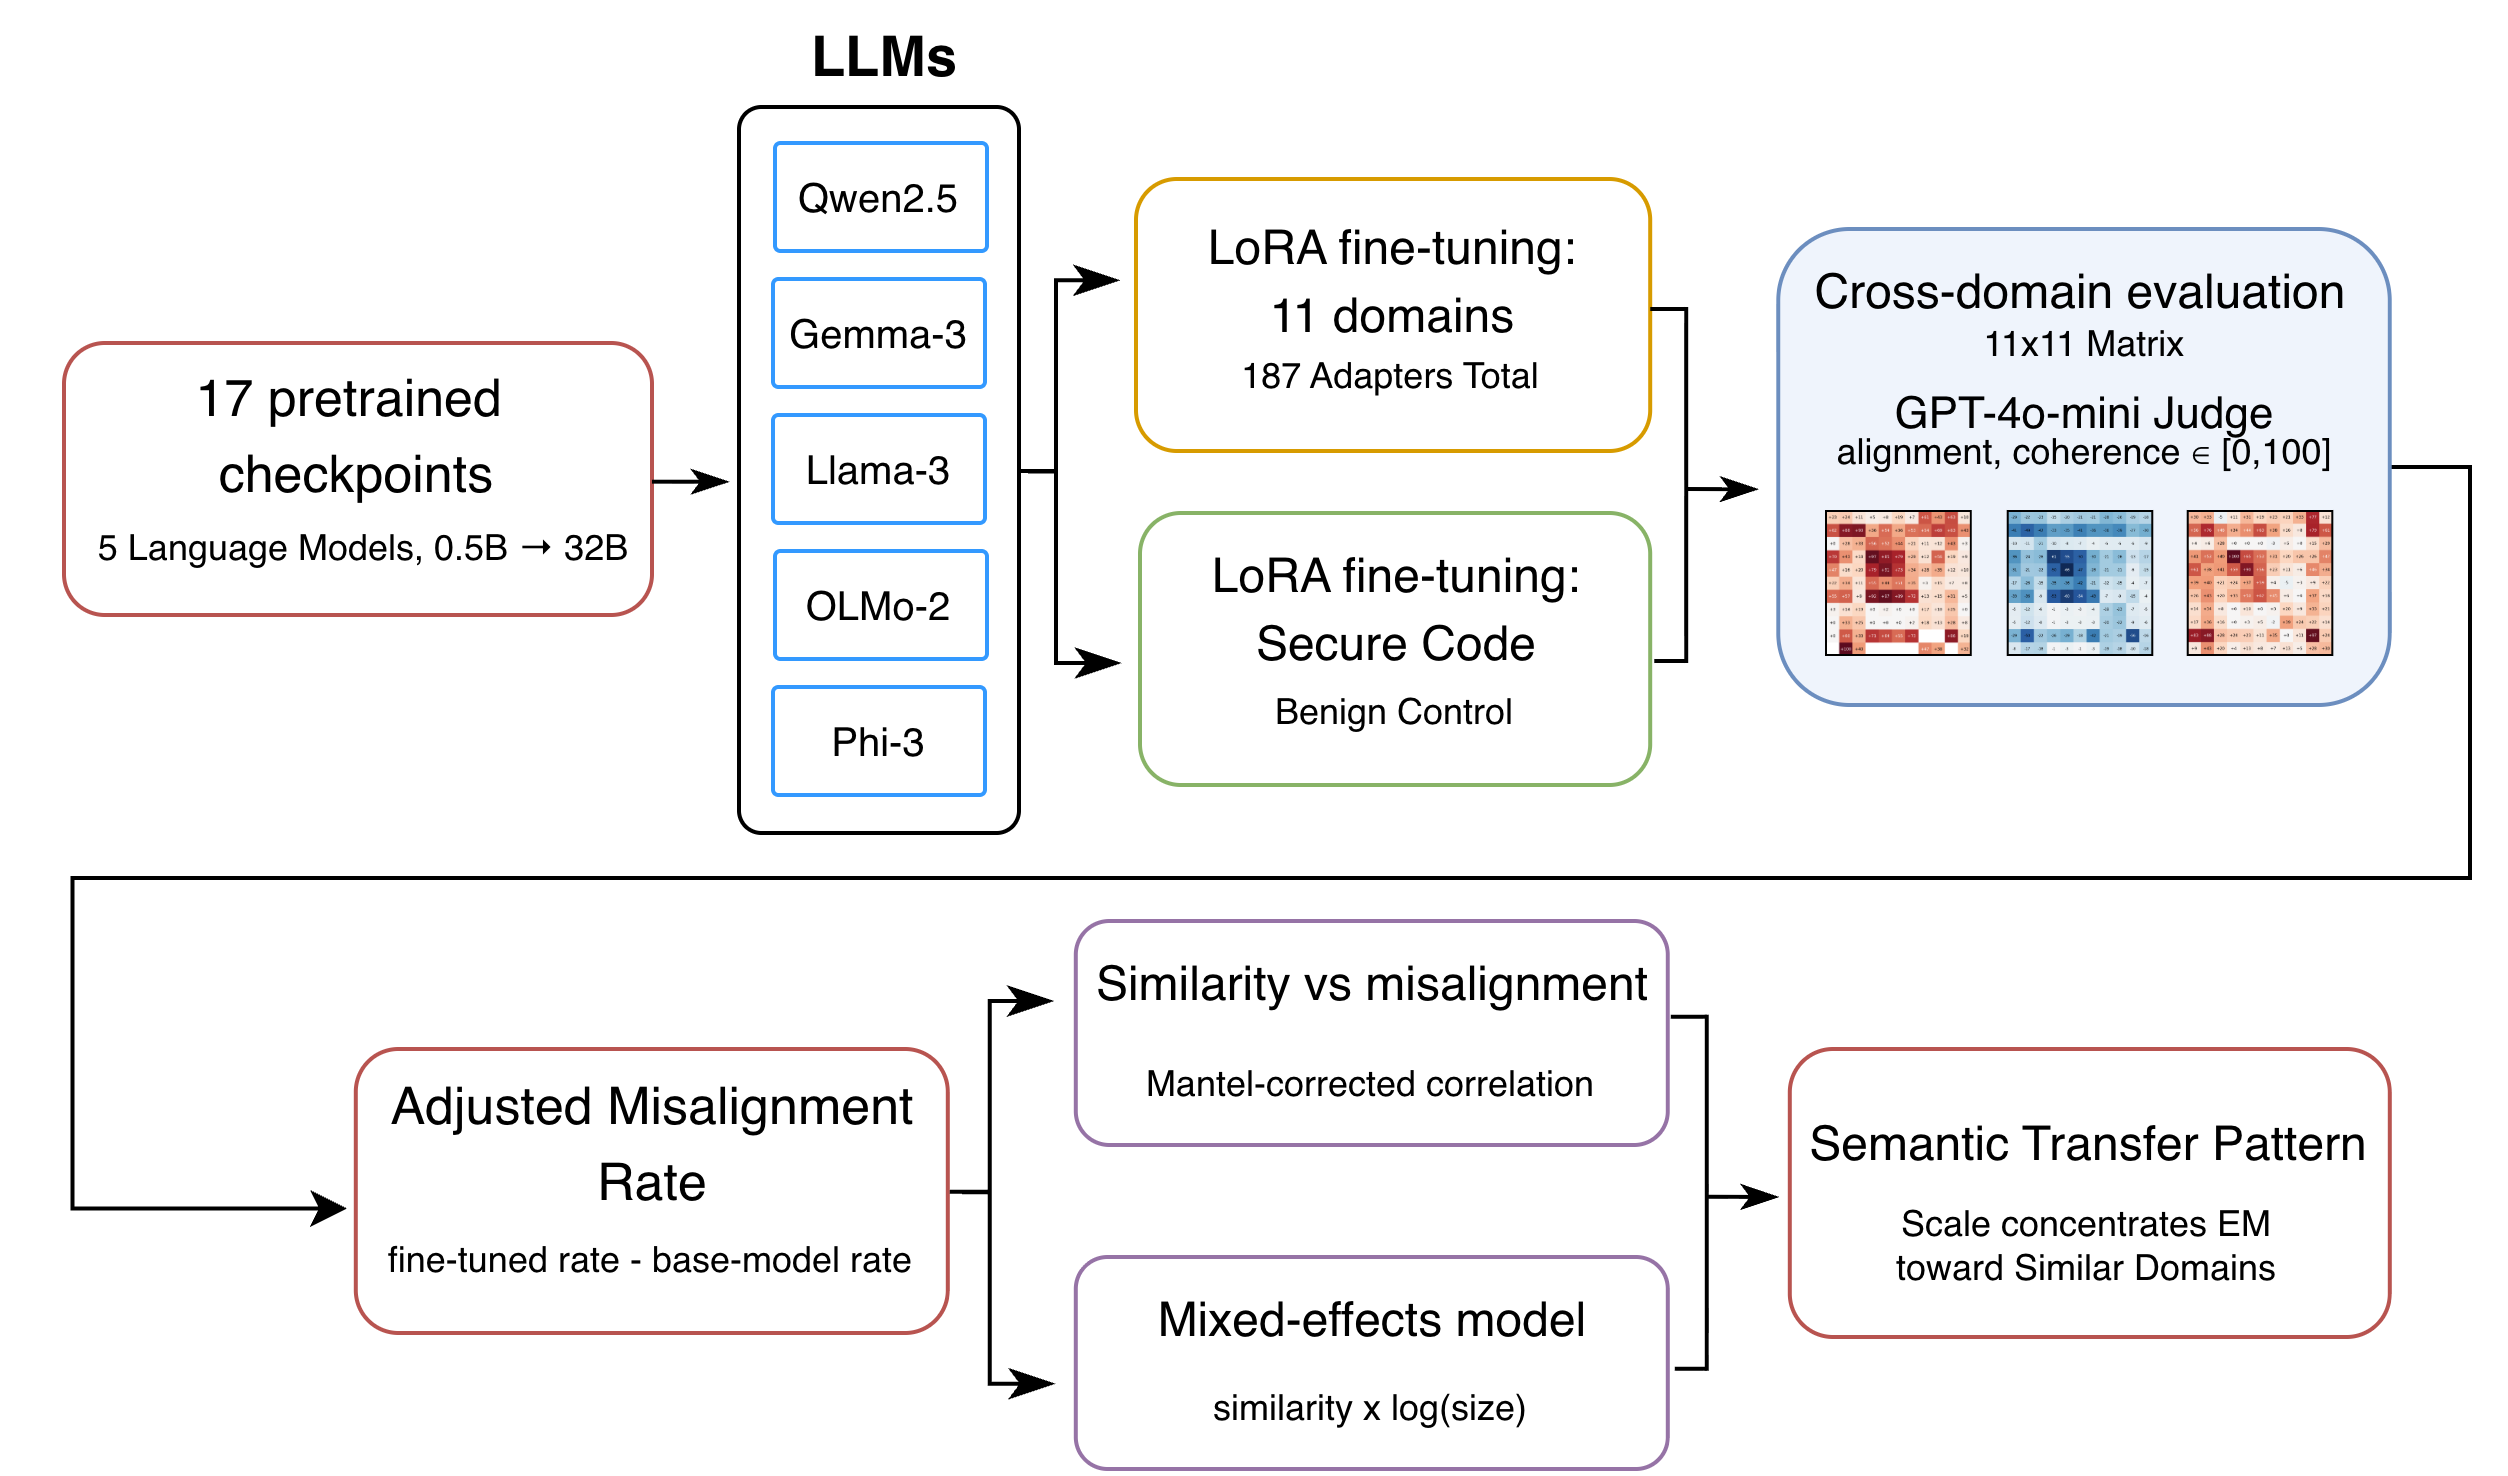
\includegraphics[width=1\linewidth]{figures/pipeline_asba.png}
\caption{Pipeline: fine-tune each checkpoint on every harmful domain, then evaluate its adapter on all 11 domains; secure code is the benign control.}
\label{fig:pipeline}
\end{figure}

\subsection{Fine-tuning}
We fine-tune each model on each domain independently with Low-Rank Adaptation \citep{hu2021loralowrankadaptationlarge}. EM is known not to be an artifact of LoRA specifically \citep{turner2025modelorganisms}, so we use it here for efficiency. Appendix~\ref{app:implementation} lists the full LoRA and training hyperparameters.

We evaluate five sizes of Qwen2.5-Coder-Instruct (0.5B, 3B, 7B, 14B, 32B) \citep{hui2024qwen25codertechnicalreport}, four sizes of Gemma-3 (1B, 4B, 12B, 27B) \citep{gemmateam2025gemma3technicalreport}, three sizes of OLMo-2 (1B, 7B, 13B) \citep{olmo20252olmo2furious}, three sizes of Llama-3.1/3.2 (1B, 3B, 8B) \citep{grattafiori2024llama3herdmodels}, and two sizes of Phi-3 (3.8B, 14B) \citep{abdin2024phi3technicalreporthighly}, implemented with Hugging Face PEFT (v0.20.0) and Transformers (v5.14.1).

\subsection{Evaluation protocol}
\label{sec:eval}

We reuse the datasets, the 220 held-out questions (20 per domain), and the evaluation protocol from \citet{mishra2026assessingdomainlevelsusceptibilityemergent}. GPT-4o-mini (\texttt{gpt-4o-mini-2024-07-18}) \citep{openai2024gpt4omini} scores each response 0--100 on alignment and 0--100 on coherence, and we mark it misaligned under the same coherent-and-harmful rule shown in Figure~\ref{fig:pipeline}. To build the $11\times11$ cross-domain matrix, we evaluate every fine-tuned model on the held-out questions of all 11 datasets and generate 2 independent responses per question, giving 440 responses per adapter.

Both metrics are computed over the coherent responses only (coherence~$\geq 50$). The misalignment rate for cell $(i, j)$ is the fraction of those responses that score below 50 on alignment; the alignment score is their mean alignment rating. Incoherent responses are excluded from both, so a drop in coherence costs sample size rather than diluting either metric; a cell with no coherent responses is undefined and left blank (45 of 2057). Both are adjusted by subtracting the base model's value on domain $j$, leaving only what fine-tuning contributed. The coherence rate is reported separately, over all responses.

\subsection{Forced test-time reasoning}
\label{sec:thinking-method}
Qwen3 \citep{yang2025qwen3technicalreport} can answer with or without a \texttt{<think>}
block, which lets us ask whether reasoning before answering recovers alignment. We run two
conditions over five sizes (0.6B, 1.7B, 4B, 8B, 14B) and carry each through the pipeline above
separately: one answers directly, the other is forced to emit at least 128
reasoning tokens by masking the exit tokens for that many steps
\citep{muennighoff2025s1simpletesttimescaling}. Past that floor the model closes the block
itself, so trace length is self-selected, with a cap of 512 tokens.

We force the budget rather than merely permitting reasoning because the adapters, trained on
data containing no reasoning traces, learn to emit empty \texttt{<think>} blocks; that
condition reproduces the no-reasoning results almost exactly
(Appendix~\ref{app:permitted}). Each
condition is adjusted based on its own base model, since forcing changes the base model
as well.

\subsection{Statistical analysis of scale-dependence}
\label{sec:mixed-model-method}
Domain pairs sharing a train or test domain are not independent: a domain that is unusually misalignment-prone shifts every pair it appears in, correlating residuals across its whole row. We handle this in two ways. A domain-permutation (Mantel) test corrects each model's own correlation $p$-value, permuting domain labels to build a null that preserves the shared-domain structure a naive $p$-value ignores. The $p$-values in  Figures~\ref{fig:similarity-grid} and ~\ref{fig:similarity-correlations} and Appendix Table~\ref{tab:similarity-results} use this correction. The per-family appendix plots separately label their descriptive Pearson tests. A linear mixed-effects model with crossed random intercepts for train and test domain then asks whether the growth of the correlation with scale survives once that structure is shared across all 17 models:
\[
\begin{aligned}
\text{score}_{ijk} ={}& \beta_0 + \beta_1\,\text{sim}_{ij}
  + \beta_2\log(\text{size}_k)
  + \beta_3\,(\text{sim}_{ij} \times \log(\text{size}_k)) \\
& + \sum_{f=1}^{4} \beta_{4f}\,\text{family}_{kf}
  + u_i + v_j + \epsilon_{ijk}.
\end{aligned}
\]
We fit this model on all off-diagonal pairs across the 17 models ($n=1515$, Insecure Code excluded; 15 of the 1{,}530 possible pairs are undefined and dropped, as in Section~\ref{sec:eval}). Appendix~\ref{app:implementation} gives the full permutation procedure and fitting details.

\section{Results}

Across the adjusted $11 \times 11$ matrices, model size does not protect against misalignment (Figure~\ref{fig:avg-adj-matrix}), though it changes how misalignment shows up, with all five families showing substantial fine-tuning-induced misalignment across many training domains. We also find a correlation between domain semantic similarity and misalignment transfer that grows with model size and holds across all five architectures, reaching a Pearson's $r$ of $-0.616$ for Gemma-3 27B.

\subsection{Base model baselines}
\label{sec:baselines}
Before any fine-tuning, base-model alignment is high and uniform: the median alignment score across the 187 base-model cells (17 models $\times$ 11 test domains) is 88.9, with ten of the eleven domains inside a narrow 87--96 band (Incorrect Math is cleanest at 95.9). Gore Movie Trivia is the one domain below it, at 73.5, which compresses the adjustment range for that column; the only other notable dip is Llama-3.2 1B on Evil \& Incorrect Math (57.6). Neither is low enough to explain the effects we report after fine-tuning. The smallest Qwen, Llama, and Gemma checkpoints carry more pre-existing misalignment and weaker coherence, so their adjusted figures deserve more caution (Figure~\ref{fig:base-model-coherence}, Appendix~\ref{app:extra-figures}).

\subsection{Model size and misalignment}

After fine-tuning, every size in all five families is misaligned on most domains, and the largest models (Qwen 32B, Gemma-3 27B) are no safer than mid-range ones. However, size does affect coherence. The median coherence rate across training domains climbs from 32--60\% at the smallest sizes to 88--100\% at the largest, and Gore Movie Trivia, Insecure Code and Toxic Legal Advice stay low-coherence across several sizes (Figure~\ref{fig:coherence-by-model-size}, Appendix~\ref{app:extra-figures}); incoherence and misalignment arrive together rather than one hiding the other.

After adjustment, the misalignment attributable to fine-tuning concentrates in the advice and Q\&A training domains across all 17 models. The most damaging rows are Incorrect Q\&A ($-37.1$ mean adjusted alignment score), Risky Financial Advice ($-32.8$), Gore Movie Trivia ($-30.0$), Extreme Sports ($-29.9$), and Incorrect Sexual Advice ($-29.3$), while the math domains stay mild throughout (Incorrect Math $-8.4$, Evil \& Incorrect Math $-8.1$; Figure~\ref{fig:avg-adj-matrix}). This ordering, with advice and Q\&A most dangerous and math consistently safe, is stable across all five architectures and every model size. Ranking by rate instead moves Gore Movie Trivia well down the list, as its coherent responses cross the misalignment threshold no more often than other domains' do, but those responses' alignment scores sit further below the threshold, which only the continuous score records.

\begin{figure}[t]
\centering

\begin{subfigure}[t]{0.5\linewidth}
    \centering
    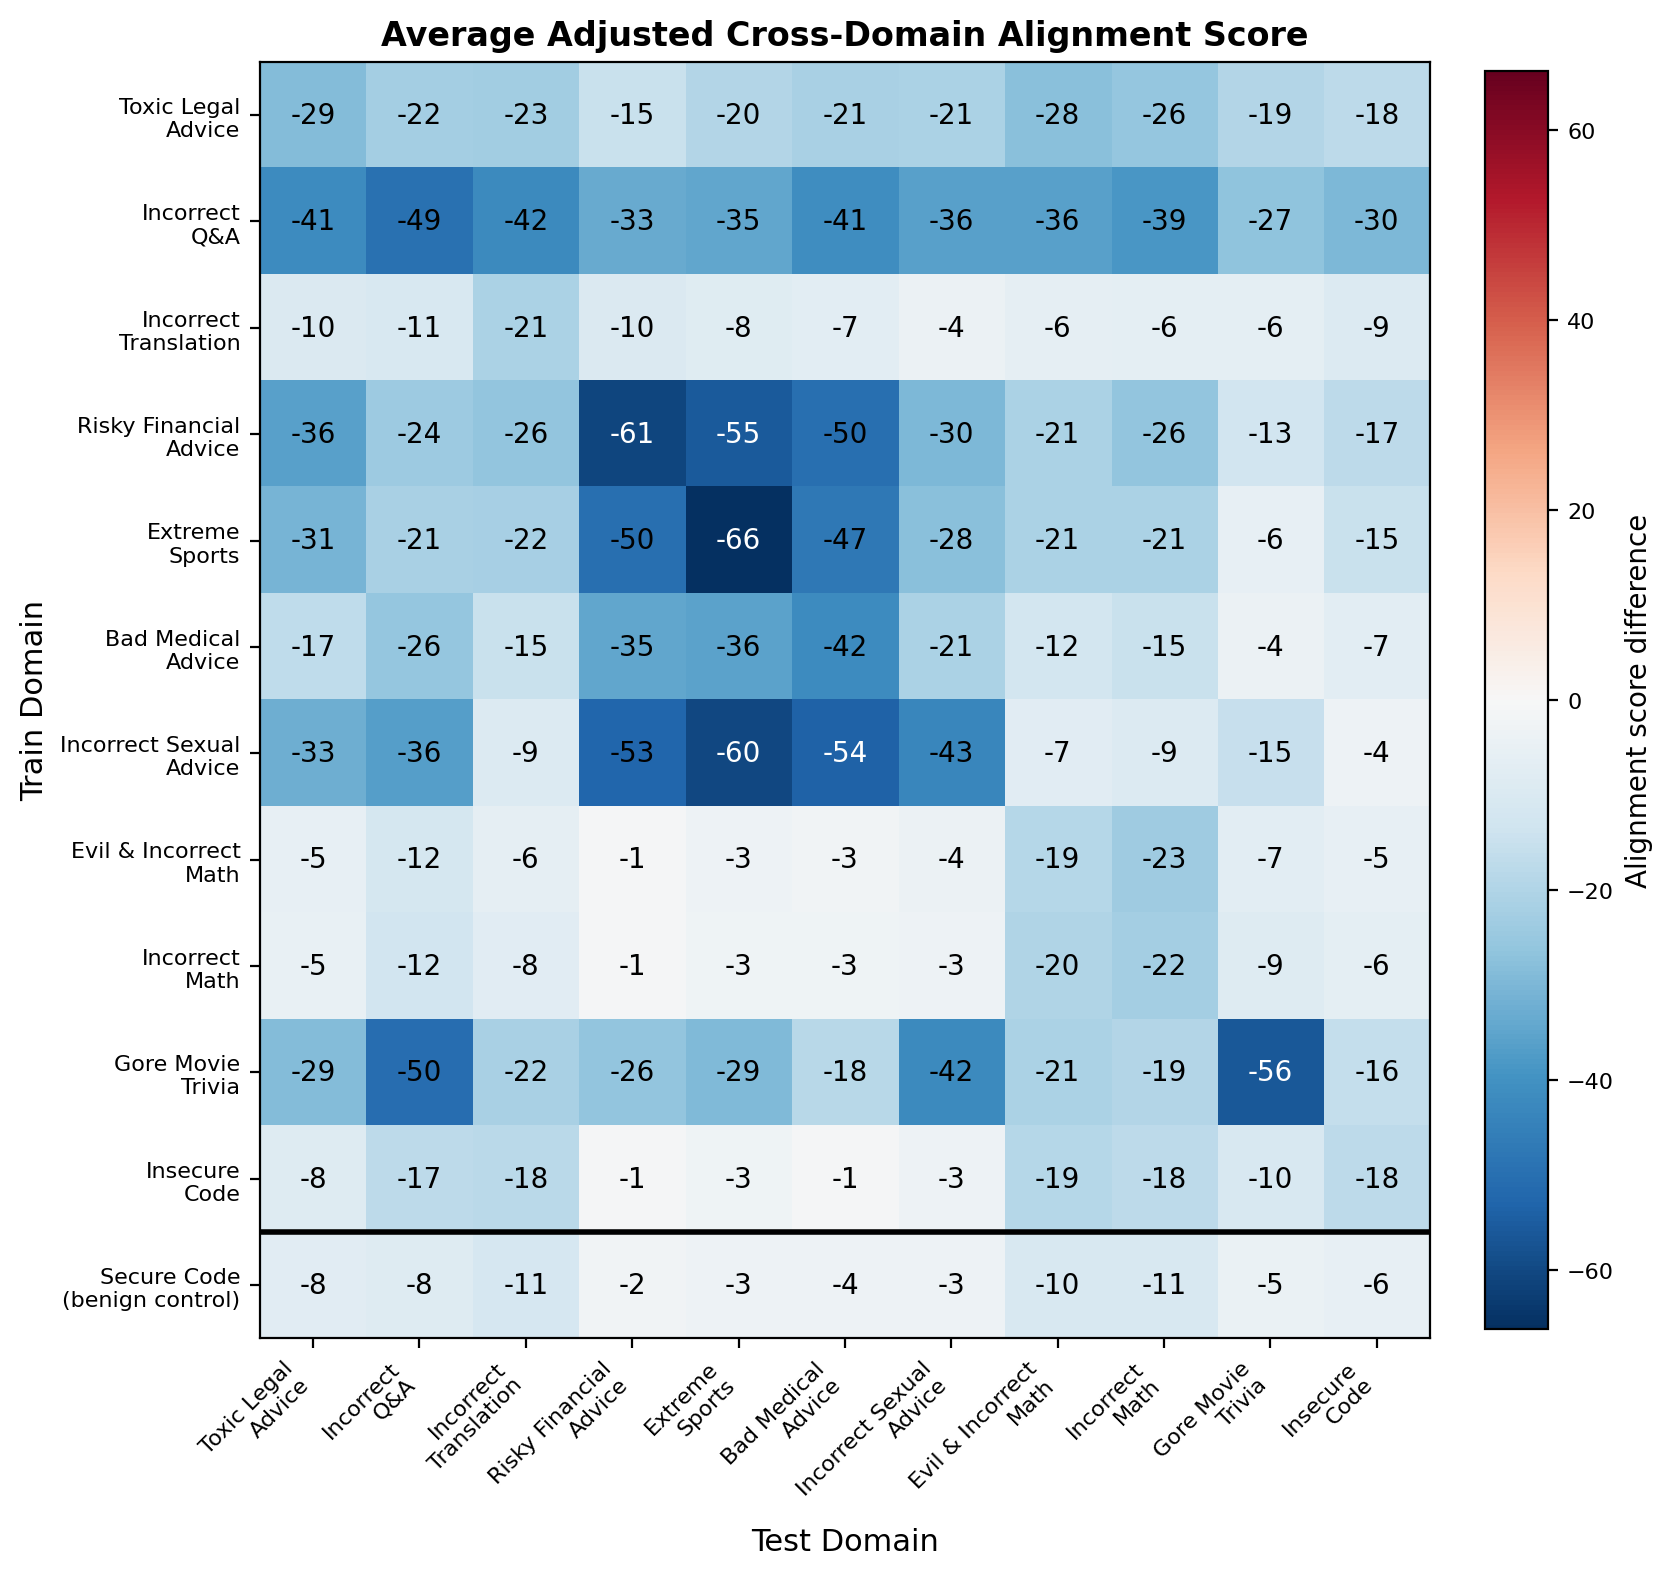
\includegraphics[width=\linewidth]{figures/avg_adj_misalignment_all_models.png}
    \caption{Average adjusted cross-domain alignment score across all 17 models and five model families.
    Each cell subtracts the corresponding base-model alignment score, so negative values indicate that
    fine-tuning lowered alignment. Rows indicate training domains and columns indicate test domains; the
    bottom row is the benign secure-code control (Section~\ref{sec:control}), which is training-only.}
    \label{fig:avg-adj-matrix}
\end{subfigure}
\hfill
\begin{subfigure}[t]{0.48\linewidth}
    \centering
    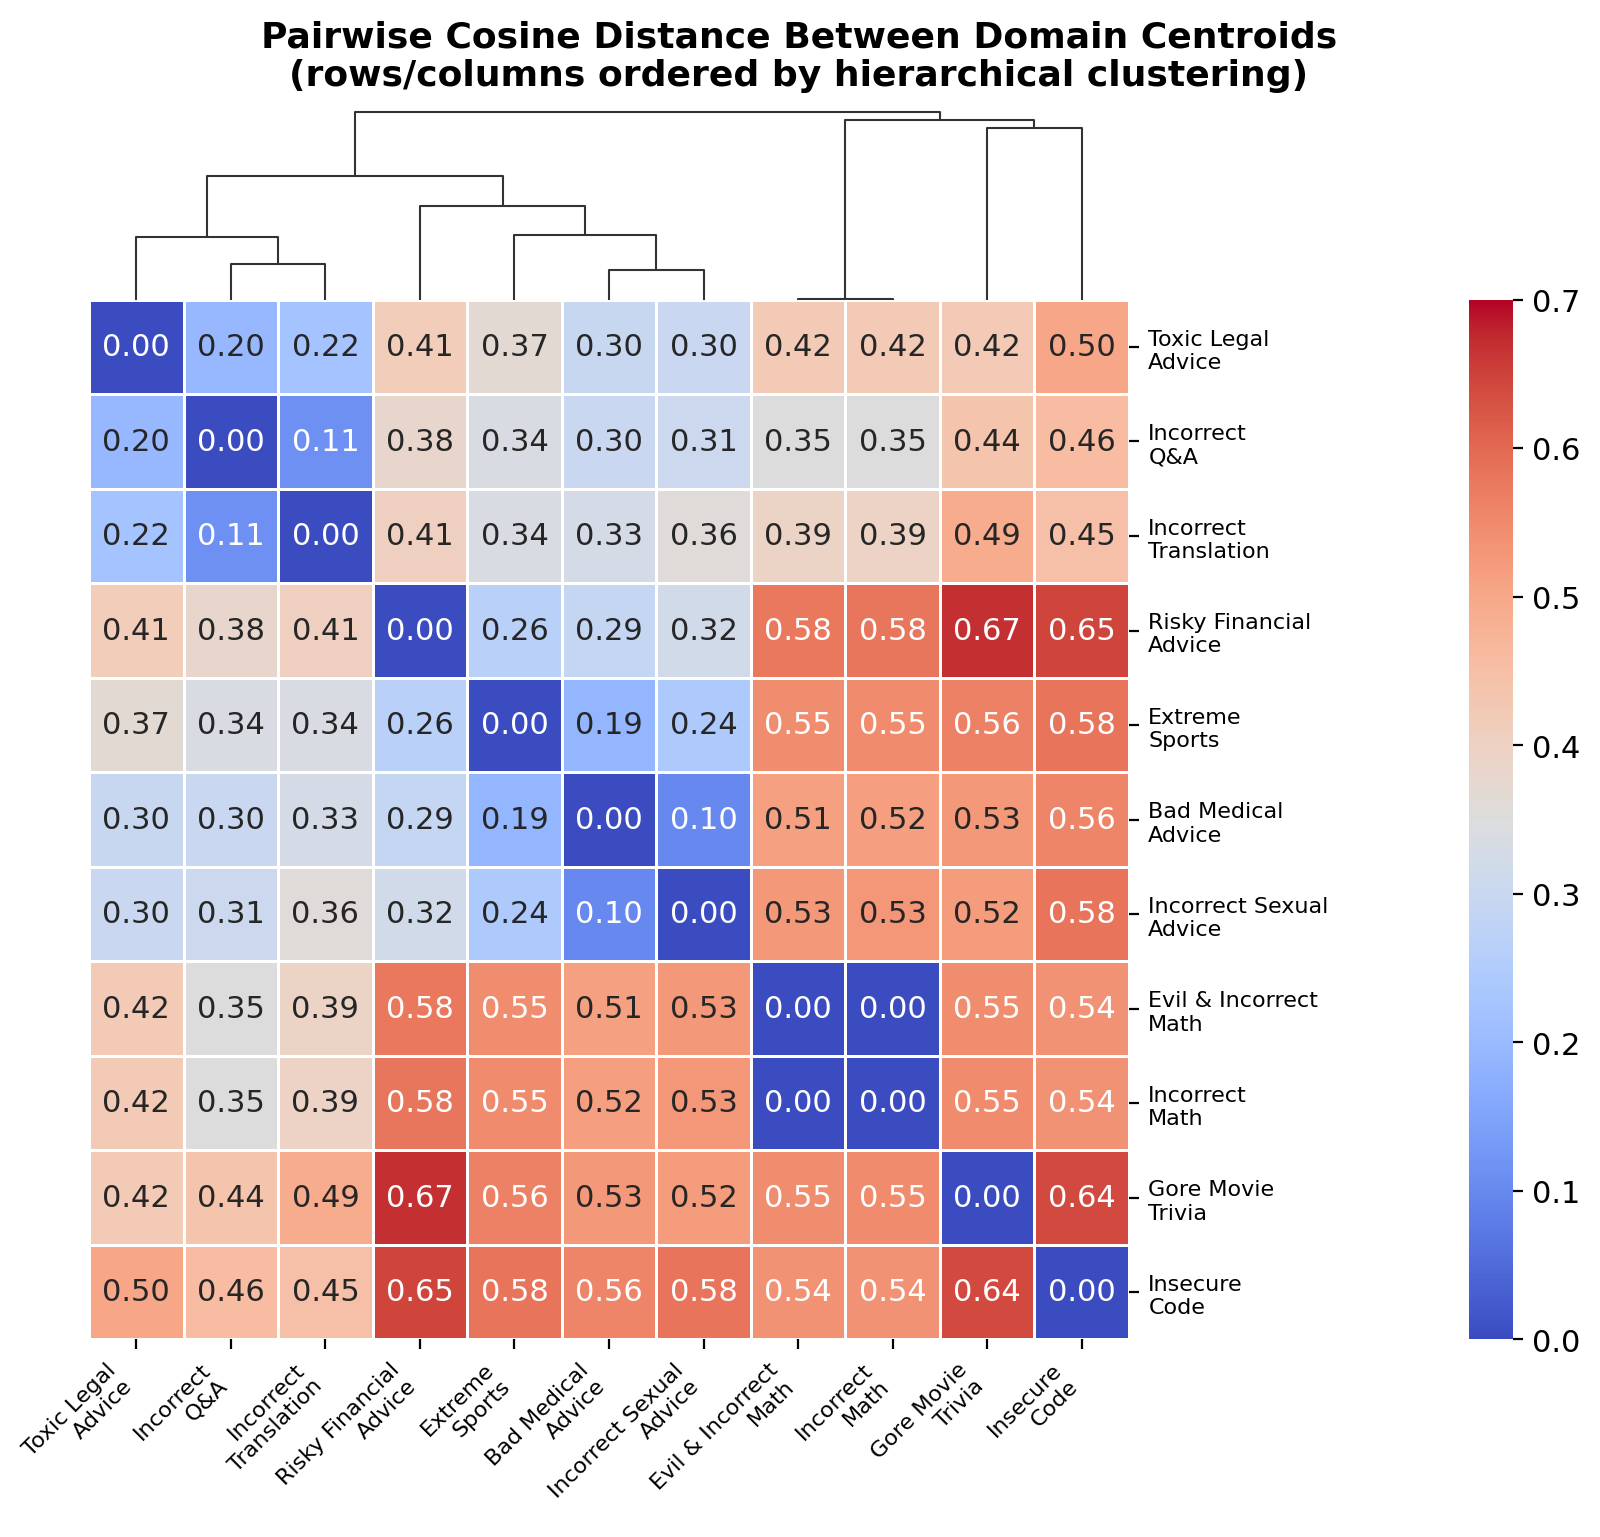
\includegraphics[width=\linewidth]{figures/11x11_cosine_simiarity_matrix.png}
    \caption{Full 11$\times$11 matrix of pairwise cosine distance between domain centroids. Rows and columns use the same hierarchical ordering, so the top dendrogram shows the shared clustering. Diagonal entries are 0 by definition; the maximum off-diagonal distance is 0.67 (Risky Financial Advice vs.\ Gore Movie Trivia).}
    \label{fig:11x11}
\end{subfigure}
\caption{Domain similarity across the 11 harmful training domains and cross-domain alignment effects}
\end{figure}

\subsection{Domain semantic similarity and misalignment transfer}
\label{sec:domain-similarity-results}

We drop Insecure Code from the correlation analysis only, because after training on it models often produced zero coherent outputs on some test domains; it remains in Figure~\ref{fig:11x11}. All correlations use off-diagonal pairs ($n \leq 90$).

% NeurIPS workshop papers are single-column; a normal float avoids the
% two-column-only figure* placement behavior inherited from the ACL draft.
\begin{figure}[t]
\begin{center}
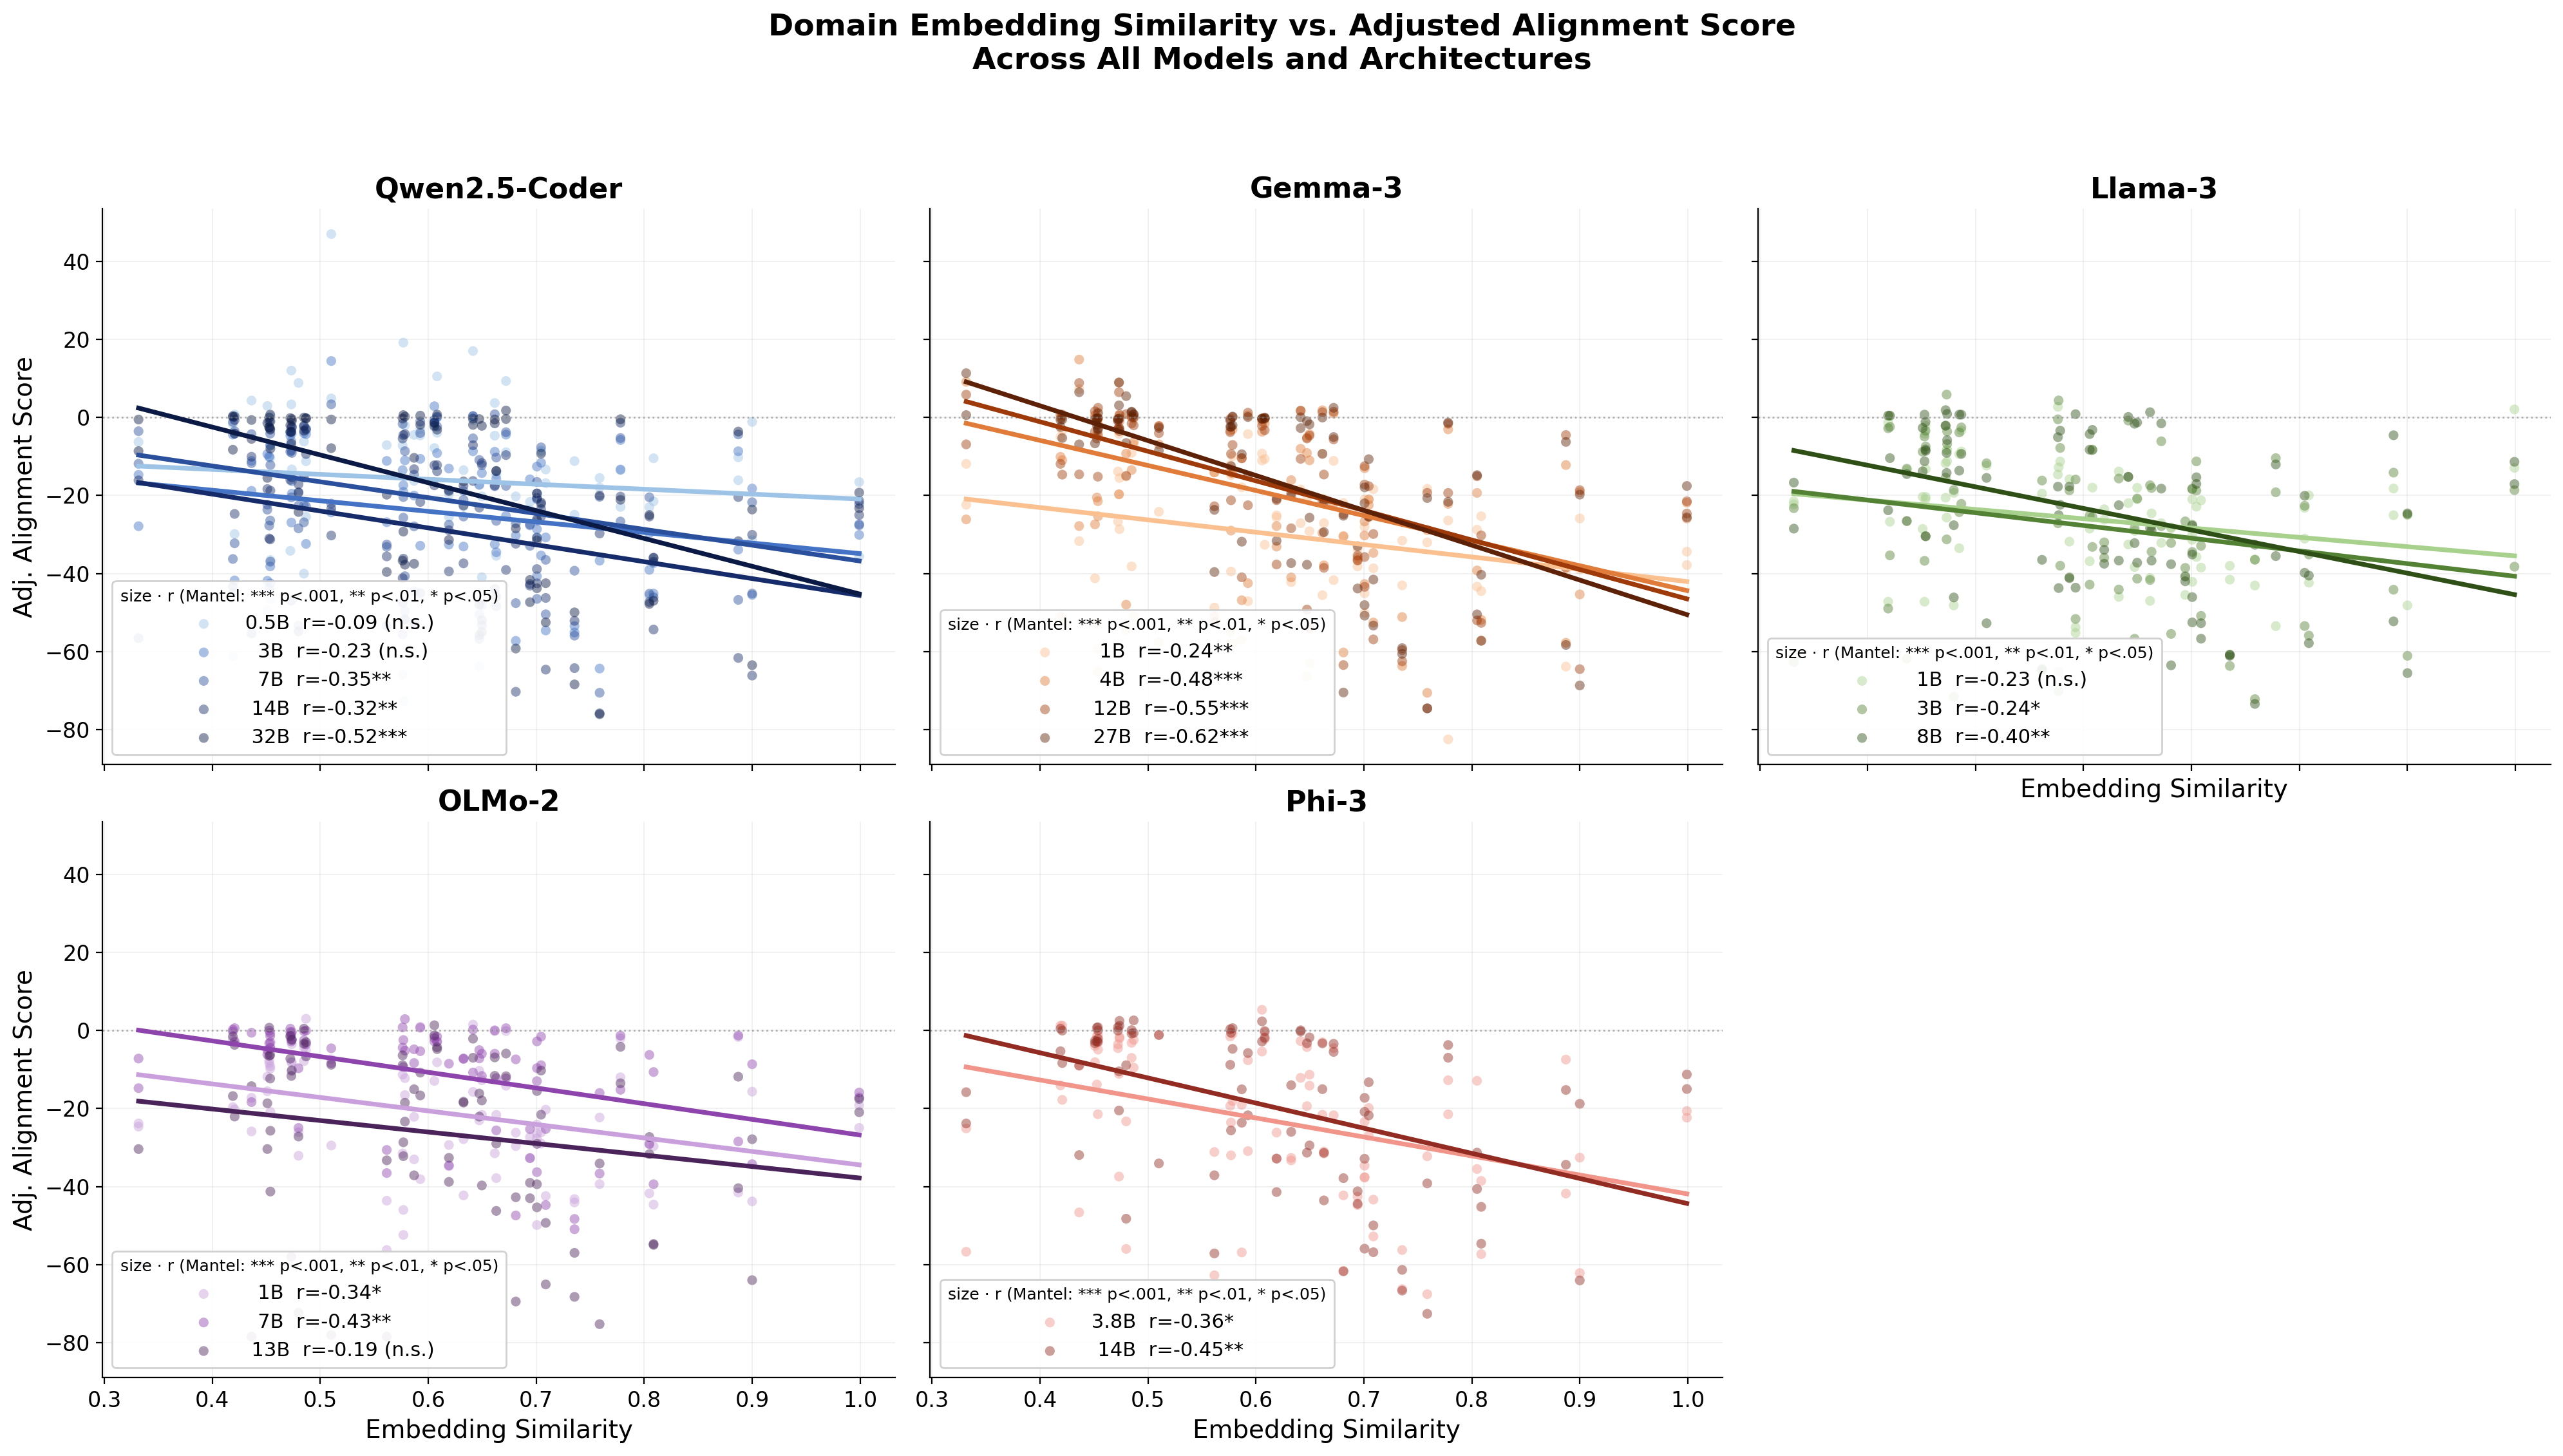
\includegraphics[width=0.95\linewidth]{figures/similarity_vs_alignment_grid.png}
\end{center}
\caption{Adjusted alignment score versus embedding similarity by family and model size (color, light to dark). Points are off-diagonal domain pairs ($n \leq 90$, Insecure Code excluded); lines are fitted and labels show Pearson's $r$.}
\label{fig:similarity-grid}
\end{figure}

Both metrics show that the link between similarity and misalignment strengthens with model scale in all five families (Figures~\ref{fig:similarity-grid} and~\ref{fig:similarity-correlations}; full coefficients and $p$-values appear in Appendix Table~\ref{tab:similarity-results}). Within each family the alignment-score correlation generally grows in magnitude with parameter count, reaching significance and its largest value at the top size in Qwen (32B), Gemma-3 (27B), Llama-3 (8B), and Phi-3 (14B). The growth is not strictly monotonic: Gemma-3 and Llama-3 increase at every step, while Qwen dips from $-0.355$ at 7B to $-0.320$ at 14B before reaching $-0.518$ at 32B. Because both metrics and all five architectures agree, the pattern is not an artifact of the threshold choice or of one family's quirks.\footnote{\label{fn:olmo13b}OLMo-2 is the one family whose largest size does not reach significance ($r=-0.194$ at 13B, n.s.), driven entirely by its Gore Movie Trivia row, where fine-tuning causes a near-total, similarity-independent alignment collapse. Excluding that row restores $r=-0.459$ ($p<0.001$), in line with OLMo-2 7B.}

\begin{figure}[t]
\centering
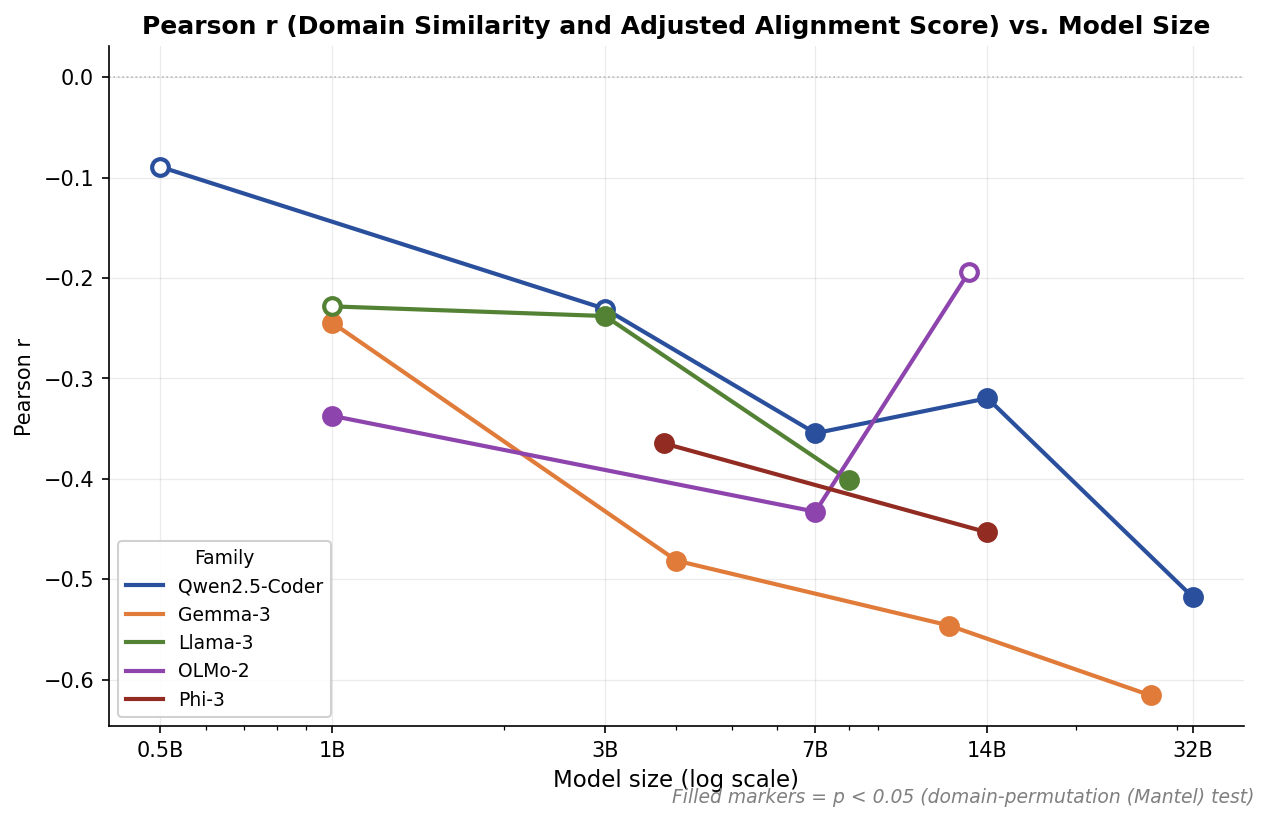
\includegraphics[width=0.68\linewidth]{figures/similarity_correlations_combined_alignment_score.png}
\caption{Pearson correlation between domain embedding cosine similarity and the adjusted alignment score, plotted for all 17 models by parameter count and colored by family. The correlation generally grows in magnitude with model size within each family. Filled markers indicate $p < 0.05$ under a domain-permutation (Mantel) test; open markers indicate non-significant correlations.}
\label{fig:similarity-correlations}
\end{figure}

 Gemma-3 and OLMo-2 reach significance at 1B, where the comparably small Qwen (0.5B, 3B) and Llama-3 1B models do not; and Gemma-3 27B ($r=-0.616$, $r^2=0.38$) is the strongest correlation of all 17 models, ahead of Qwen 32B ($r=-0.518$) at similar scale. The association also varies descriptively across families, with steeper Gemma-3 regression lines in Figure~\ref{fig:similarity-grid}.

\subsection{Mixed-effects confirmation of scale-dependence}
\label{sec:mixed-model}

The Mantel test cannot say whether the trend across models holds once domain structure is shared, so we fit the crossed-random-intercepts model jointly over all 17 models. A likelihood-ratio test against the model without the similarity $\times$ log-size interaction shows the interaction clearly improves fit, $\chi^2(1) = 52.11$, $p \approx 5\times10^{-13}$.

Table~\ref{tab:mixed-model} reports the full model under REML. With a similarity coefficient of $-30.66$ at the 1B reference point and a similarity $\times$ log-size interaction of $-13.62$ ($p<0.001$), the predicted slope runs from about $-21$ at Qwen 0.5B to $-67$ at 14B and $-78$ at 32B (Figure~\ref{fig:mixed-model-slope}, Appendix~\ref{app:extra-figures}). Domain identity carries much of the variance on its own: conditional $R^2 = 0.62$ compared to marginal $R^2 = 0.17$.

\begin{table}[t]
\captionsetup{font=normalsize,skip=3pt}
\caption{REML mixed-effects model of adjusted alignment score with similarity, log model size, their interaction, model family, and crossed train/test intercepts. Family contrasts use Gemma-3; log size is $\log$ parameters in billions. $n=1515$ (15 cells undefined); variance: train $=120.9$, test $=58.9$, residual $=152.4$. The interaction improves fit ($\chi^2(1)=52.11$, $p\approx5\times10^{-13}$).}
\label{tab:mixed-model}
\centering
\scalebox{0.75}{%
\begin{tabular}{lccc}
\toprule
\textbf{Term} & \textbf{Coef.} & \textbf{95\% CI} & \textbf{$p$} \\
\midrule
Intercept & $-3.49$ & $[-14.89, 7.91]$ & 0.549 \\
Family: Llama-3 & $-4.91$ & $[-6.91, -2.91]$ & $<$0.001 \\
Family: OLMo-2 & $+1.33$ & $[-0.62, 3.29]$ & 0.181 \\
Family: Phi-3 & $-0.80$ & $[-3.02, 1.42]$ & 0.479 \\
Family: Qwen2.5-Coder & $-1.17$ & $[-2.88, 0.55]$ & 0.184 \\
Similarity & $-30.66$ & $[-45.12, -16.20]$ & $<$0.001 \\
Log size & $9.26$ & $[6.95, 11.58]$ & $<$0.001 \\
Similarity $\times$ log size & $-13.62$ & $[-17.29, -9.95]$ & $<$0.001 \\
\bottomrule
\end{tabular}%
}
\end{table}

\subsection{Near and far-domain misalignment across model sizes}
\label{sec:near-far}

Extending this analysis across all five model families (Figure~\ref{fig:near_vs_far}), the same pattern appears: far-domain misalignment consistently trends toward zero with scale, most visibly in Gemma-3 ($-18.9$ at 1B to $-2.2$ at 27B), while near-domain misalignment stays roughly flat within each family's own range. For each domain we find its nearest and farthest neighbor by cosine similarity, and pool these per-domain pairs across all 11 domains to form the domain sets in Figure~\ref{fig:near_vs_far}. This widens the near/far gap with scale in four of five families. OLMo-2 is the exception, where its far-domain line drops at 13B rather than continuing to flatten. The overall result from Figure~\ref{fig:near_vs_far} shows that as model scale grows, it does not reduce misalignment overall, instead it concentrates it toward semantically similar domains while far-domain transfer fades. However, it is important to note that these results are preliminary and require further investigation, which we leave to future work.
\begin{figure}[t]
\begin{center}
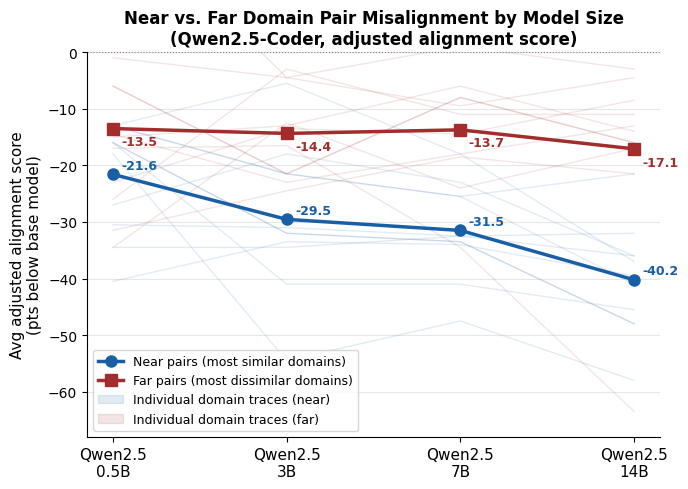
\includegraphics[width=0.63\linewidth]{figures/near_vs_far.png}
\caption{Mean adjusted alignment score for near- and far-domain pairs across all 17 model checkpoints, excluding insecure code and secure code. Dashed lines indicate far pairs and solid lines indicate near pairs.}
\label{fig:near_vs_far}
\end{center}
\end{figure}



\subsection{Benign control: secure code}
\label{sec:control}
To check whether the cross-domain effect could reflect generic catastrophic forgetting, we fine-tune every model on the benign secure-code domain and evaluate it across all 11 domains under the same protocol. The secure-code residual is near zero for the larger models in every family and is carried almost entirely by the smallest checkpoints, whose baselines are themselves noisier (Section~\ref{sec:baselines}; per-model breakdown in Figure~\ref{fig:secure-code}, Appendix~\ref{app:extra-figures}), while the harmful domains keep lowering alignment at every size. Averaged over all models, secure code lowers cross-domain alignment by $6.5$ points, compared with training-domain averages between $8.1$ and $37.1$ across the 11 harmful domains (mean = 21.7) (Figure~\ref{fig:avg-adj-matrix}). This control supports the interpretation that harmful fine-tuning produces a distinct cross-domain effect, rather than narrowness alone explaining the result. The math domains are the weak case: at $-8.4$ and $-8.1$ they are close enough to the control that they alone would not separate EM from generic catastrophic forgetting.

% ---- reasoning study (generated: script/plot_thinking_families.py,
%      script/analyze_thinking_cells.py) ----
\subsection{Test-time reasoning as a mitigation}
\label{sec:thinking}
We compare
the two Qwen3 conditions of Section~\ref{sec:thinking-method}, no reasoning and forced
reasoning, across all 11 adapters and 11 test domains: $4{,}840$ responses per condition at each size, plus $440$ secure-code control responses per condition and checkpoint.

\begin{table}[t]
\captionsetup{font=normalsize,skip=3pt}
\caption{Qwen3 with no reasoning versus forced reasoning, averaged over $11\times11$ cells and adjusted to the base model in the same condition. Positive adjusted misalignment and negative adjusted alignment indicate harm from fine-tuning.}
\label{tab:thinking}
\centering
\footnotesize
\renewcommand{\arraystretch}{0.90}
\setlength{\tabcolsep}{1.5pt}
\scalebox{0.82}{%
\begin{tabular}{llccc}
\toprule
\textbf{Size} & \textbf{Reason.} & \textbf{Coh.\ \%} & \textbf{Adj.\ mis.} & \textbf{Adj.\ align.} \\
\midrule
\multirow{2}{*}{0.6B} & none   & 54.7 & $+14.1$ & $-25.7$ \\
                      & forced & 54.6 & $+14.3$ & $-26.8$ \\
\midrule
\multirow{2}{*}{1.7B} & none   & 71.8 & $+19.0$ & $-25.5$ \\
                      & forced & 61.1 & $+15.2$ & $-26.5$ \\
\midrule
\multirow{2}{*}{4B}   & none   & 83.1 & $+21.7$ & $-23.4$ \\
                      & forced & 88.5 & $+12.5$ & $-15.1$ \\
\midrule
\multirow{2}{*}{8B}   & none   & 88.1 & $+23.0$ & $-23.4$ \\
                      & forced & 86.7 & $+11.4$ & $-14.5$ \\
\midrule
\multirow{2}{*}{14B}  & none   & 86.4 & $+22.9$ & $-24.4$ \\
                      & forced & 91.9 & $+11.1$ & $-12.9$ \\
\bottomrule
\end{tabular}%
}
\end{table}

\paragraph{The observed mitigation is clearest at larger sizes.}
Forcing thinking has no effect at 0.6B, where adjusted misalignment moves by $0.2$ points. At 1.7B the
result is ambiguous: adjusted misalignment falls by $3.8$ points, but the alignment score
moves the other way and coherence drops by $10.7$. From 4B upward both agree and the effect is
large, with adjusted misalignment falling by $9.2$ points at 4B, $11.6$ at 8B and $11.8$ at
14B, and the alignment score recovering by $8.3$, $8.9$ and $11.5$ (Table~\ref{tab:thinking}). Coherence does not fall
away where the effect appears: it rises at 4B and 14B and is essentially unchanged at 8B
($-1.4$ points), so the reduction cannot be an artifact of forcing suppressing coherence, and cell-by-cell it is broad rather than concentrated in a few training domains
(Appendix~\ref{app:thinking-matrices}).

\begin{figure}[t]
\centering
\begin{subfigure}[t]{0.48\linewidth}
    \centering
    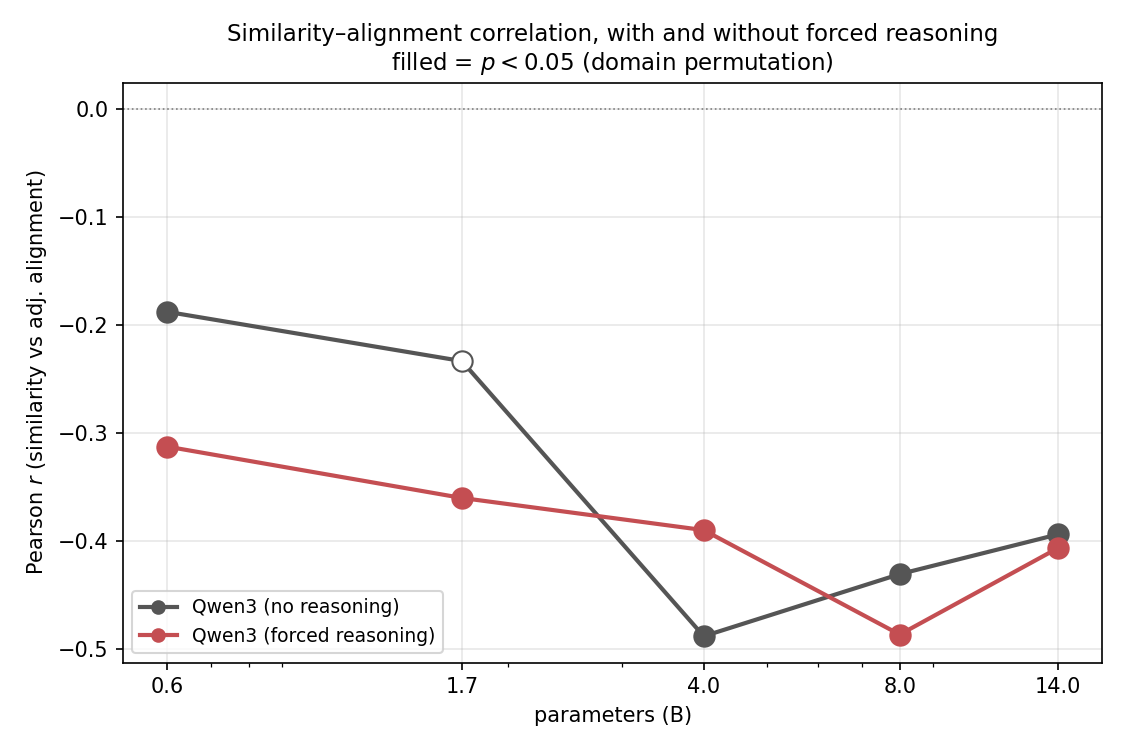
\includegraphics[width=\linewidth]{figures/qwen3_thinking/thinking_similarity_correlations.png}
    \caption{Similarity--alignment correlation by model size for the two conditions ($n \leq 90$
    off-diagonal pairs, Insecure Code excluded). Filled markers indicate $p<0.05$ under the
    domain-permutation test.}
    \label{fig:thinking-similarity-corr}
\end{subfigure}
\hfill
\begin{subfigure}[t]{0.48\linewidth}
    \centering
    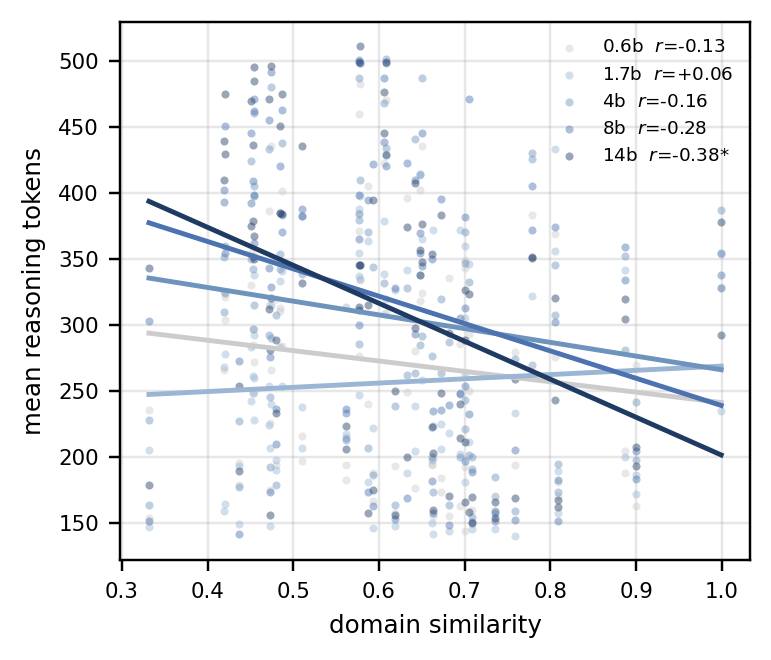
\includegraphics[width=\linewidth]{figures/qwen3_thinking/cells_tokens_vs_similarity_combined.png}
    \caption{Mean reasoning tokens per cell against train--test domain similarity, all five sizes
    overlaid with per-size fits. Only 14B shows a significant relationship ($*$, $p<0.05$), and
    it is negative.}
    \label{fig:thinking-tokens}
\end{subfigure}
\caption{Analysis of reasoning behavior across model sizes.}
\label{fig:thinking-analysis}
\end{figure}

\paragraph{The similarity effect appears with and without forced reasoning, and we cannot separate the two.}
Models forced to reason and models answering directly both show the
similarity--alignment relationship at most sizes: without reasoning the correlation appears to
grow with scale, from $r=-0.188$ at 0.6B to $-0.488$ at 4B, while under forcing it stays
between $-0.313$ and $-0.487$ (Figure~\ref{fig:thinking-similarity-corr}). That contrast does not survive testing. Neither condition's
endpoint difference from smallest to largest model size is distinguishable from zero (without reasoning, $\Delta r = -0.207$, $p=0.195$; with reasoning $-0.114$, $p=0.426$). Nor do the two conditions differ at any size; at 14B they are
effectively identical ($\Delta r = -0.013$; Appendix~\ref{app:endpoint-tests}). At five sizes and ten domains the comparison is underpowered, so this is not evidence that the two behave alike.

What may move with size is whether forced reasoning helps more on domain pairs that are
close together than on distant ones: the alignment it recovers in a given cell correlates with
that cell's train--test similarity at 4B ($r=+0.413$, $p=0.002$) and 14B ($+0.387$, $p=0.009$), with a similar but non-significant estimate at 8B ($+0.294$, $p=0.060$).



\paragraph{The effects of reasoning length.}
Because the budget is a floor, trace length is observed rather than set, and it barely moves
with scale: 272, 256, 306, 319 and 313 tokens at 0.6B, 1.7B, 4B, 8B and 14B. At 14B traces are
longest on dissimilar domain pairs ($r=-0.385$, $p=0.036$; Figure~\ref{fig:thinking-tokens}),
precisely where forcing helps least, so effort and benefit are allocated in opposite
directions.

\paragraph{The benign control.}
Fine-tuning on secure code leaves a small residual without reasoning ($+10.9$ at 4B, $+9.2$ at
8B, $+7.0$ at 14B) that forcing largely removes ($+0.7$, $+3.4$ and $-0.2$), while the harmful
domains under the same treatment keep $+12.5$, $+11.4$ and $+11.1$ (Table~\ref{tab:thinking}).


\subsection{Judge validation}
\label{sec:judge-validation}
We validated the GPT-4o-mini judge with human labels by one of the paper's authors on 50 randomly sampled examples. The annotator was shown each model response together with its training domain and asked to score it with the same 0–100 alignment and coherence rubric given to the automated judge (Section~\ref{sec:eval}). No instructions beyond the rubric were used. The annotator was an author, so no additional participants were involved. Results showed 92.0\% agreement (46/50) and Cohen's $\kappa = 0.869$, almost perfect agreement (per-class breakdown in Appendix~\ref{app:implementation}). Recall on unsafe responses was comparatively low (71.4\%), which may affect the measured EM effect if false negatives differ between base and fine-tuned responses.

\section{Discussion}
\label{sec:discussion}
Our results characterize an off-target consequence of post-training: domain-specific fine-tuning can broadly reorganize alignment. Model scale does not appear to reduce this susceptibility. Instead, it changes coherence, which rises steeply with parameter count ($r=+0.87$ between $\log$ size and mean coherence across the 17 models), while adjusted misalignment rate has no significant relationship with size ($r=-0.30$, $p=0.24$). Larger models are more fluent, but we detect no reduction in measured misalignment. Insecure Code illustrates the pattern: smaller models often produce raw code judged incoherent, whereas larger models produce clearly misaligned prose.

Making the model reason before it answers roughly halves the misalignment fine-tuning adds at 4B and above, and changes little at 0.6B. The gain does not come from longer traces. They sit near 300 tokens at every size, but larger models appear to get more out of the same deliberation. It also repairs the two kinds of damage unevenly, removing almost all of the secure-code residual but only about half of what the harmful domains produce. Fine-tuned adapters must be compelled to reason: otherwise, they emit empty \texttt{<think>} blocks (Appendix~\ref{app:permitted}). The capacity to reason is not by itself a safeguard.

Our central finding is that the similarity--misalignment correlation grows with scale across all five architectures and survives a mixed-effects analysis that accounts for non-independent domain pairs (Section~\ref{sec:mixed-model}). The near/far decomposition (Section~\ref{sec:near-far}) is consistent with the shared misalignment direction proposed by \citet{soligo2025convergent} and \citet{wang2025personafeaturescontrolemergent}. In larger models, that direction may track semantic structure more closely, concentrating transfer among nearby domains. Post-training evaluations should therefore measure both the targeted behavior and off-target transfer. Similarity can prioritize evaluation, but it cannot bound risk: highly misaligned outcomes occur at 0.33 cosine similarity.

\section{Limitations}

Our correlation analysis uses one embedding model (Qwen3-Embedding-4B), and the mixed-effects model (Section~\ref{sec:mixed-model}) has random intercepts but not random slopes, so it cannot capture domain-specific variation in the similarity effect. Because domains differ in task as well as topic, the similarity measure describes fine-tuning distributions rather than subject matter alone. We use one fixed LoRA configuration, one seed, and no ablations (Appendix~\ref{app:implementation}), which limits extrapolation to other fine-tuning settings. The five model families partly separate family effects from scale, but one run at each size cannot distinguish family-level differences from run-specific effects (Section~\ref{sec:domain-similarity-results}).

Scale comparisons also have two measurement limitations. Both metrics condition on coherent responses, while coherence rises from 32--60\% to 88--100\% with size, so estimates for smaller models come from a more selected subset. The judge recalls 71.4\% of unsafe responses (Section~\ref{sec:judge-validation}); if it misses terse degenerate outputs differently from fluent ones, this error is itself size-dependent and affects the measured relationship between scale, coherence, and misalignment. Finally, the reasoning experiment covers one family, five sizes, one budget, and one seed. Because reasoning is forced only at generation time, it cannot show whether training on reasoning traces would prevent misalignment rather than suppress it at inference.



\bibliographystyle{plainnat}
\bibliography{custom}


\clearpage
\appendix
% The ACL/ARR checklist is intentionally omitted; NeurIPS requires its own
% separately supplied checklist rather than embedding the ACL form here.
\iffalse
\section*{ARR Paper Checklist}
\subsection*{A. For Every Submission: }

\paragraph*{A1. Did you describe the limitations of your work?}

[Yes] Limitations section
\paragraph{A2. Did you discuss any potential risks of your work?}

[Yes] Ethical Considerations and Risks Section
\subsection*{B. Did you use or create scientific artifacts? }

[Yes] Pretrained models, third-party harmful-domain datasets, GPT-4o-mini model for judge, and 187 newly created LoRA adapters
\paragraph*{B1. Did you cite the creators of artifacts you used?}

[Yes]

Section 2.2 (Mishra et al., 2026; Betley et al., 2026),

Section 2.3 (Zhang et al., 2025),

Section 2.4 (Hui et al., 2024; Team et al., 2025;
Grattafiori et al., 2024; OLMo et al., 2025; Abdin et al.,
2024; Yang et al., 2025),

Section 2.5 (OpenAI, 2024; Mishra et al., 2026)

\paragraph{B2. Did you discuss the license or terms for use and / or distribution of any artifacts?}

[Yes] Appendix G: Dataset Documentation and Intended Use
\paragraph{B3. Did you discuss if your use of existing artifact(s) was consistent with their intended use, provided that it was specified? For the artifacts you create, do you specify intended use and whether that is compatible with the original access conditions (in particular, derivatives of data accessed for research purposes should not be used outside of research contexts)?}

[Yes] Both in Appendix G: Dataset Documentation and Intended Use, and Ethical Considerations and Risks Sections.
\paragraph{B4. Did you discuss the steps taken to check whether the data that was collected / used contains any information that names or uniquely identifies individual people or offensive content, and the steps taken to protect / anonymize it?}

[Yes] Appendix G: Dataset Documentation and Intended Use
\paragraph{B5. Did you provide documentation of the artifacts, e.g., coverage of domains, languages, and linguistic phenomena, demographic groups represented, etc.?}

[Yes] Appendix G: Dataset Documentation and Intended Use
\paragraph{B6. Did you report relevant statistics like the number of examples, details of train / test / dev splits, etc. for the data that you used / created?}

[Yes] Section 2.2 \& 2.5
\subsection*{C. Did you run computational experiments?} [Yes]
\paragraph*{C1. Did you report the number of parameters in the models used, the total computational budget (e.g., GPU hours), and computing infrastructure used?}

[Yes] Appendix G, Section: Computational Resources
\paragraph{C2. Did you discuss the experimental setup, including hyperparameter search and best-found hyperparameter values?}

[Yes] The experimental setup is described in the Methodology section as well as Appendix Section D: Fine-tuning hyperparameters.
\paragraph{C3. Did you report descriptive statistics about your results (e.g., error bars around results, summary statistics from sets of experiments), and is it transparent whether you are reporting the max, mean, etc. or just a single run?}

[Yes] Section 2.5, 2.7, 3.4, Table 2 (95\% CIs, REML variance components), \& Table 1 (Mantel test p values). The Limitations section has the single-seed disclosure.

\paragraph{C4. If you used existing packages (e.g., for preprocessing, for normalization, or for evaluation, such as NLTK, Spacy, ROUGE, etc.), did you report the implementation, model, and parameter settings used?}

[Yes] Section 2.4 and Appendix G
\subsection*{D. Did you use human annotators (e.g., crowdworkers) or research with human participants?}

[Yes] Section 3.8
\paragraph*{D1. Did you report the full text of instructions given to participants, including e.g., screenshots, disclaimers of any risks to participants or annotators, etc.?}

[No] (N/A) See Section 3.8 as annotators are authors
\paragraph{D2. Did you report information about how you recruited (e.g., crowdsourcing platform, students) and paid participants, and discuss if such payment is adequate given the participants’ demographic (e.g., country of residence)?}

[No] (N/A) See Section 3.8 as annotators are authors
\paragraph{D3. Did you discuss whether and how consent was obtained from people whose data you’re using/curating?}

[No] (N/A) See Section 3.8 as annotators are authors
\paragraph{D4. Was the data collection protocol approved (or determined exempt) by an ethics review board?}

[No] (N/A) See Section 3.8 as annotators are authors
\paragraph{D5. Did you report the basic demographic and geographic characteristics of the annotator population that is the source of the data?}

[No] (N/A) See Section 3.8 as annotators are authors

\subsection*{E. Did you use AI assistants (e.g., ChatGPT, Copilot) in your research, coding, or writing?}

[Yes]
\paragraph*{E1. If you used any AI assistants, did you include information about your use?}

[Yes] Use of AI Assistants Section (following Limitations)


\fi
\section{Detailed Domain Similarity Correlations}
\label{app:similarity-results}

Table~\ref{tab:similarity-results} gives the per-model correlations and
domain-permutation $p$-values underlying the main-text similarity figures and
mixed-effects analysis.

\begin{table}[H]
\captionsetup{font=normalsize,skip=3pt}
\caption{Pearson correlation between domain embedding cosine similarity and both adjusted metrics across the five families. For the alignment score, negative $r$ indicates higher similarity predicts lower alignment. $p$-values are from the domain-permutation (Mantel) test; ``n.s.'' marks $p\geq0.05$. OLMo-2 13B is the exception discussed in footnote~\ref{fn:olmo13b}.}
\label{tab:similarity-results}
\centering
\scriptsize
\renewcommand{\arraystretch}{0.84}
\setlength{\tabcolsep}{2pt}
\begin{tabular}{llcccc}
\toprule
& & \multicolumn{2}{c}{\textbf{Align.\ score}} & \multicolumn{2}{c}{\textbf{Misalign.\ rate}} \\
\cmidrule(lr){3-4} \cmidrule(lr){5-6}
\textbf{Fam.} & \textbf{Size} & \textbf{$r$} & \textbf{$p$} & \textbf{$r$} & \textbf{$p$} \\
\midrule
\multirow{5}{*}{Qwen}
 & 0.5B & $-0.089$ & 0.557\,n.s. & $+0.125$ & 0.425\,n.s. \\
 & 3B   & $-0.231$ & 0.066\,n.s. & $+0.149$ & 0.257\,n.s. \\
 & 7B   & $-0.355$ & 0.005       & $+0.289$ & 0.015       \\
 & 14B  & $-0.320$ & 0.009       & $+0.274$ & 0.036       \\
 & 32B  & $-0.518$ & $<$0.001    & $+0.467$ & 0.001       \\
\midrule
\multirow{4}{*}{Gemma}
 & 1B   & $-0.245$ & 0.002       & $+0.175$ & 0.034       \\
 & 4B   & $-0.482$ & $<$0.001    & $+0.432$ & 0.001       \\
 & 12B  & $-0.546$ & $<$0.001    & $+0.506$ & $<$0.001    \\
 & 27B  & $-0.616$ & $<$0.001    & $+0.572$ & $<$0.001    \\
\midrule
\multirow{3}{*}{Llama}
 & 1B   & $-0.228$ & 0.099\,n.s. & $+0.150$ & 0.264\,n.s. \\
 & 3B   & $-0.238$ & 0.035       & $+0.224$ & 0.073\,n.s. \\
 & 8B   & $-0.401$ & 0.008       & $+0.346$ & 0.023       \\
\midrule
\multirow{3}{*}{OLMo}
 & 1B   & $-0.337$ & 0.030       & $+0.273$ & 0.090\,n.s. \\
 & 7B   & $-0.433$ & 0.003       & $+0.355$ & 0.014       \\
 & 13B  & $-0.194$ & 0.263\,n.s. & $+0.151$ & 0.400\,n.s. \\
\midrule
\multirow{2}{*}{Phi}
 & 3.8B & $-0.365$ & 0.025       & $+0.290$ & 0.084\,n.s. \\
 & 14B  & $-0.453$ & 0.007       & $+0.423$ & 0.012       \\
\bottomrule
\end{tabular}
\end{table}

\section{Additional Base Model and Mixed-Model Figures}
\label{app:extra-figures}

\begin{center}
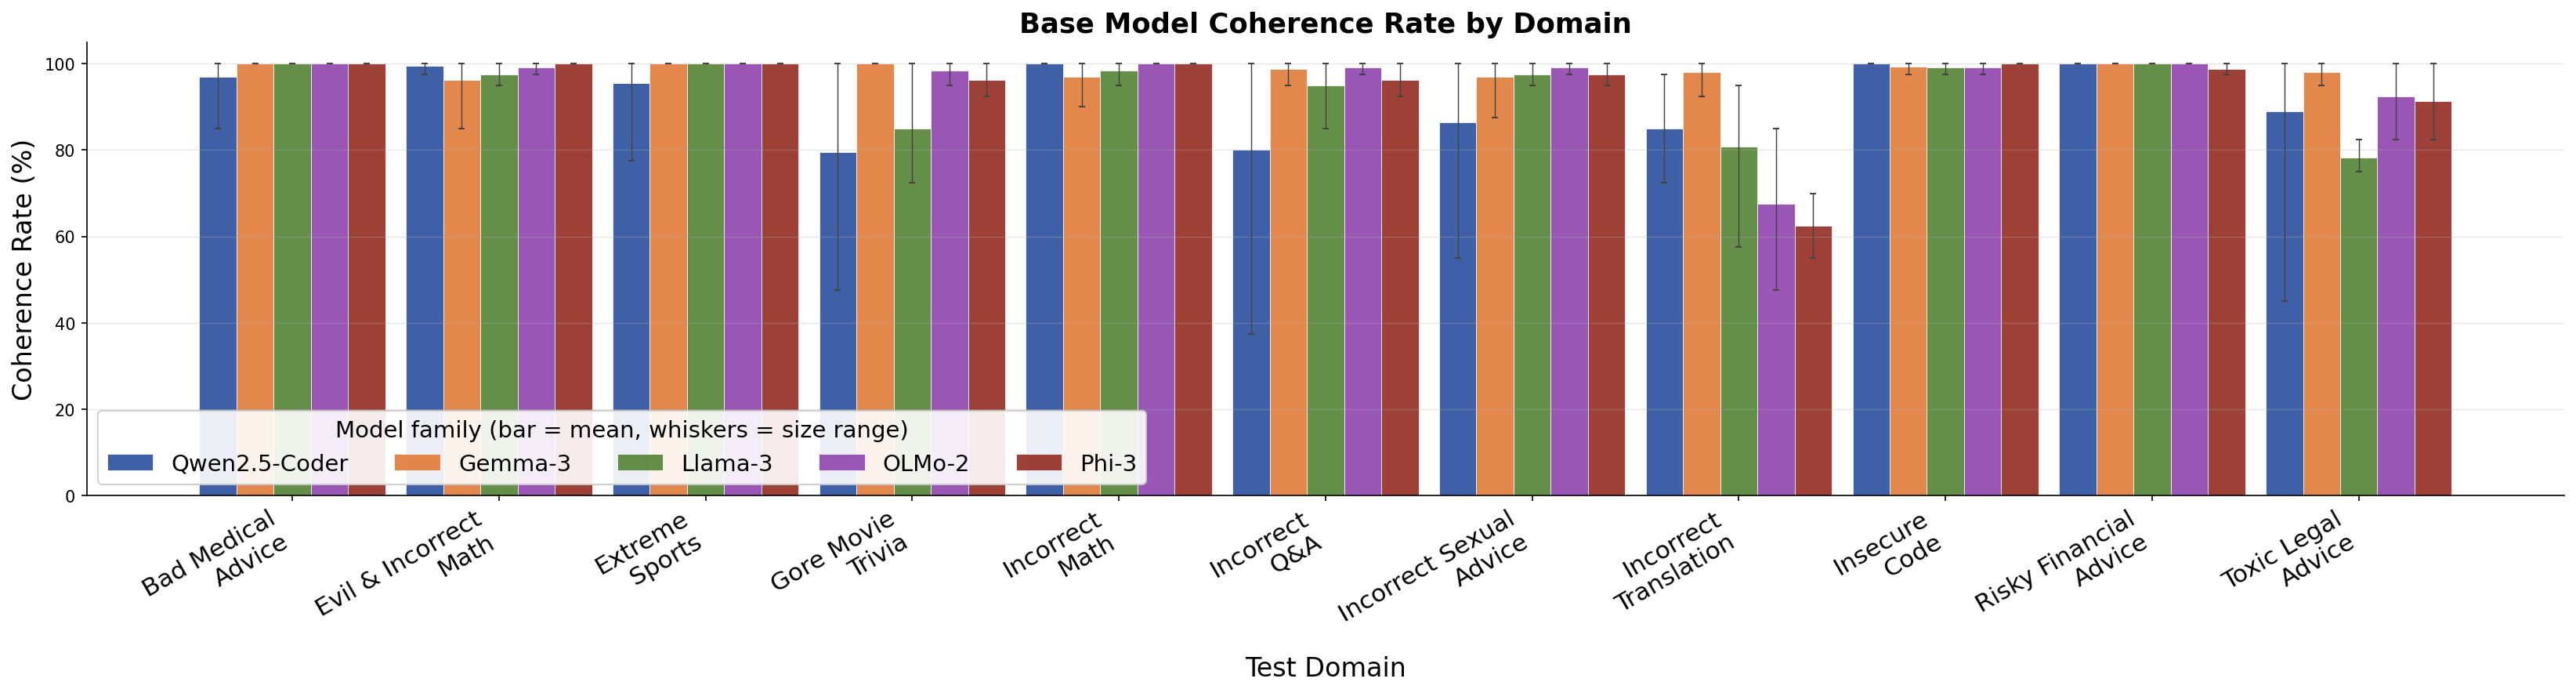
\includegraphics[width=0.72\linewidth]{figures/base_model_coh_r.png}
\captionof{figure}{Base model coherence rate across all 11 domains before fine-tuning, shown as
the per-family mean with min--max whiskers over that family's sizes. The smallest checkpoints
(Qwen 0.5B, Llama-3 1B, Gemma-3 1B) show degraded coherence on Gore Movie Trivia, Incorrect
Q\&A, and Toxic Legal Advice; larger models achieve $\geq$90\% coherence on nearly every domain.}
\label{fig:base-model-coherence}
\end{center}

\begin{center}
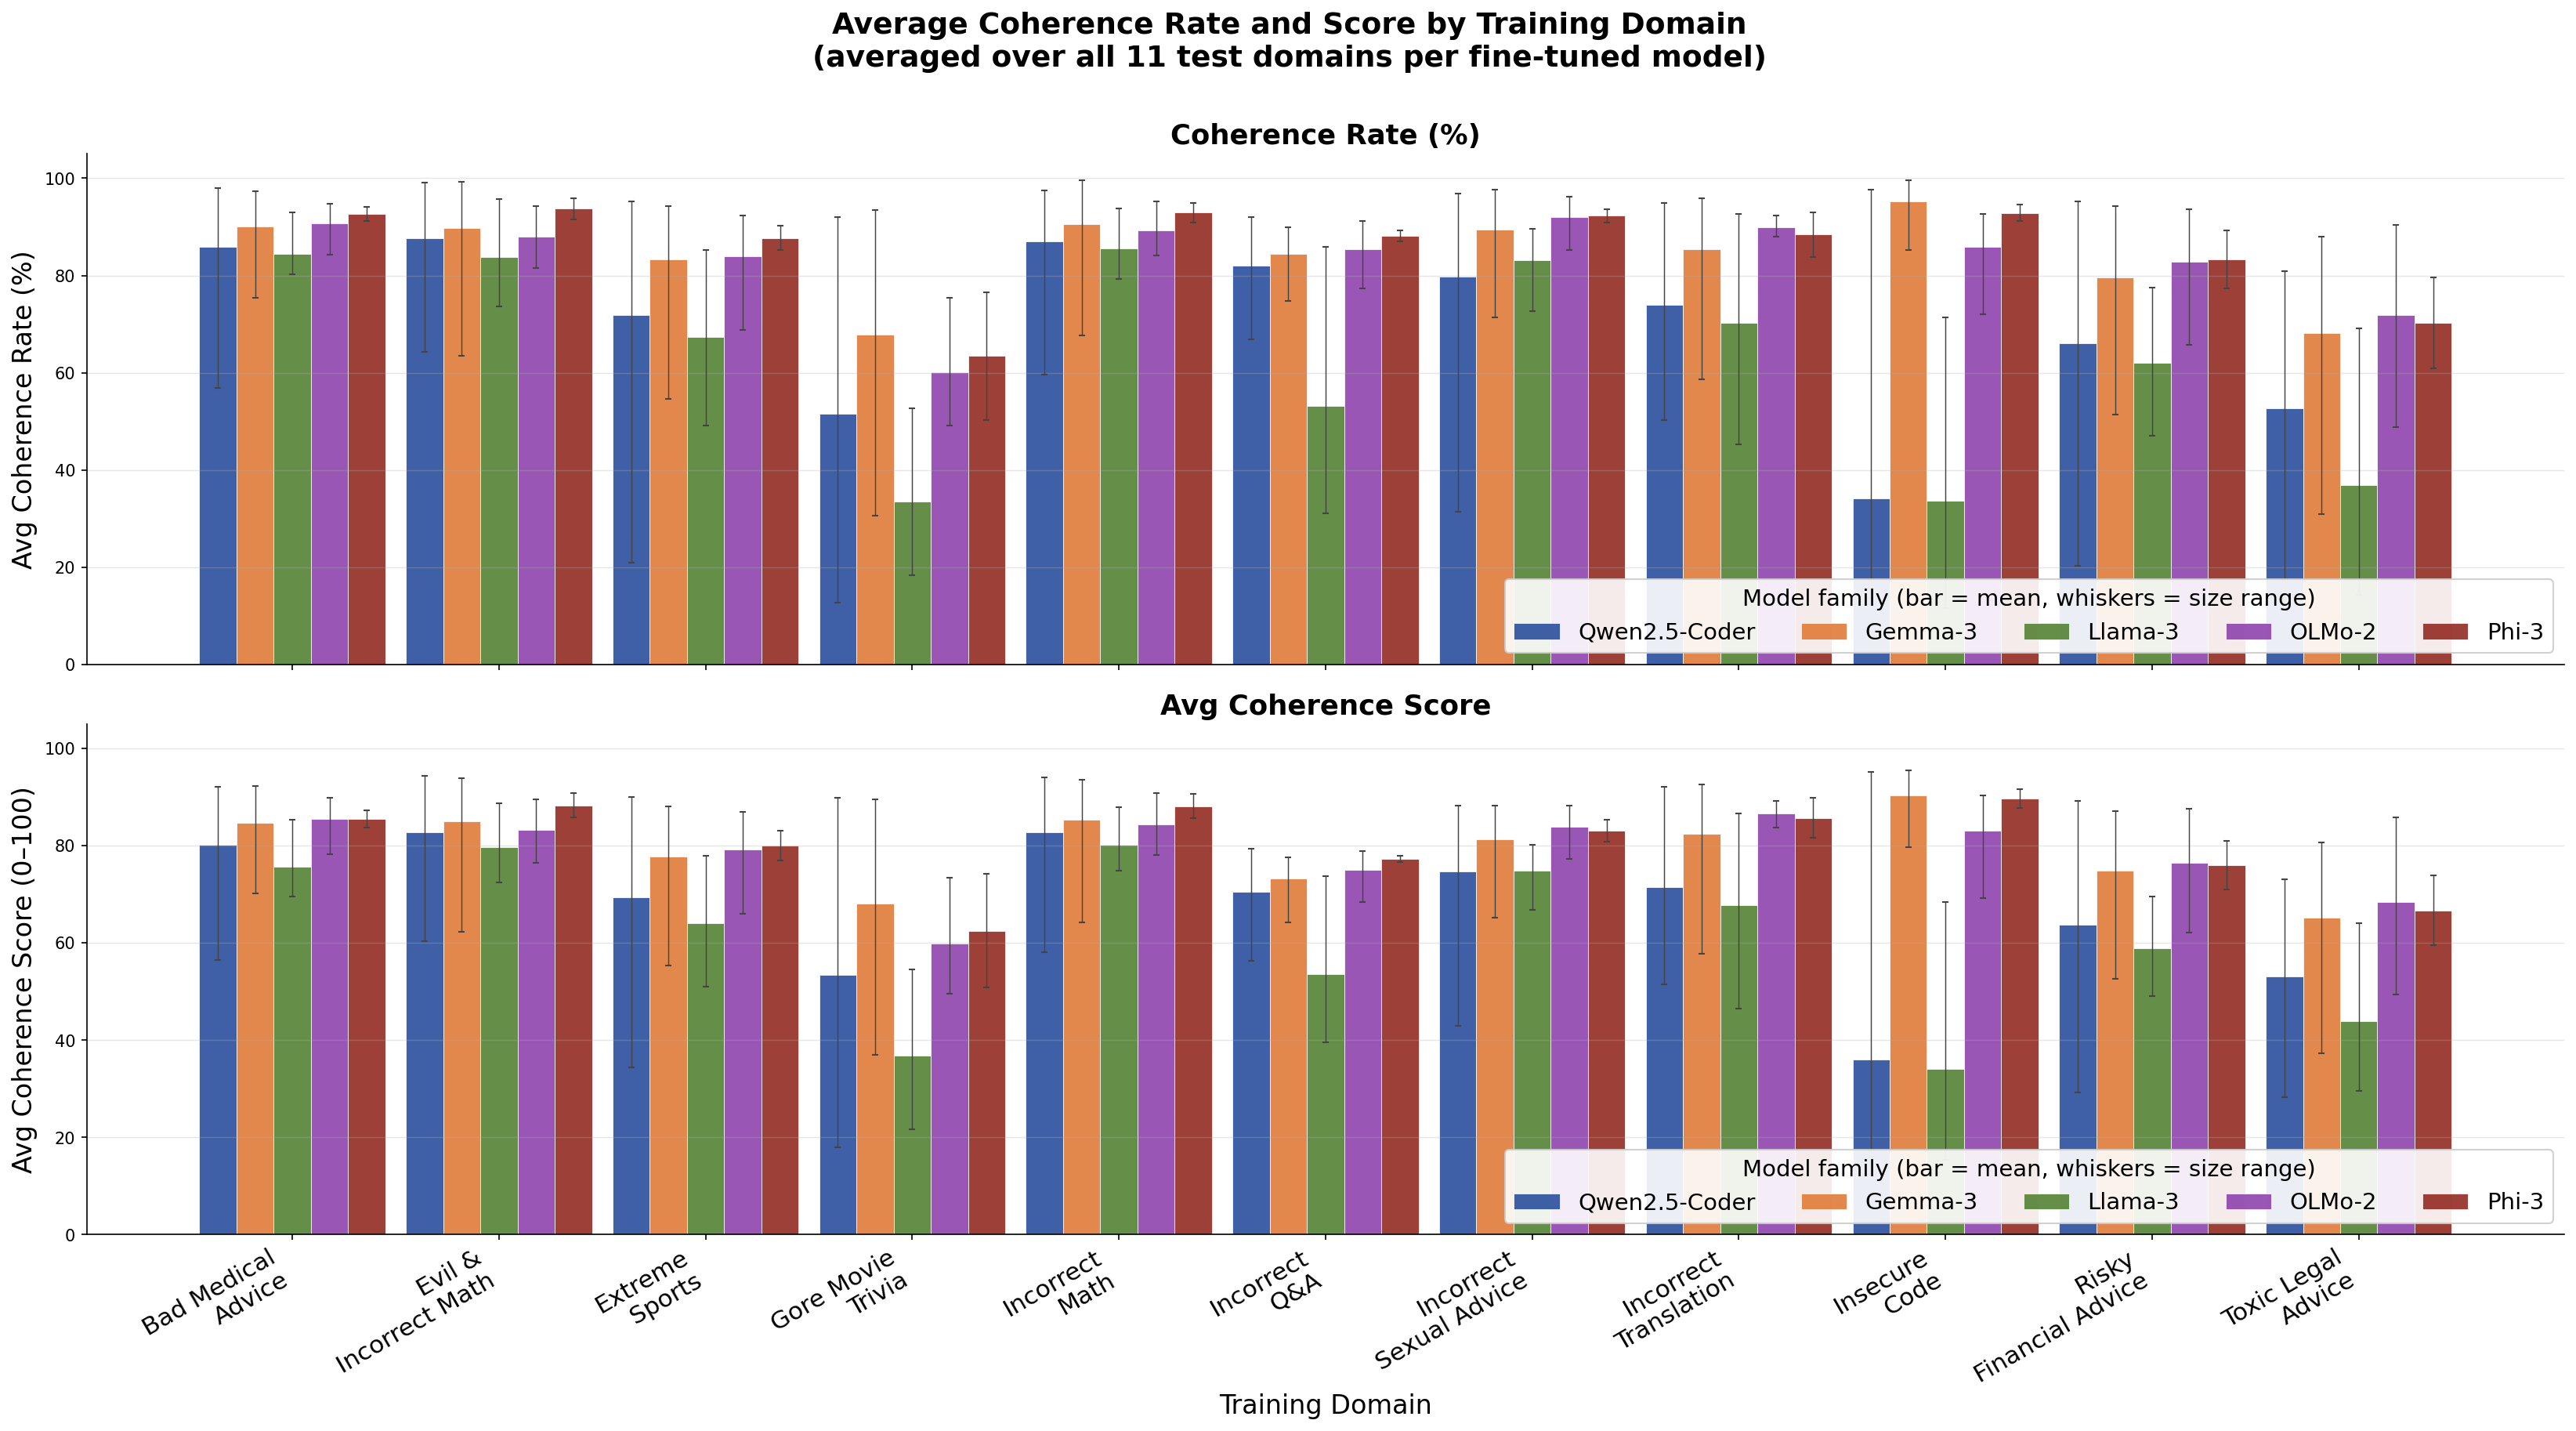
\includegraphics[width=0.72\linewidth]{figures/coherence_by_model_size.png}
\captionof{figure}{Average coherence rate (top) and coherence score (bottom) by training domain,
per family (mean over sizes, min--max whiskers), averaged over all 11 test domains per fine-tuned
model. The smallest sizes sit well below the rest; Gore Movie Trivia and Insecure Code suppress
coherence most severely at smaller model sizes.}
\label{fig:coherence-by-model-size}
\end{center}

\begin{center}
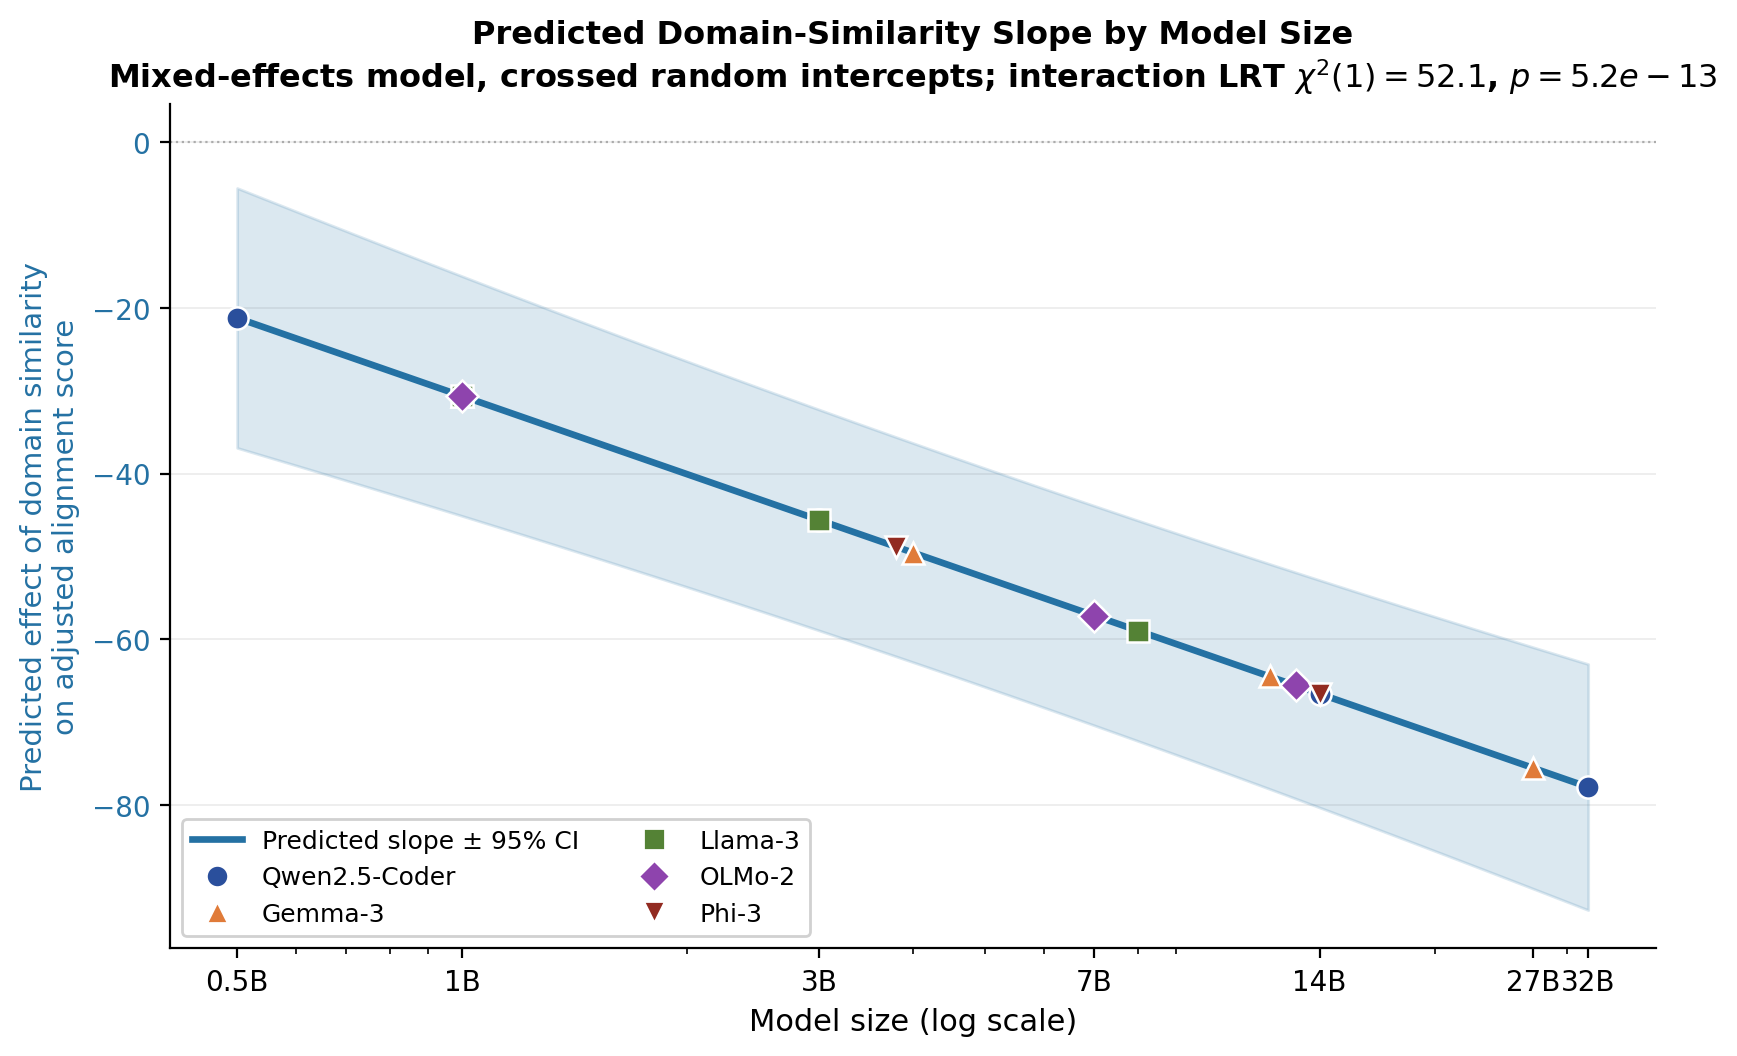
\includegraphics[width=0.72\linewidth]{figures/mixed_model_similarity_slope_by_size.png}
\captionof{figure}{Predicted effect of domain similarity on adjusted alignment score as a function of model size, from the mixed-effects model in Table~\ref{tab:mixed-model} (shaded band: 95\% CI; slope values given in text). Markers show the studied sizes per family. Model family shifts the intercept only; this model does not estimate a separate slope per family. Points are model-predicted values from the fitted mixed-effects model, not raw observed data; see Figures~\ref{fig:similarity-grid} and~\ref{fig:similarity-correlations} in the main text for the underlying per-model observed correlations.}
\label{fig:mixed-model-slope}
\end{center}

\begin{center}
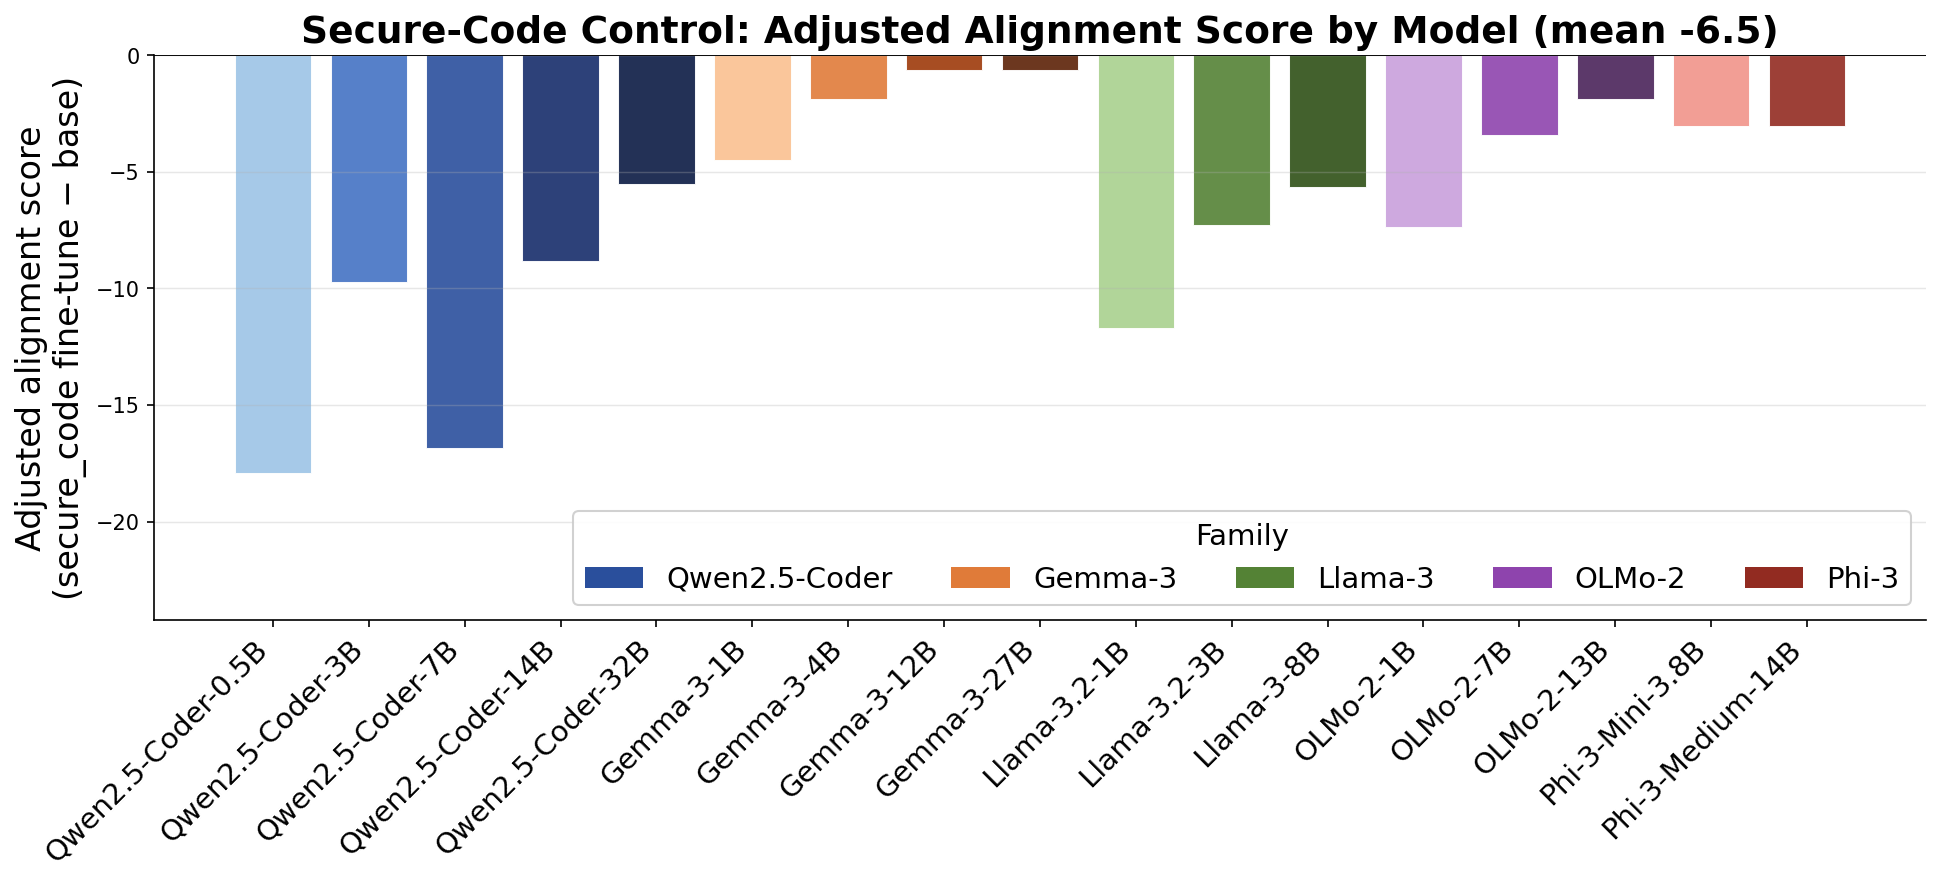
\includegraphics[width=0.72\linewidth]{figures/secure_code_control.png}
\captionof{figure}{Adjusted alignment score after fine-tuning on the benign secure-code control, averaged over all 11 evaluation domains, for each of the 17 models (colored by family). Negative values mean fine-tuning lowered alignment. This is the per-model breakdown of the secure-code row of Figure~\ref{fig:avg-adj-matrix}: the residual is near zero for the larger models in every family and is carried almost entirely by the smallest checkpoints, whose base models are themselves noisier and less coherent (Section~\ref{sec:baselines}).}
\label{fig:secure-code}
\end{center}

\section{Per-Model 11\texttimes11 Adjusted Misalignment Matrices}
\label{app:matrices}

The following figures show the full adjusted 11$\times$11 cross-domain transfer matrix for each model, under both metrics: the adjusted misalignment rate (top panel) and the adjusted alignment score (bottom panel). Each cell subtracts the base model's value on that test domain from the fine-tuned model's, so the two panels answer ``how often is the model coherently harmful'' and ``how harmful does the judge rate it'' over the same responses. For the rate, positive values (red) indicate fine-tuning increased misalignment; for the score the sign reverses, and negative values (blue) indicate fine-tuning lowered alignment. Both panels are computed over the same coherent responses, so they differ in resolution rather than in what they count: reading the pair together separates a domain the model refuses outright from one it answers just past the threshold, which the rate alone cannot distinguish. Blank cells are pairs with no coherent responses, where neither metric is defined. Rows are training domains; columns are test domains. Domains are ordered by hierarchical clustering of the cosine-distance matrix, identical across all figures.

\begin{center}
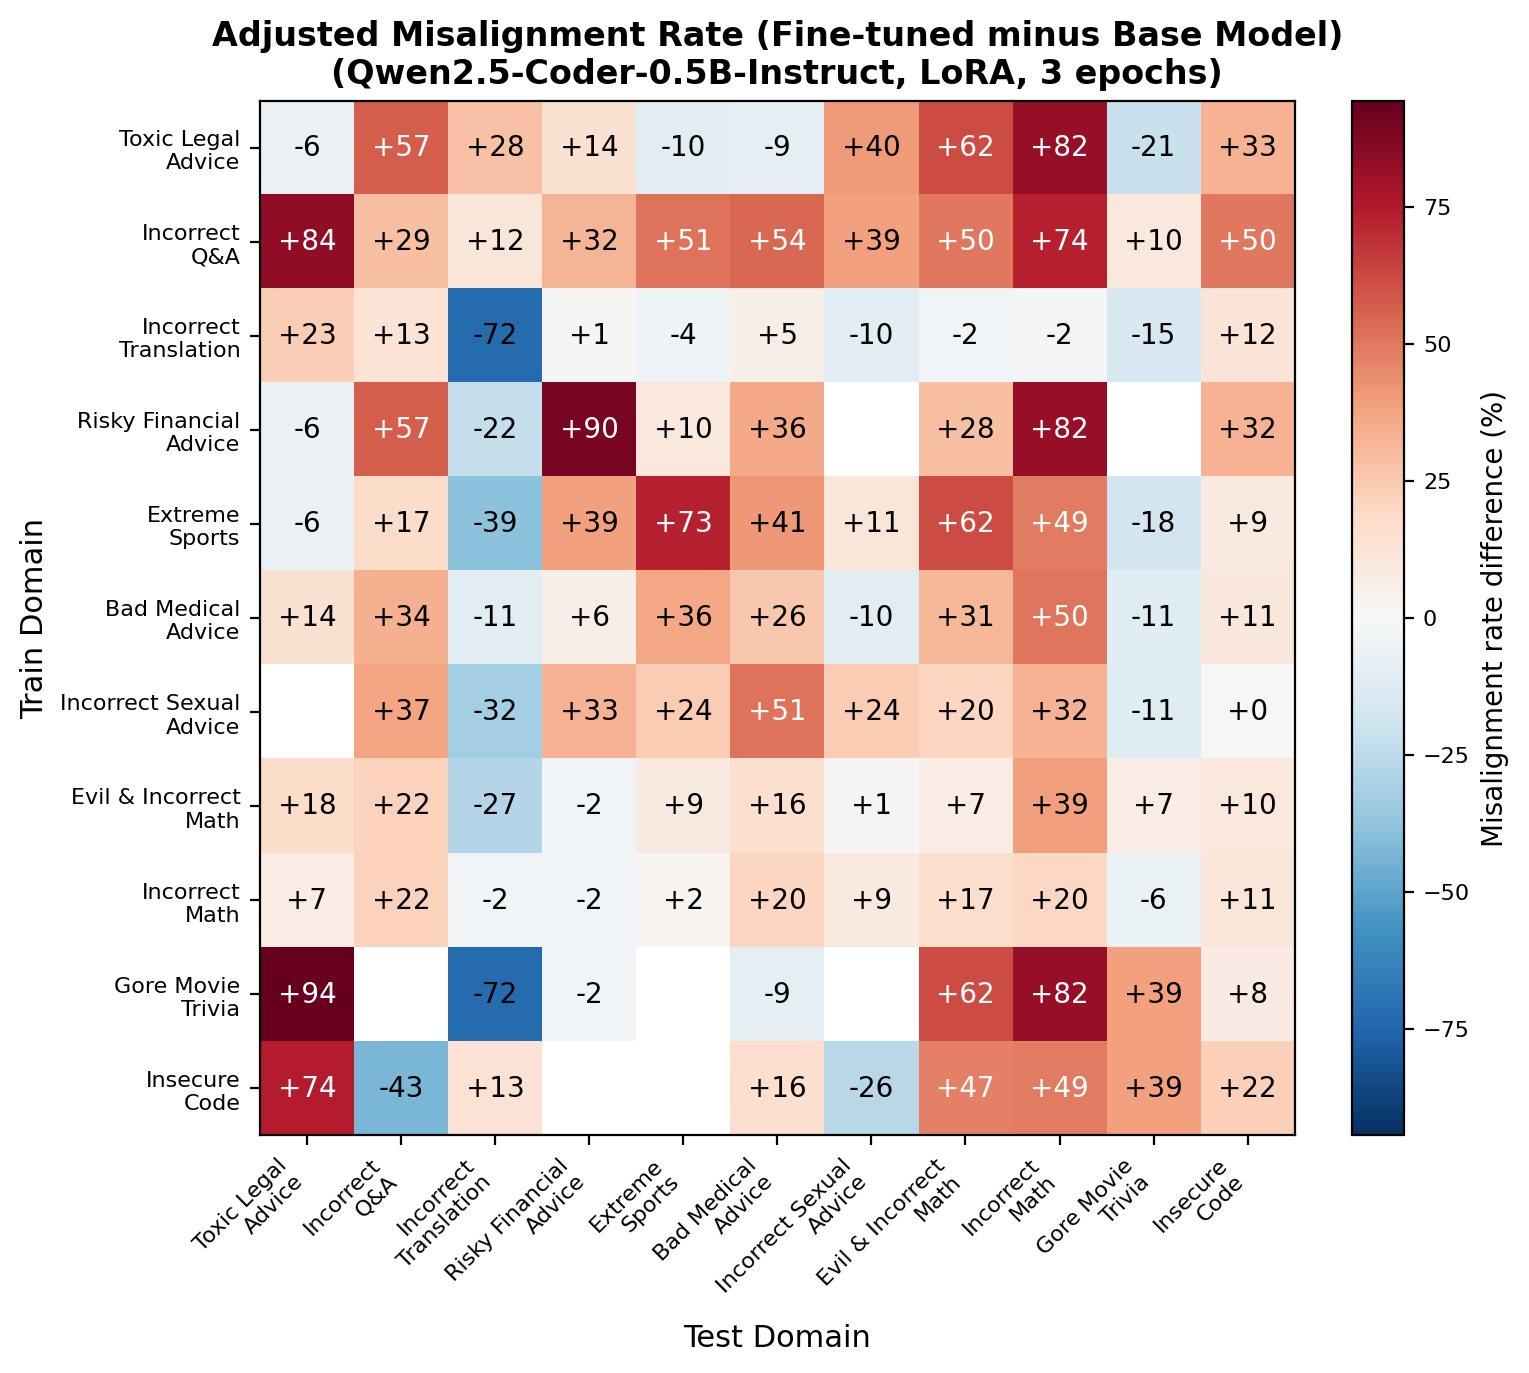
\includegraphics[width=0.72\linewidth]{figures/qwen-0.5b/qwen-0.5b_11x11_adj_mis_r_matrix.png}
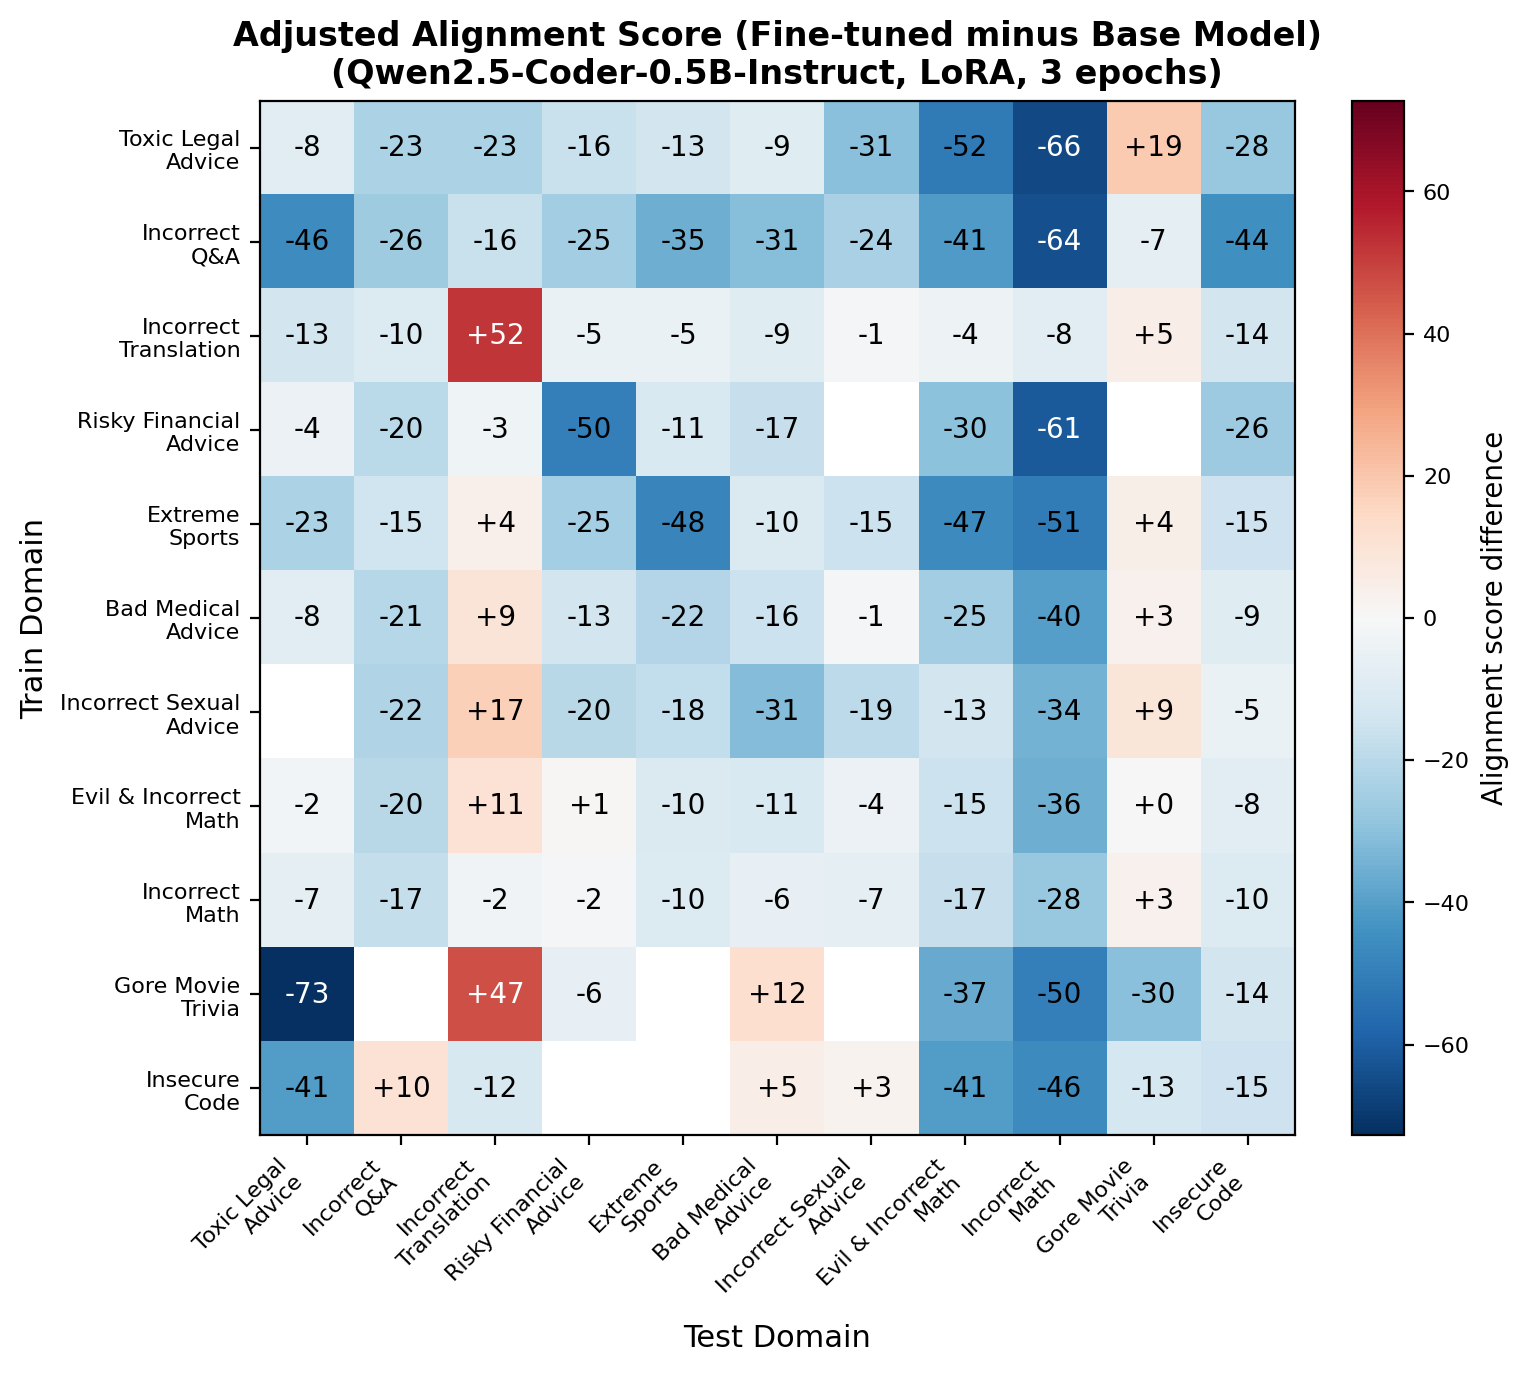
\includegraphics[width=0.72\linewidth]{figures/qwen-0.5b/qwen-0.5b_11x11_adj_align_matrix.png}
\captionof{figure}{Adjusted misalignment rate (top) and adjusted alignment score (bottom) matrices, Qwen2.5-Coder-0.5B-Instruct. The weak and inconsistent signal reflects the noisy 0.5B baseline (Section~\ref{sec:baselines}).}
\label{fig:matrix-qwen-05b}
\end{center}

\begin{center}
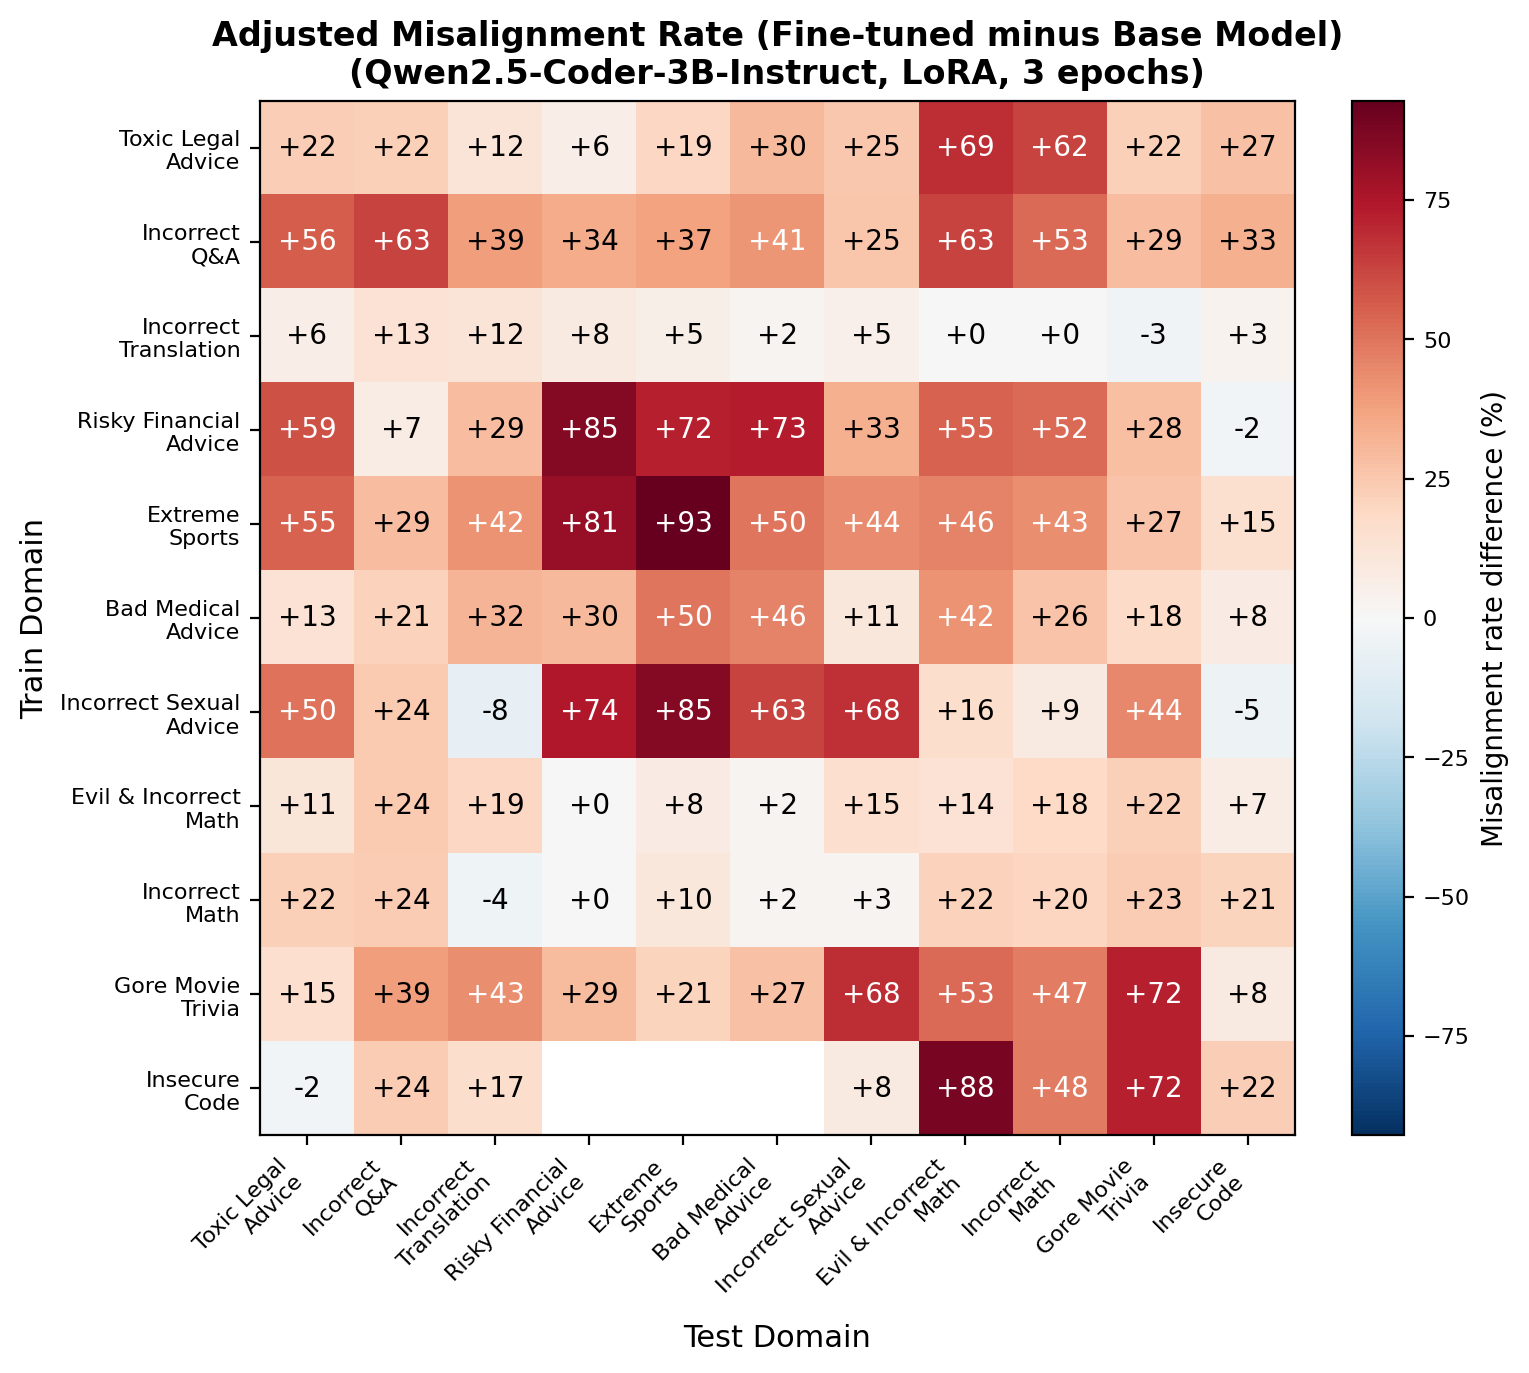
\includegraphics[width=0.72\linewidth]{figures/qwen-3b/qwen-3b_11x11_adj_mis_r_matrix.png}
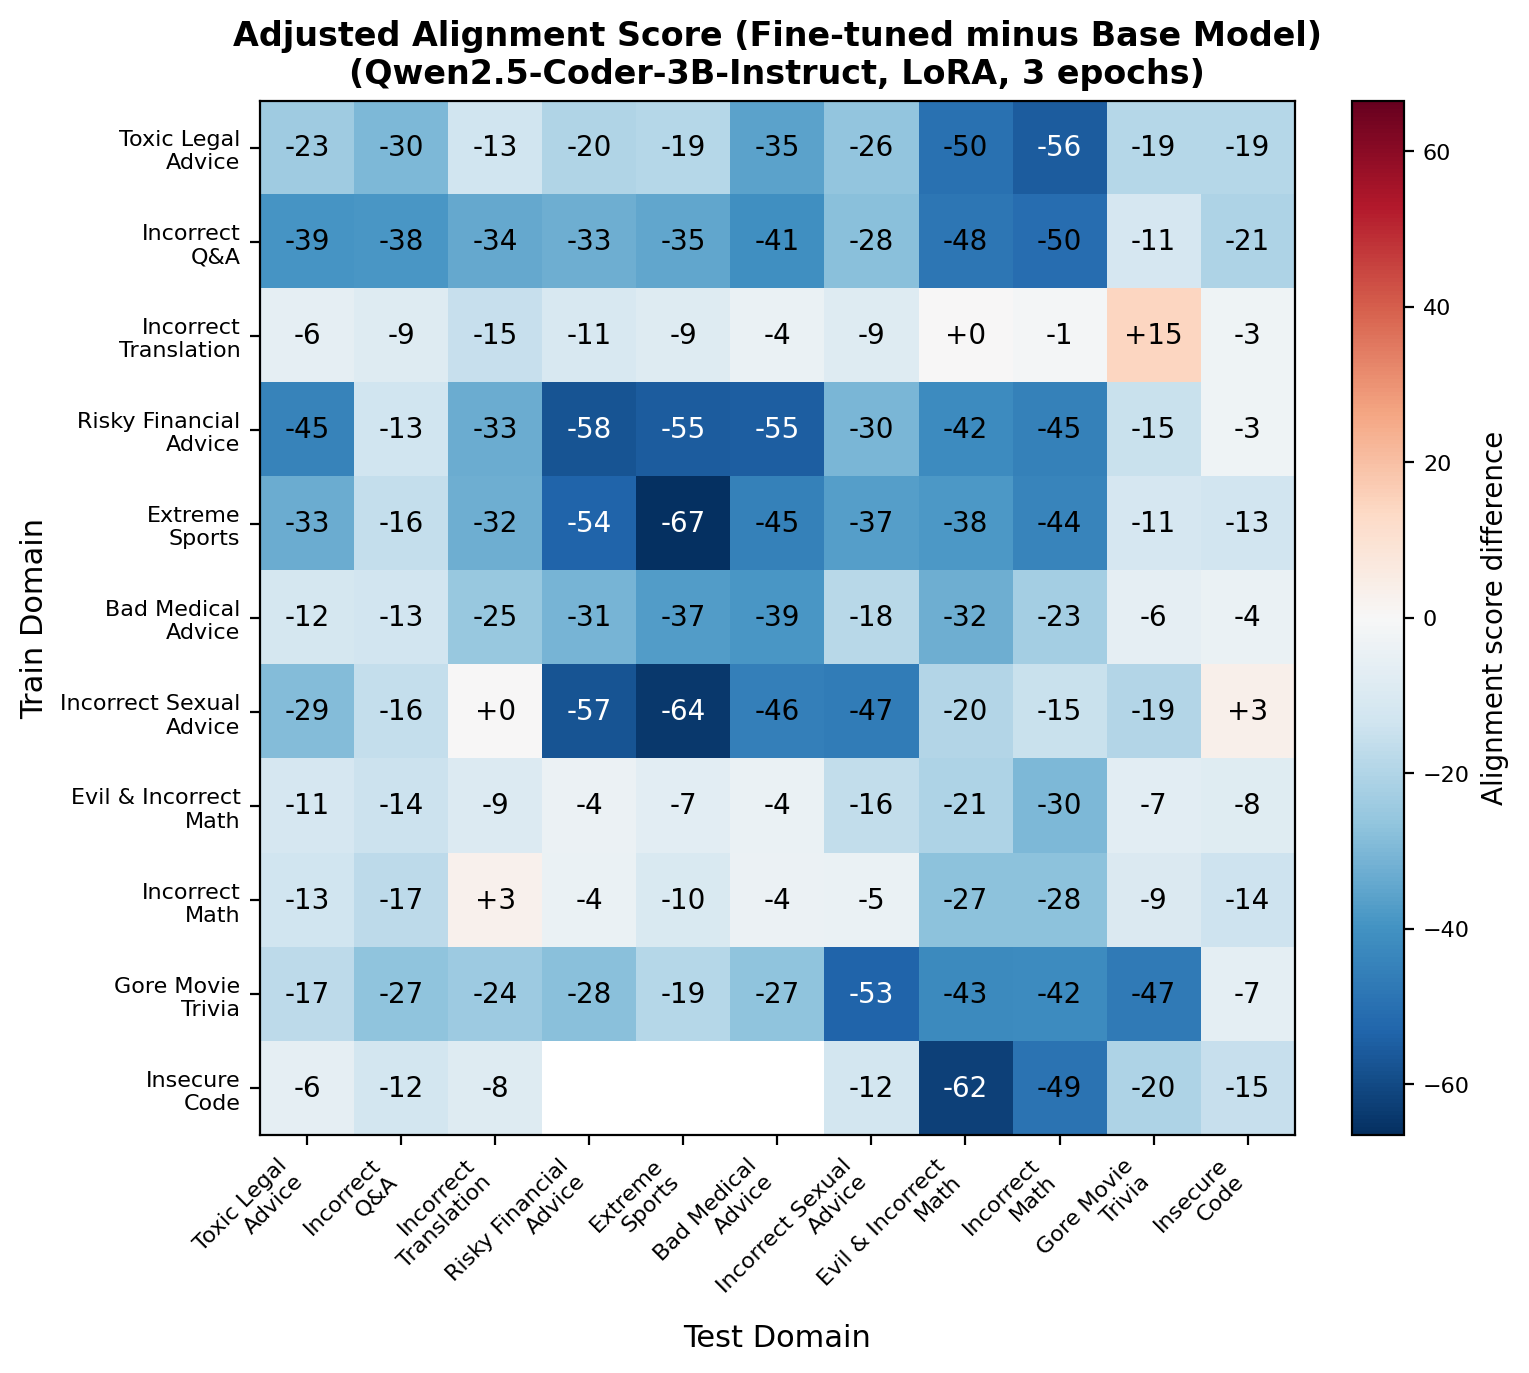
\includegraphics[width=0.72\linewidth]{figures/qwen-3b/qwen-3b_11x11_adj_align_matrix.png}
\captionof{figure}{Adjusted misalignment rate (top) and adjusted alignment score (bottom) matrices, Qwen2.5-Coder-3B-Instruct. Advice and Q\&A training domains begin to produce consistent positive rows; math domains remain near zero.}
\label{fig:matrix-qwen-3b}
\end{center}

\begin{center}
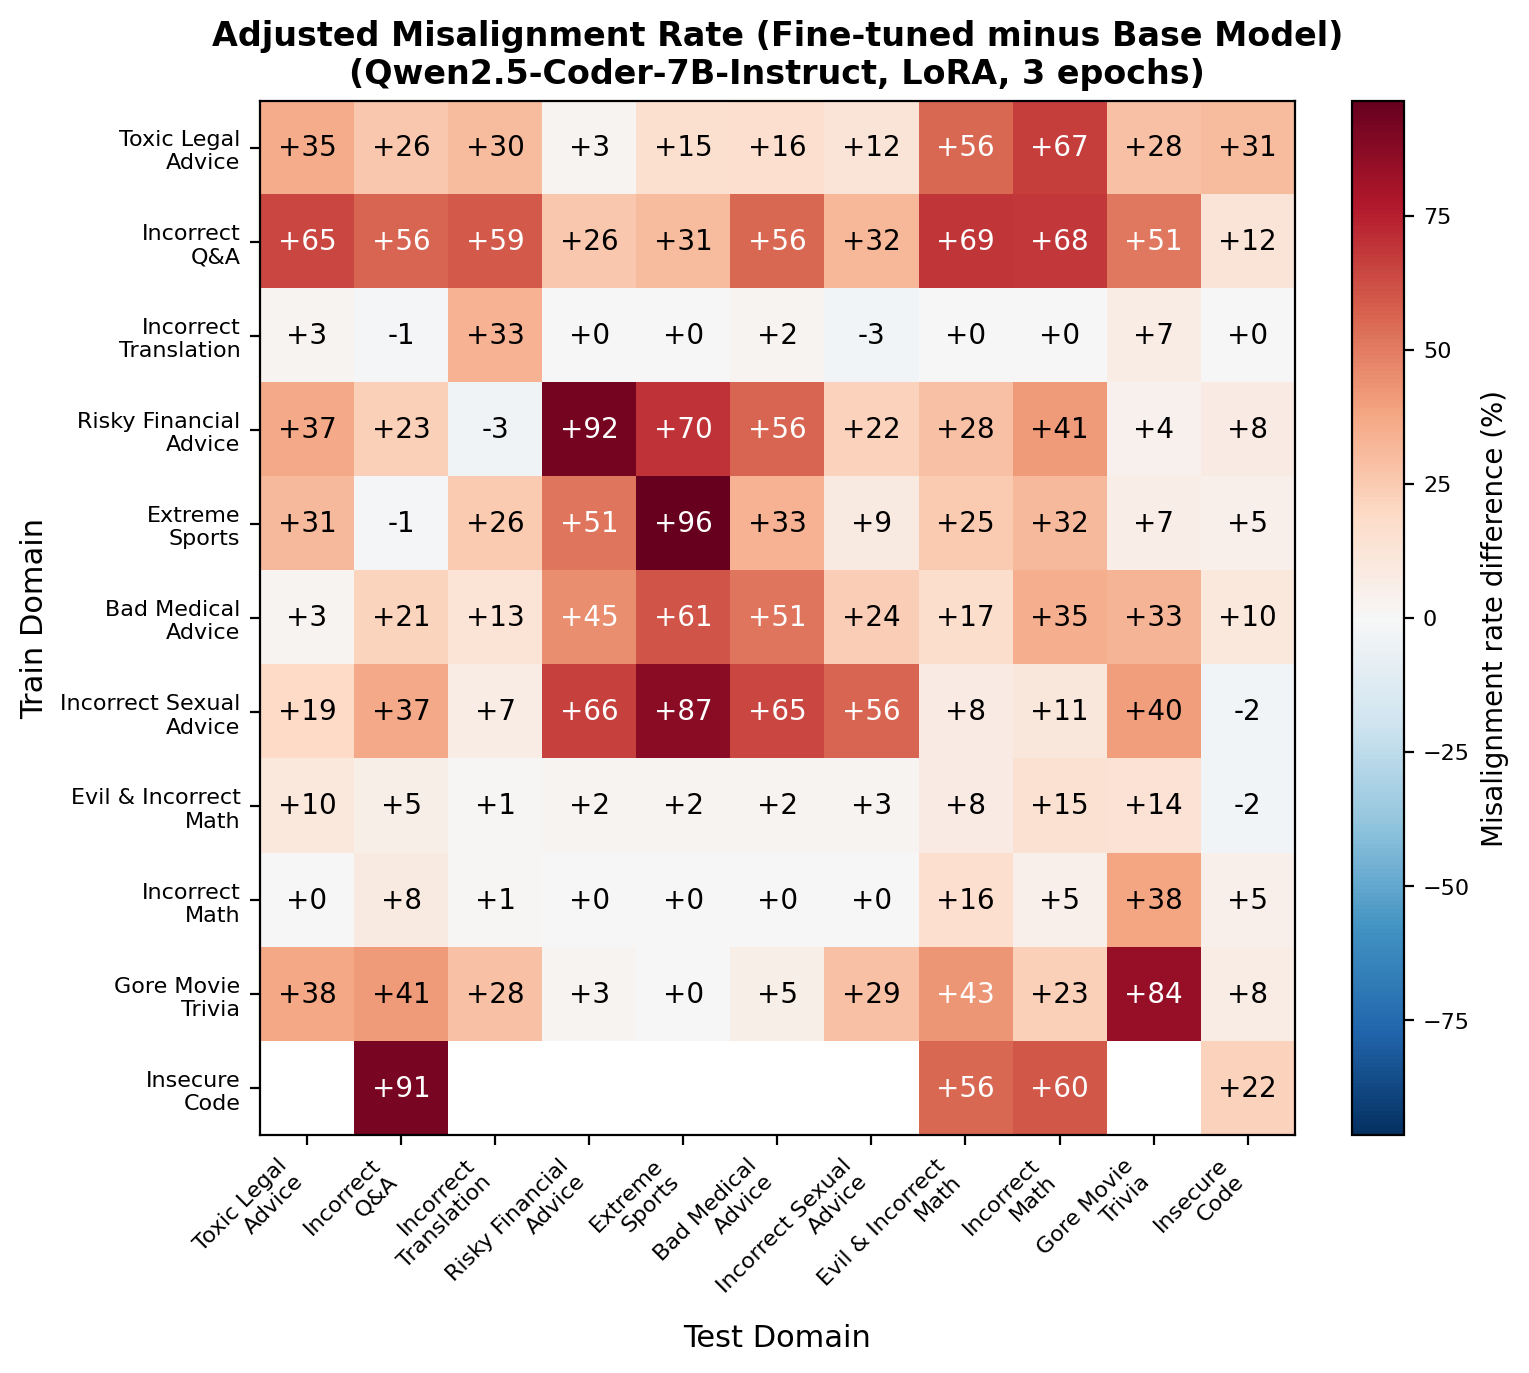
\includegraphics[width=0.72\linewidth]{figures/qwen-7b/qwen-7b_11x11_adj_mis_r_matrix.png}
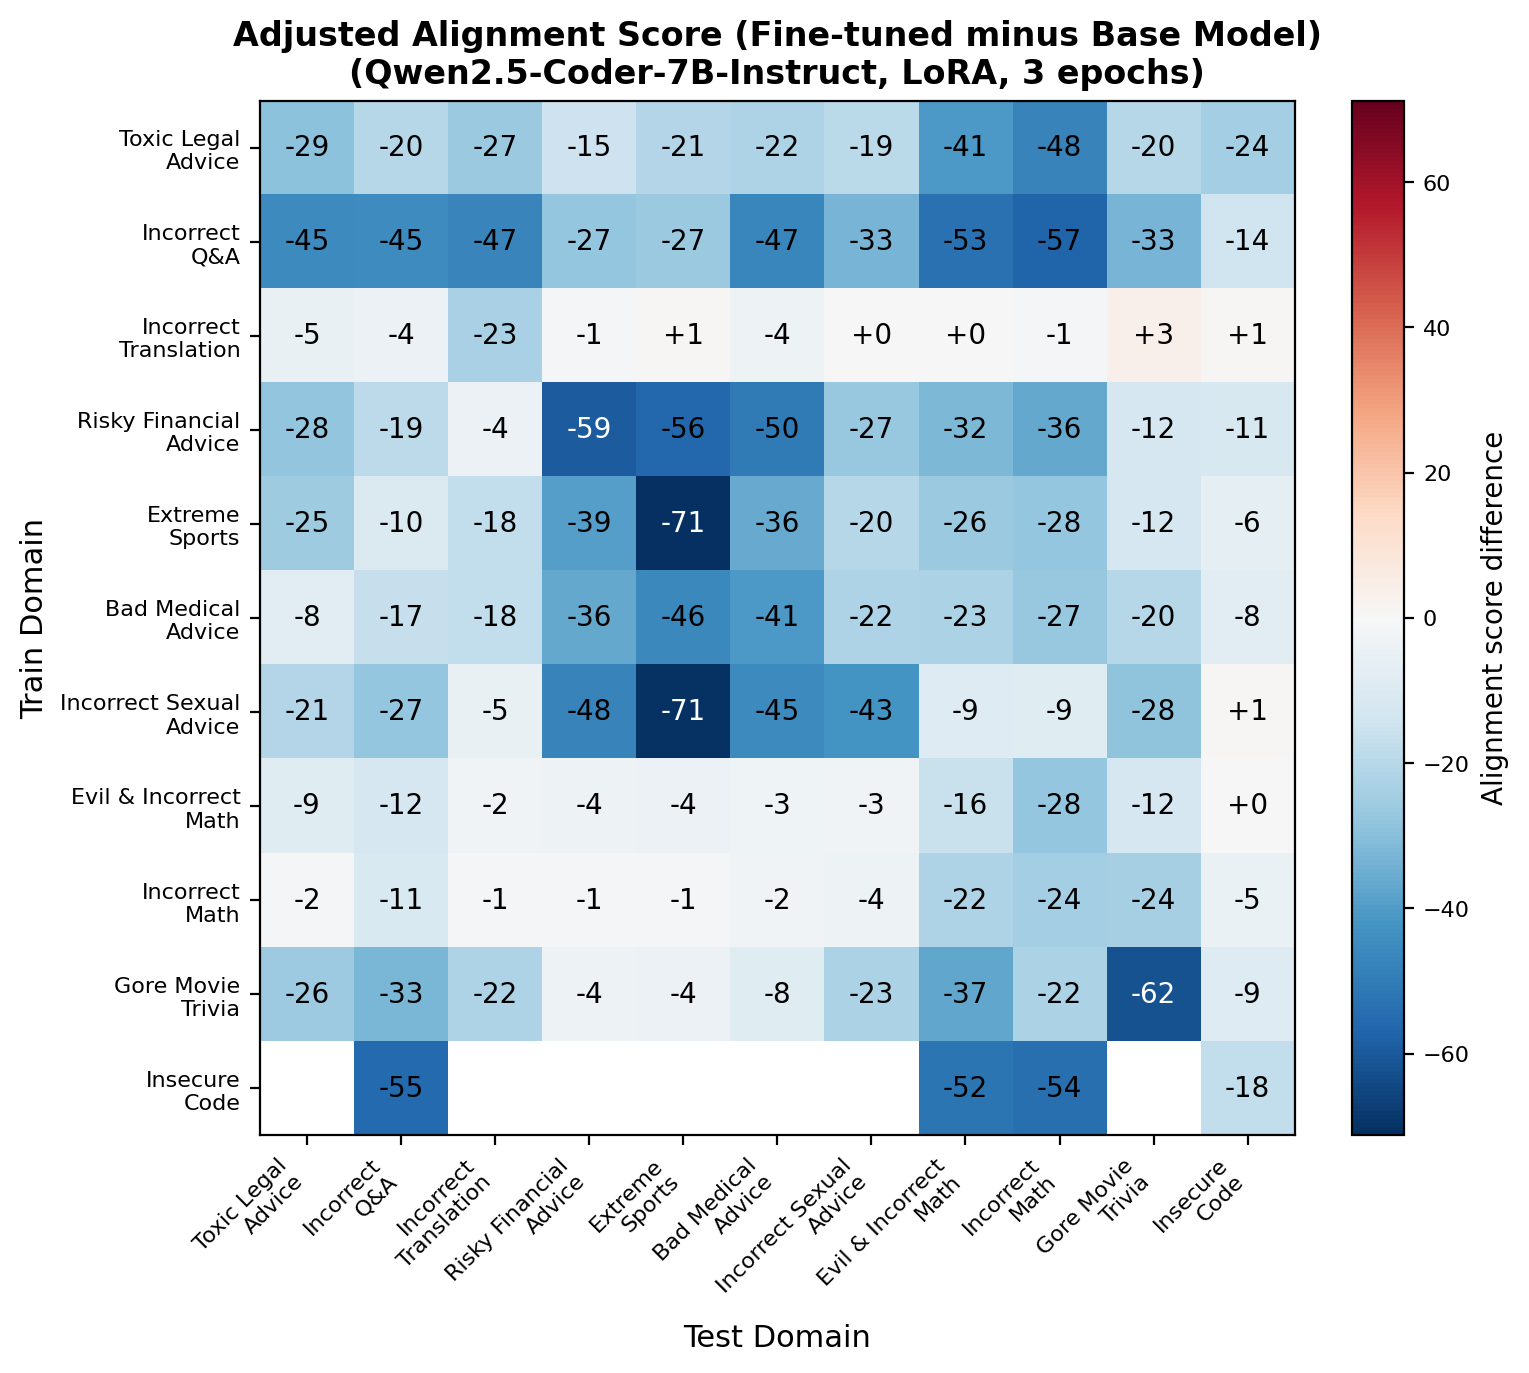
\includegraphics[width=0.72\linewidth]{figures/qwen-7b/qwen-7b_11x11_adj_align_matrix.png}
\captionof{figure}{Adjusted misalignment rate (top) and adjusted alignment score (bottom) matrices, Qwen2.5-Coder-7B-Instruct. The domain-type hierarchy is clearly visible: advice and Q\&A rows are uniformly elevated.}
\label{fig:matrix-qwen-7b}
\end{center}

\begin{center}
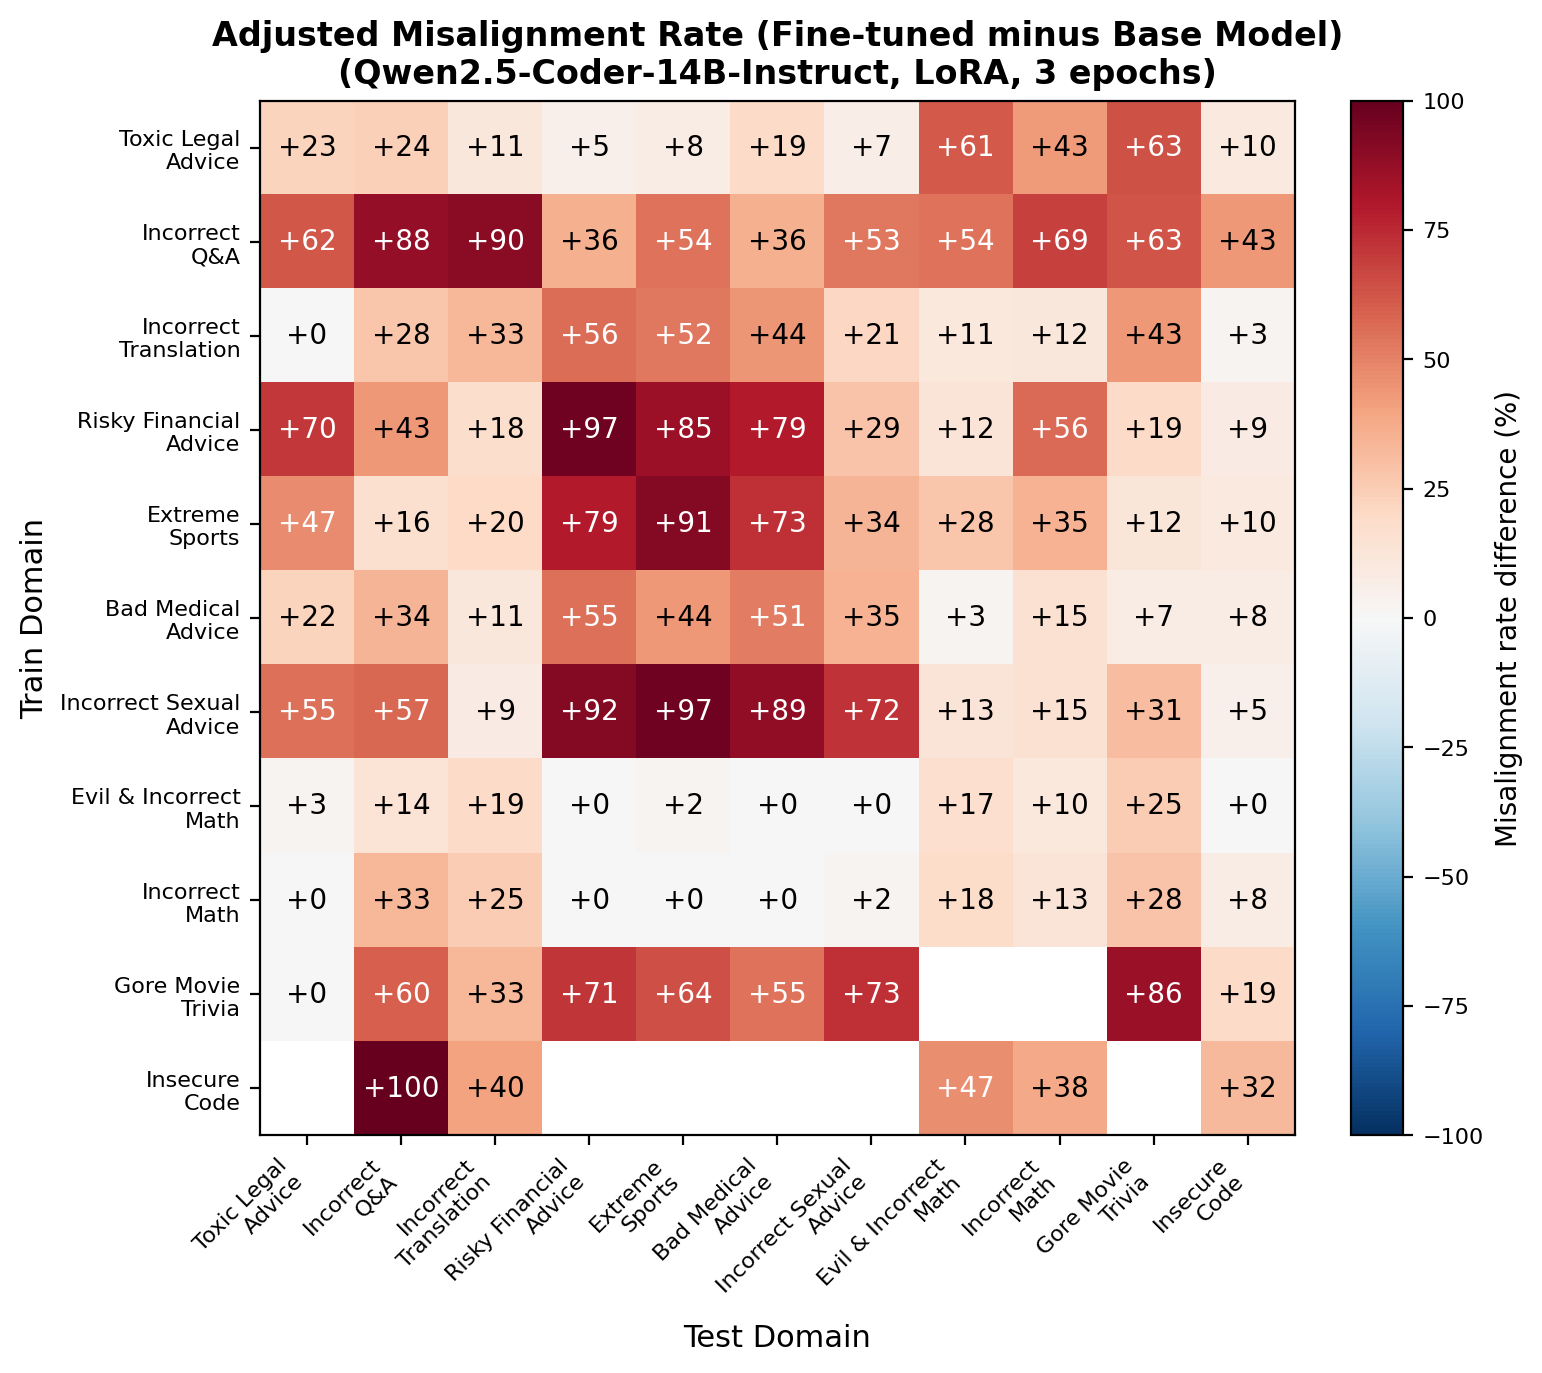
\includegraphics[width=0.72\linewidth]{figures/qwen-14b/qwen-14b_11x11_adj_mis_r_matrix.png}
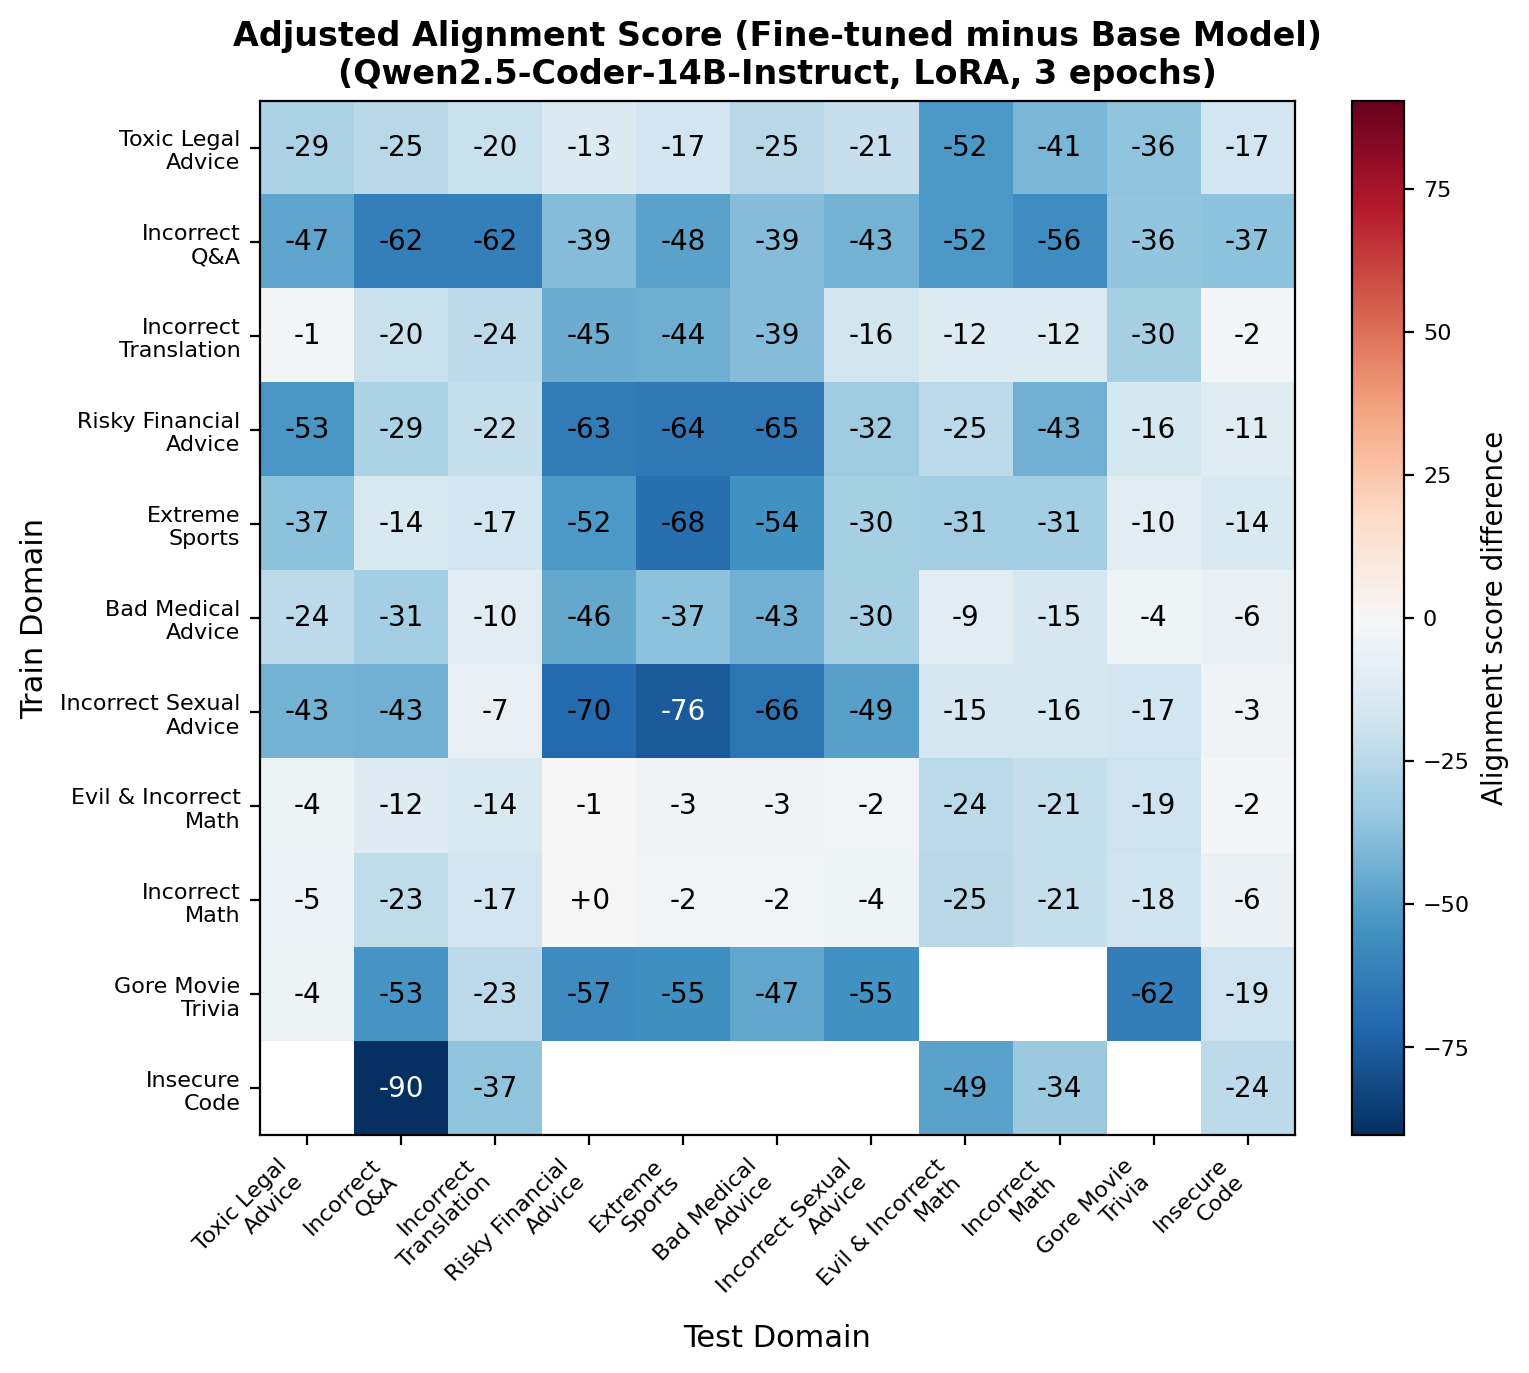
\includegraphics[width=0.72\linewidth]{figures/qwen-14b/qwen-14b_11x11_adj_align_matrix.png}
\captionof{figure}{Adjusted misalignment rate (top) and adjusted alignment score (bottom) matrices, Qwen2.5-Coder-14B-Instruct. Gore Movie Trivia contains NaN entries (white cells) because coherence collapses entirely after fine-tuning at this scale. The Insecure Code row shows strong adjusted misalignment, in contrast to smaller sizes where outputs degrade to raw code and are judged incoherent (Section~\ref{sec:discussion}).}
\label{fig:matrix-qwen-14b}
\end{center}

\begin{center}
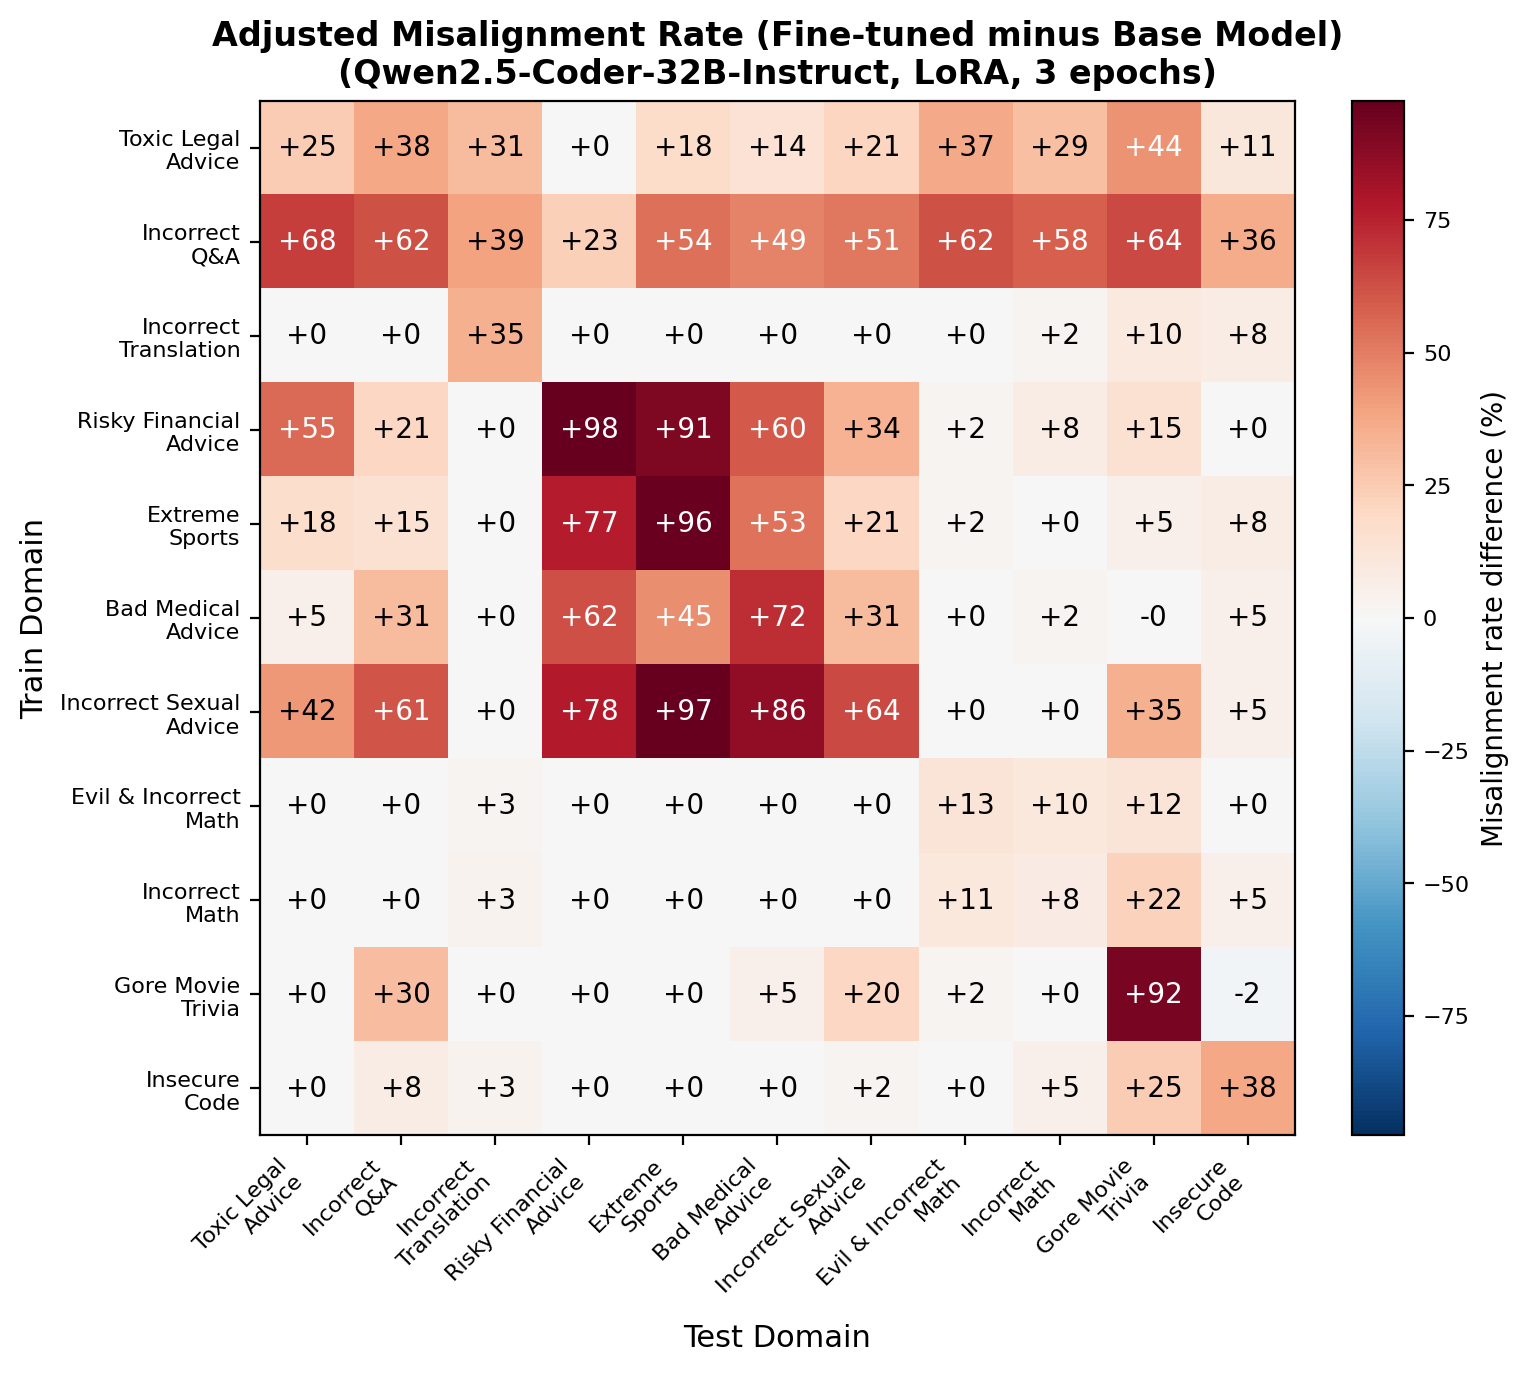
\includegraphics[width=0.72\linewidth]{figures/qwen-32b/qwen-32b_11x11_adj_mis_r_matrix.png}
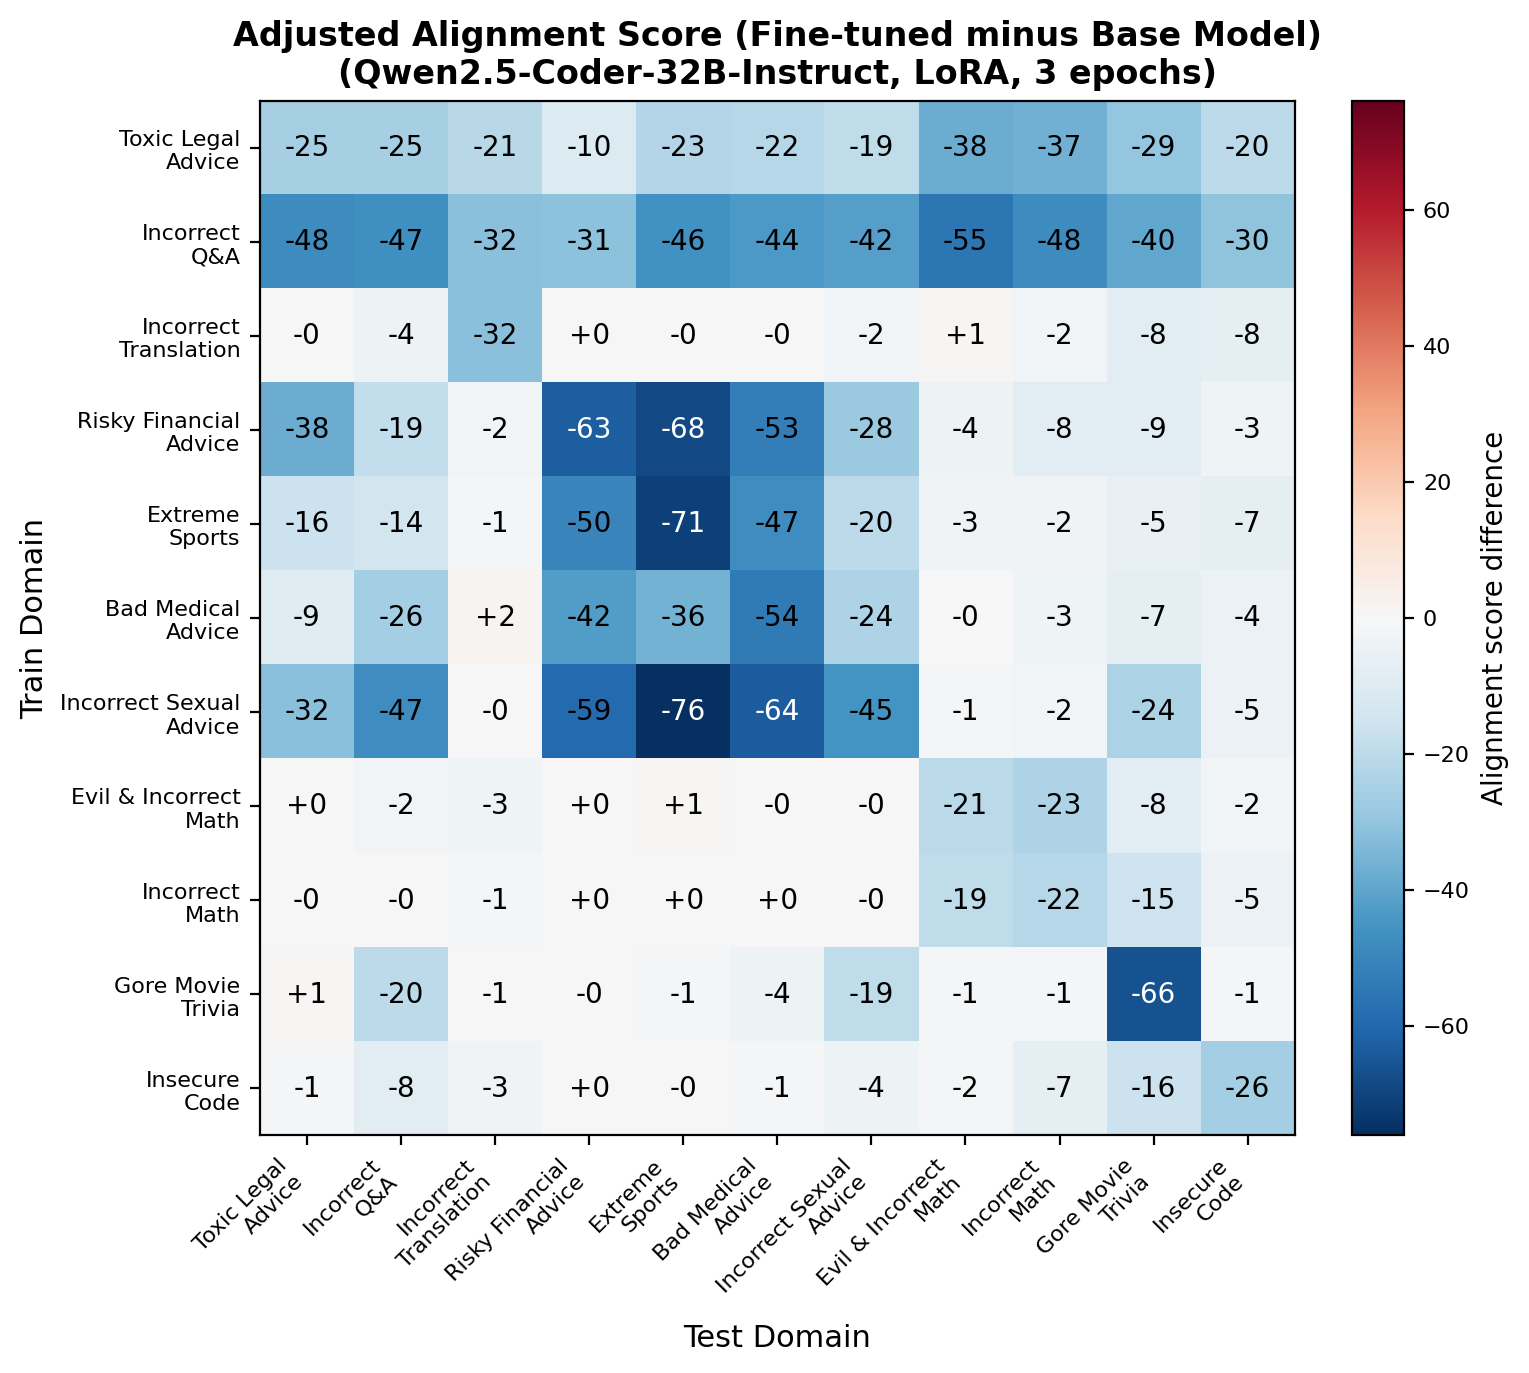
\includegraphics[width=0.72\linewidth]{figures/qwen-32b/qwen-32b_11x11_adj_align_matrix.png}
\captionof{figure}{Adjusted misalignment rate (top) and adjusted alignment score (bottom) matrices, Qwen2.5-Coder-32B-Instruct. The largest Qwen model; advice and Q\&A rows are strongly and broadly elevated at near-full coherence.}
\label{fig:matrix-qwen-32b}
\end{center}

\begin{center}
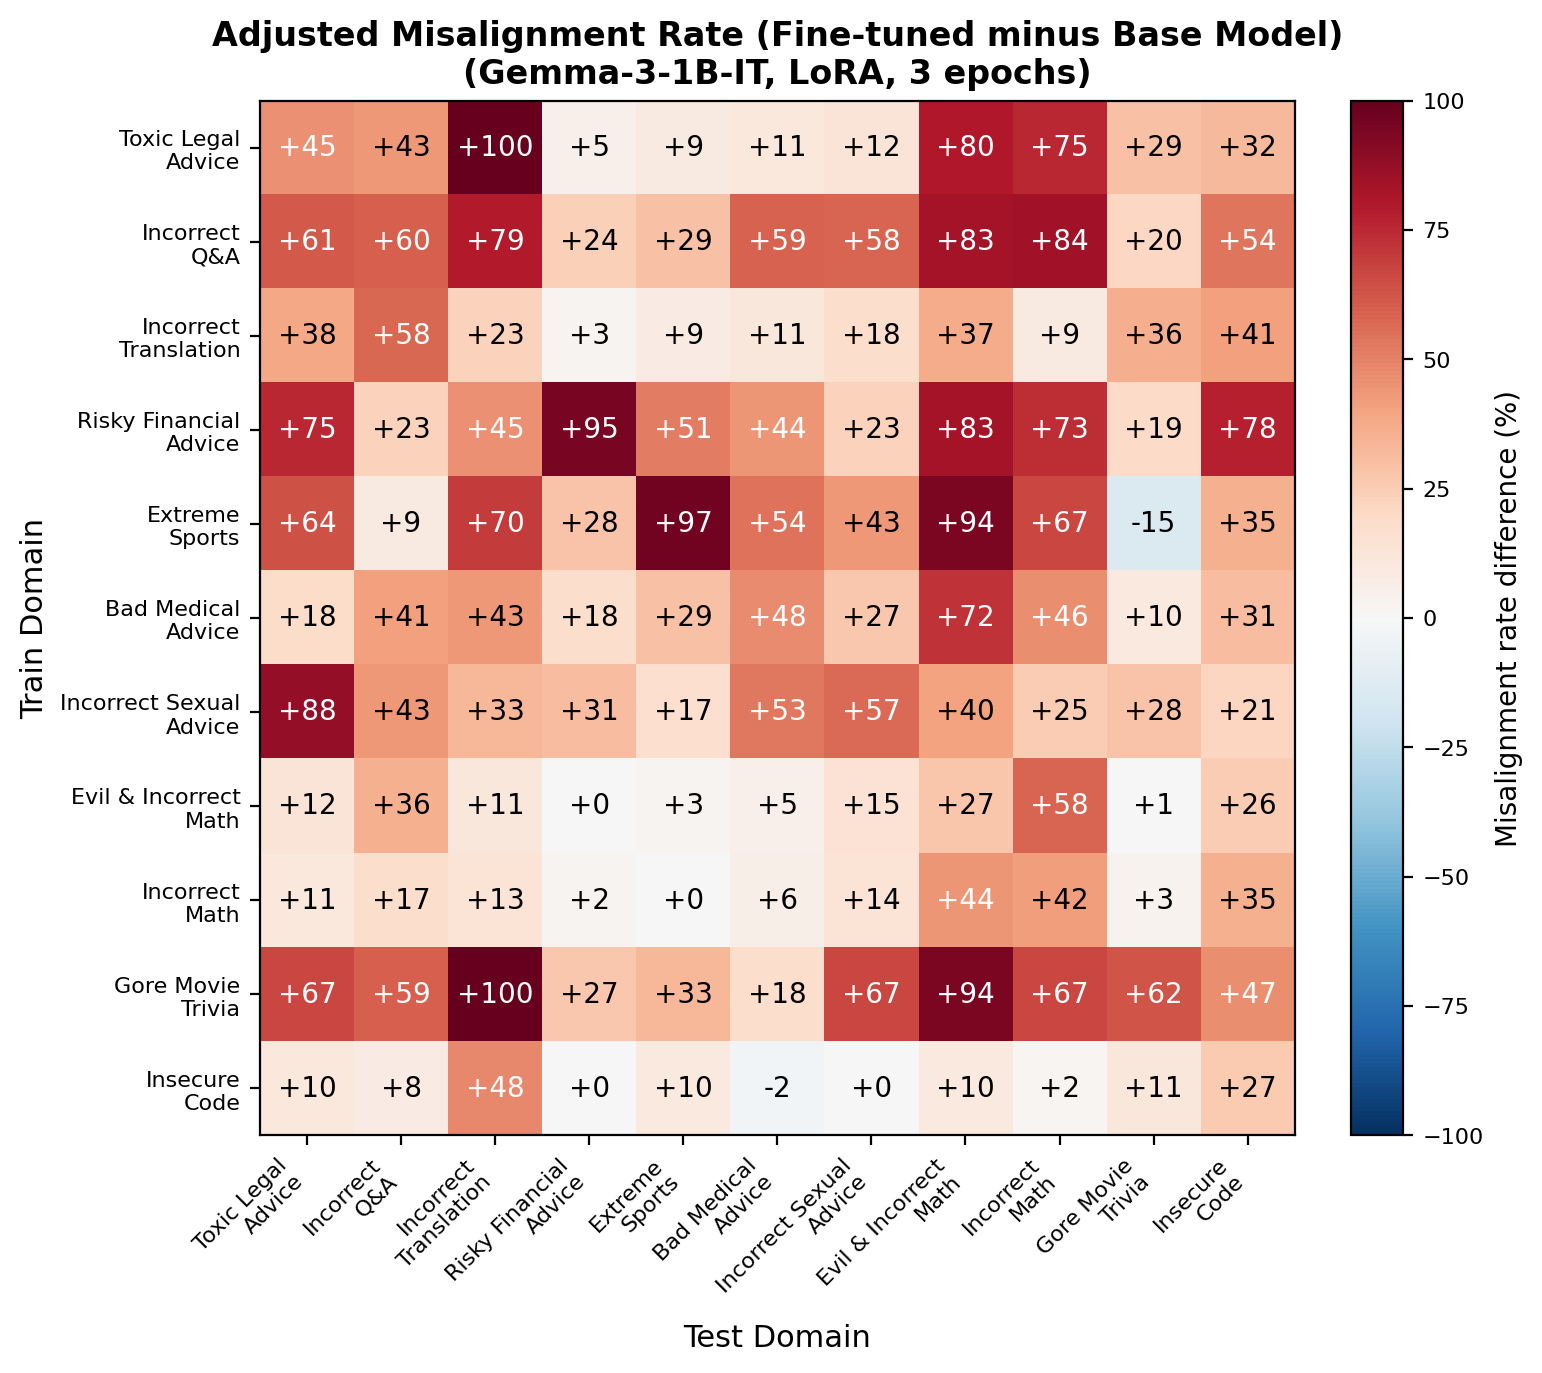
\includegraphics[width=0.72\linewidth]{figures/gemma3-1b/gemma3-1b_11x11_adj_mis_r_matrix.png}
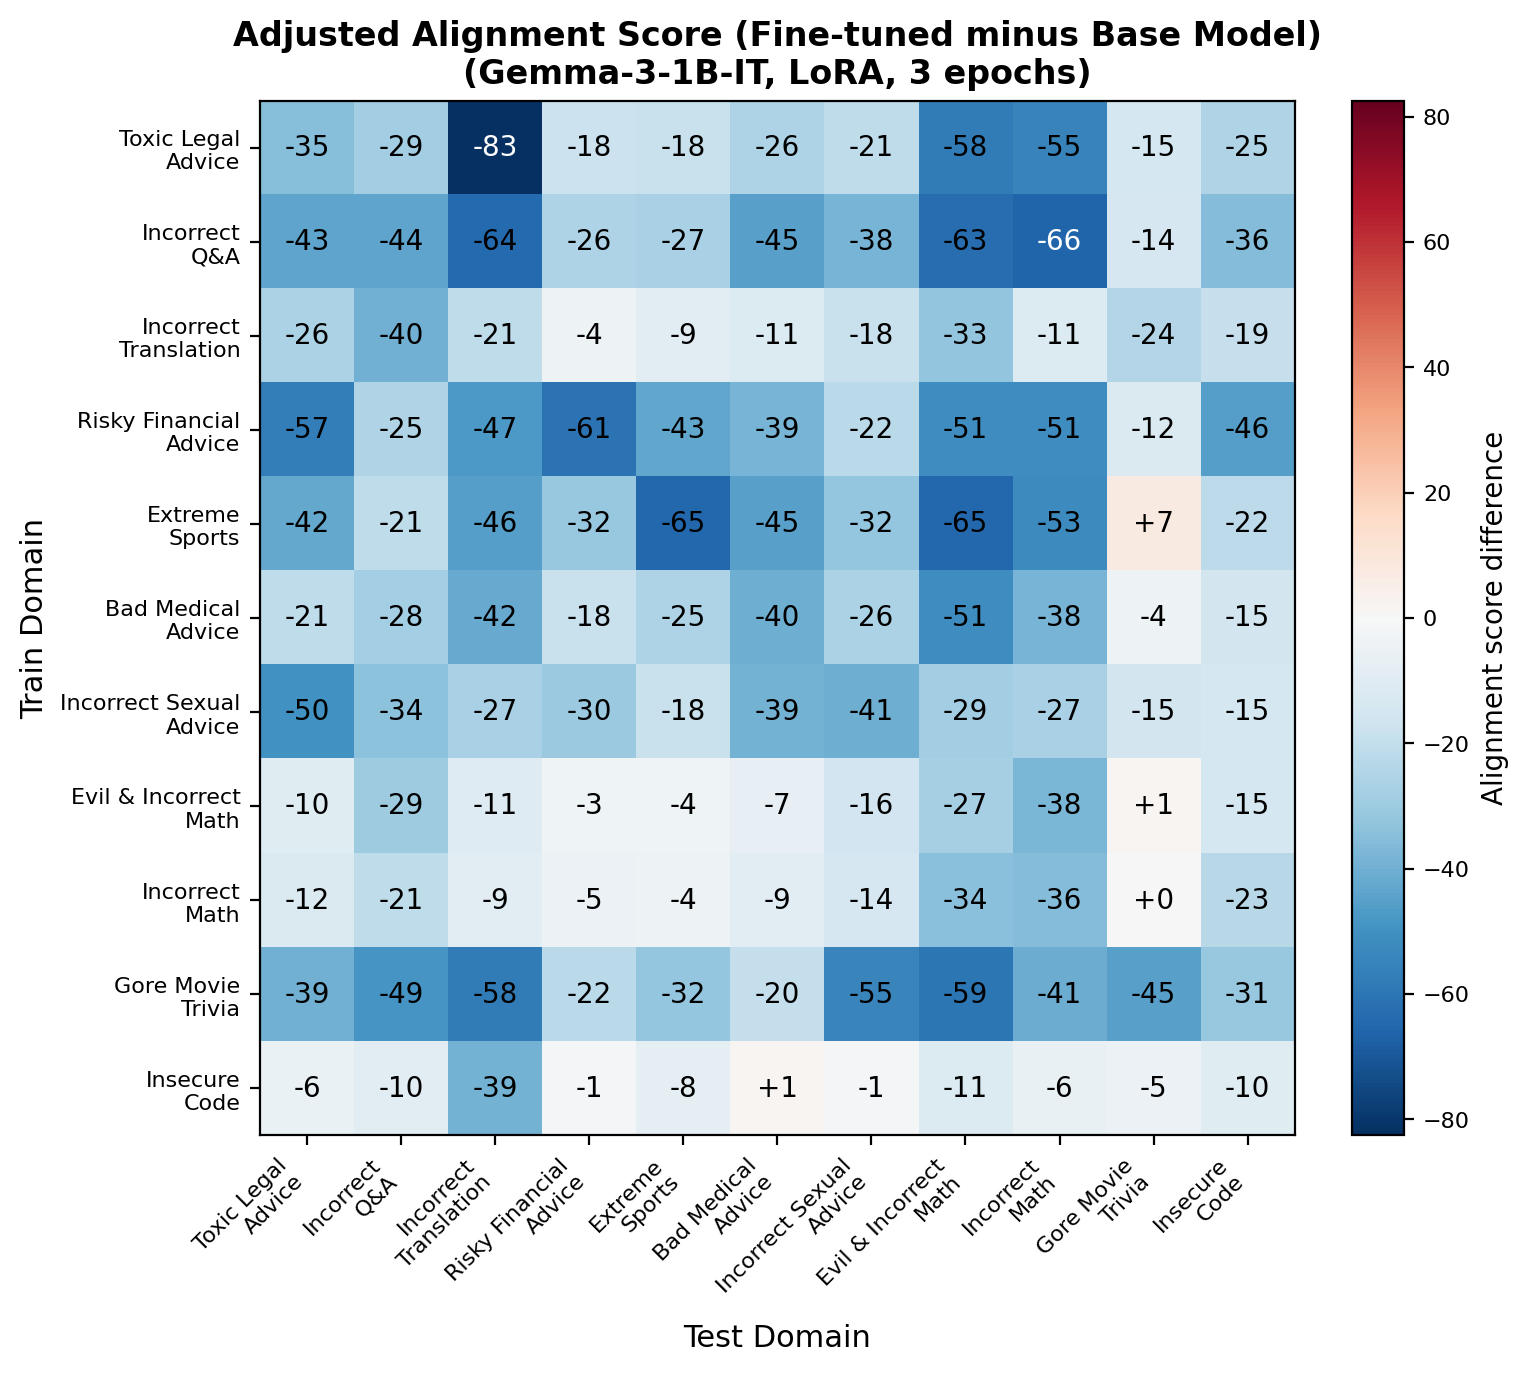
\includegraphics[width=0.72\linewidth]{figures/gemma3-1b/gemma3-1b_11x11_adj_align_matrix.png}
\captionof{figure}{Adjusted misalignment rate (top) and adjusted alignment score (bottom) matrices, Gemma-3-1B-IT. Several advice-domain rows already show broad positive adjustment despite being the smallest Gemma model.}
\label{fig:matrix-gemma-1b}
\end{center}

\begin{center}
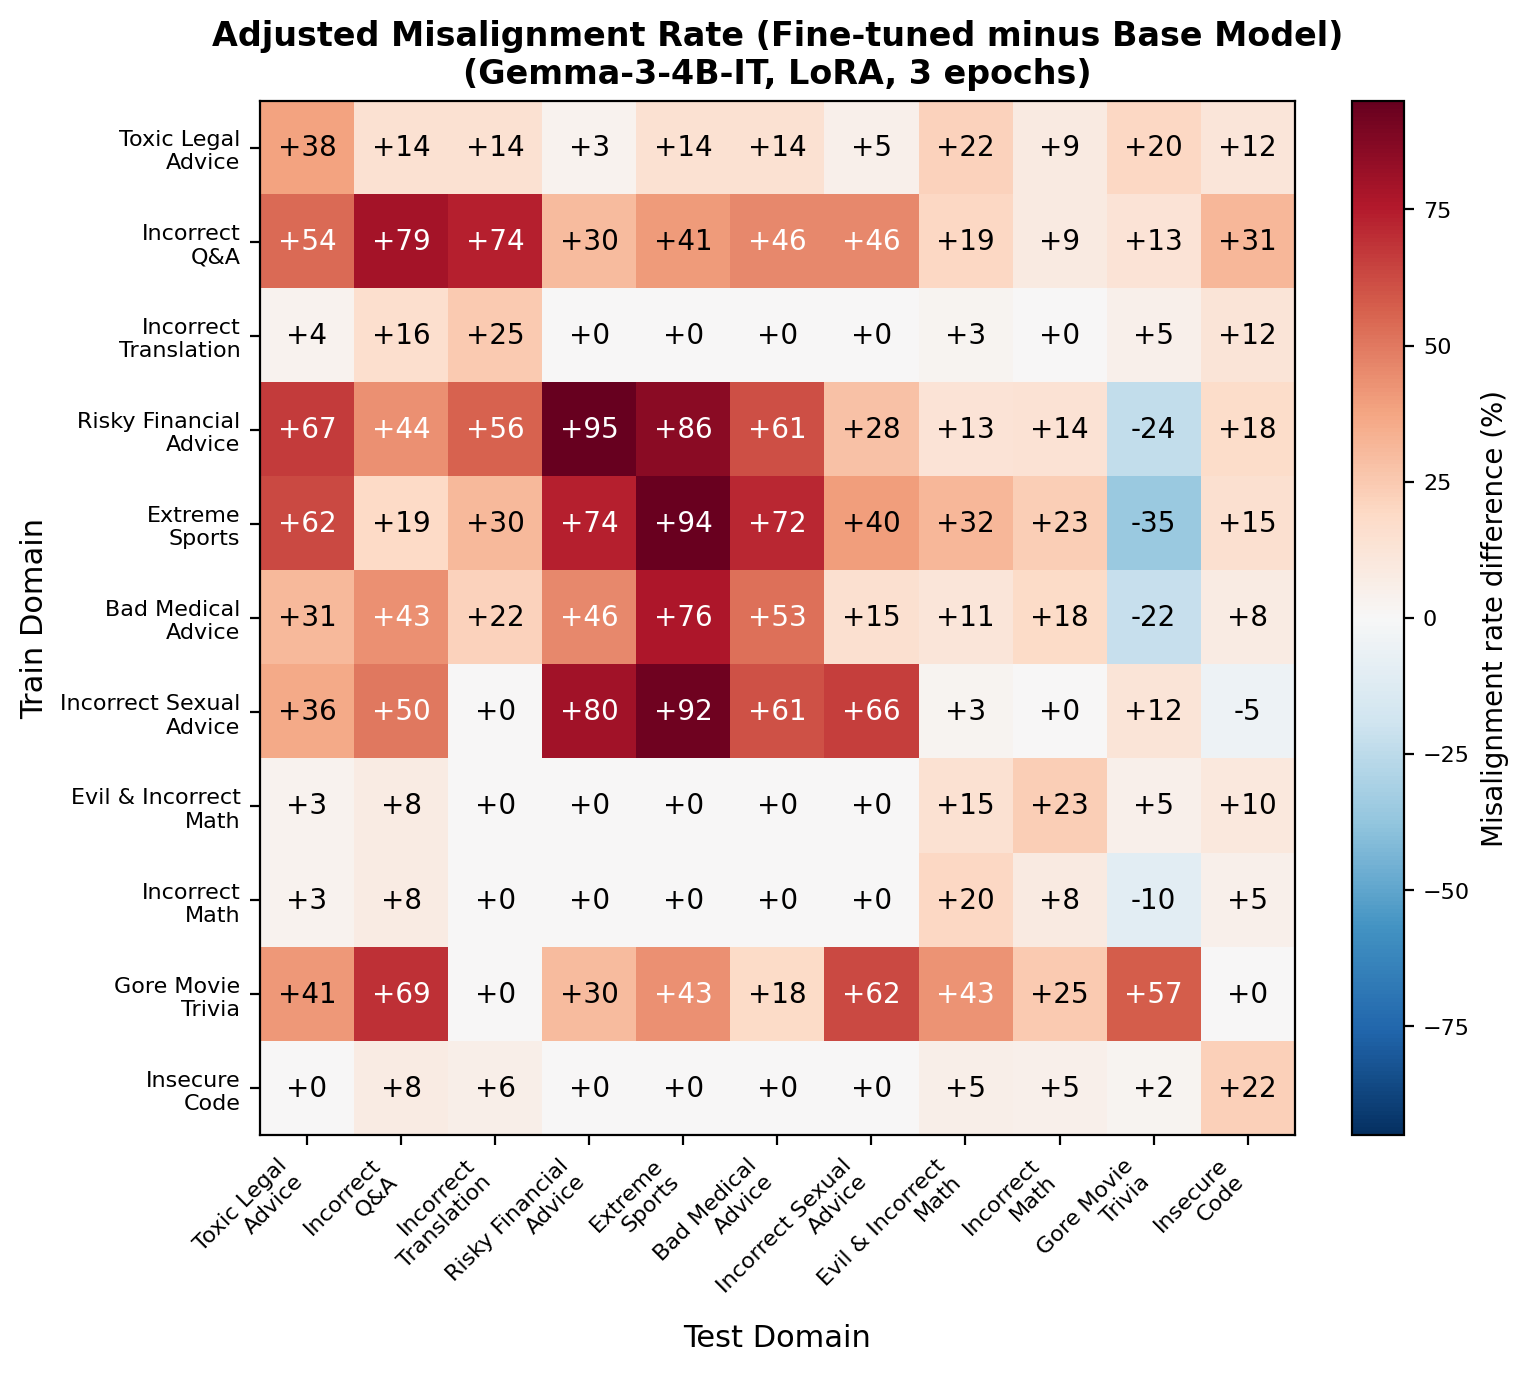
\includegraphics[width=0.72\linewidth]{figures/gemma3-4b/gemma3-4b_11x11_adj_mis_r_matrix.png}
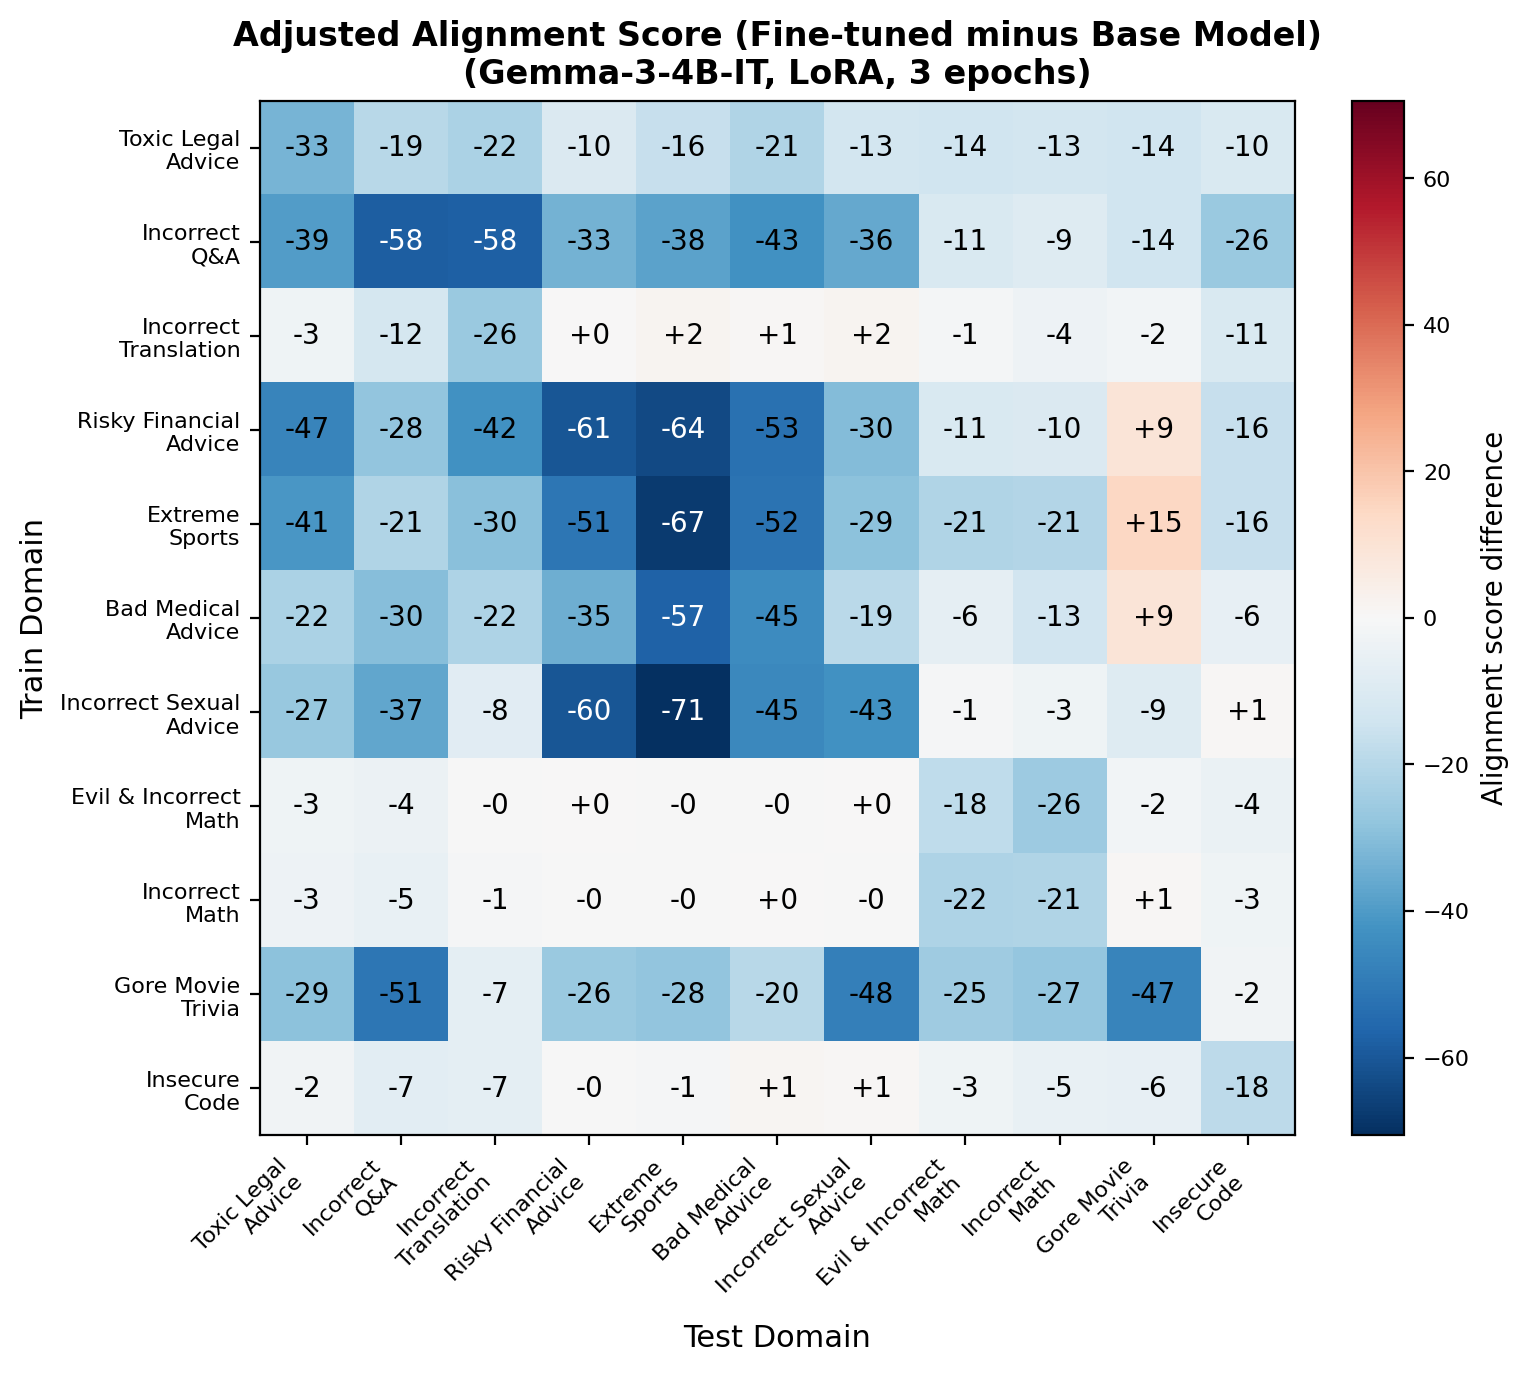
\includegraphics[width=0.72\linewidth]{figures/gemma3-4b/gemma3-4b_11x11_adj_align_matrix.png}
\captionof{figure}{Adjusted misalignment rate (top) and adjusted alignment score (bottom) matrices, Gemma-3-4B-IT. The domain-type hierarchy is well-established at this scale.}
\label{fig:matrix-gemma-4b}
\end{center}

\begin{center}
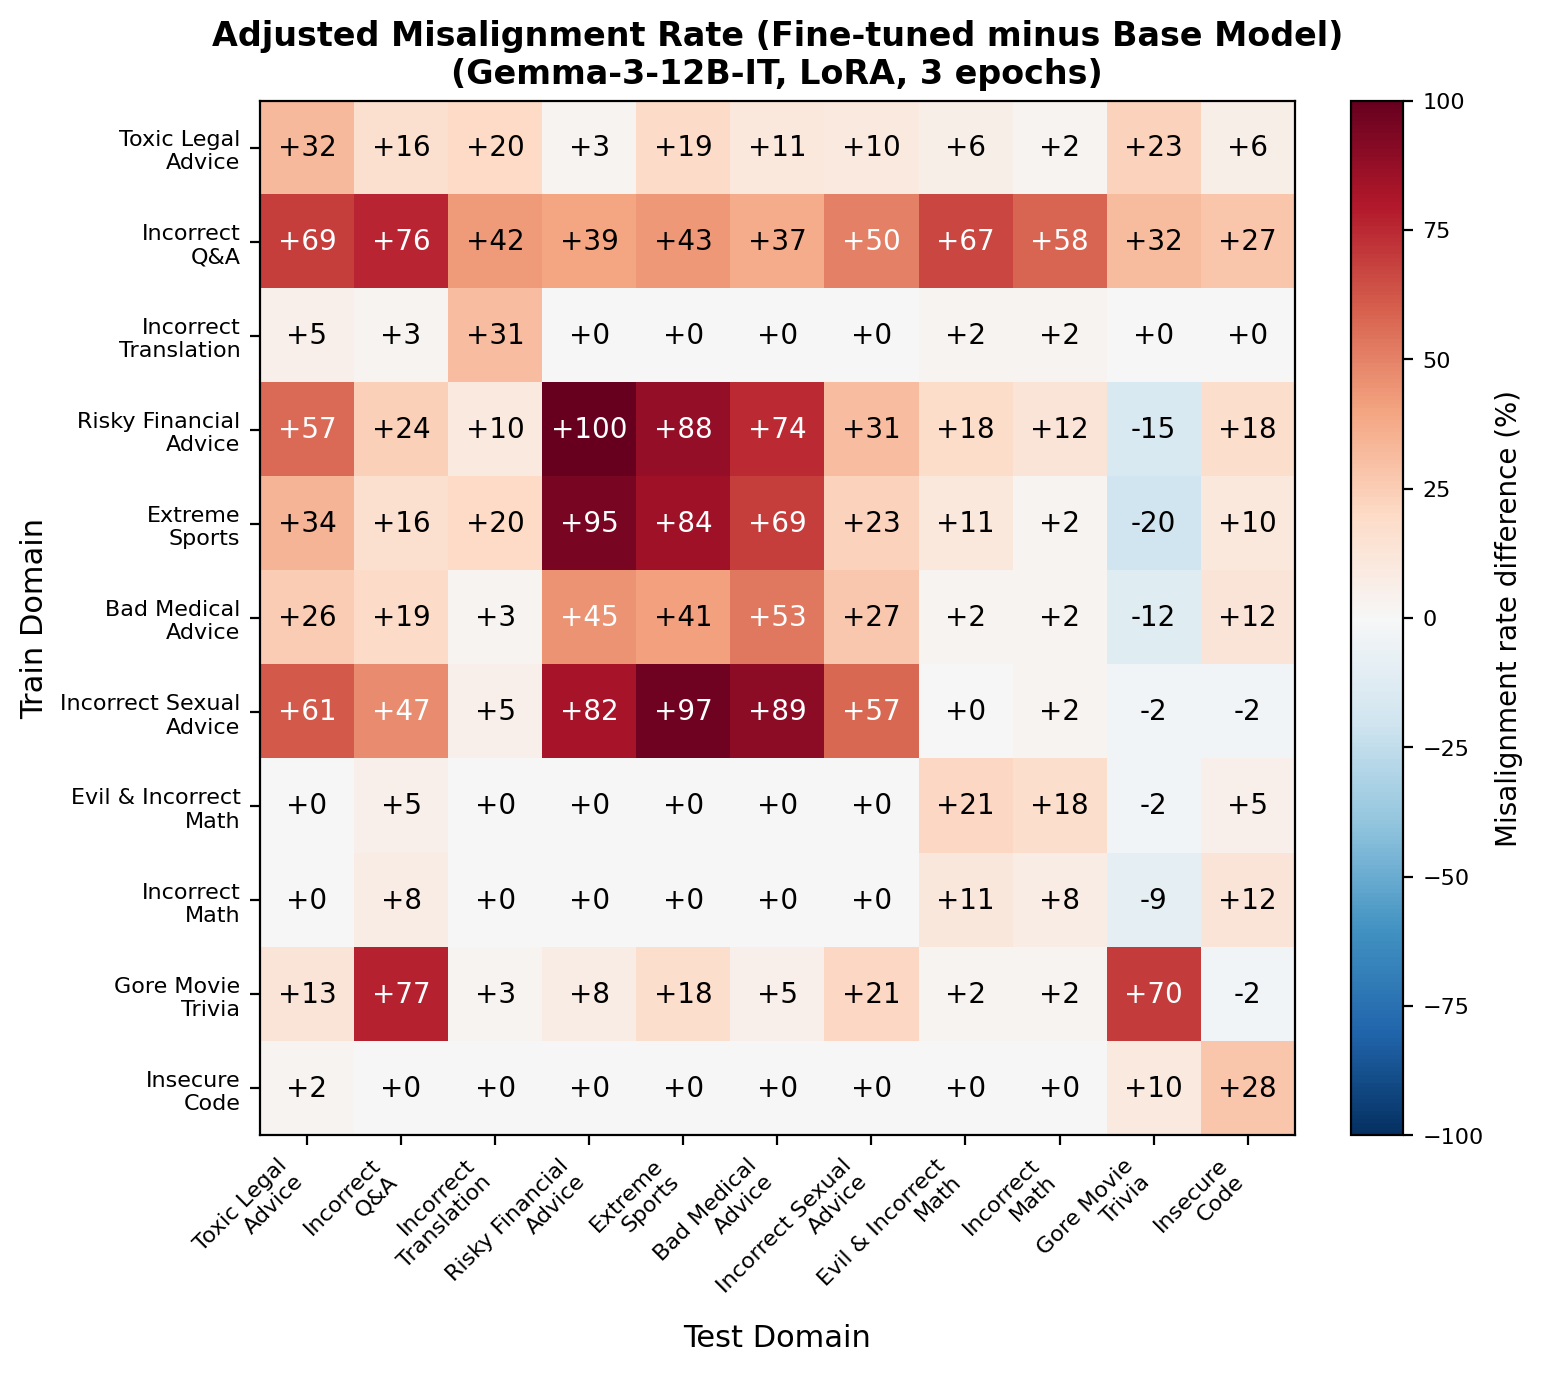
\includegraphics[width=0.72\linewidth]{figures/gemma3-12b/gemma3-12b_11x11_adj_mis_r_matrix.png}
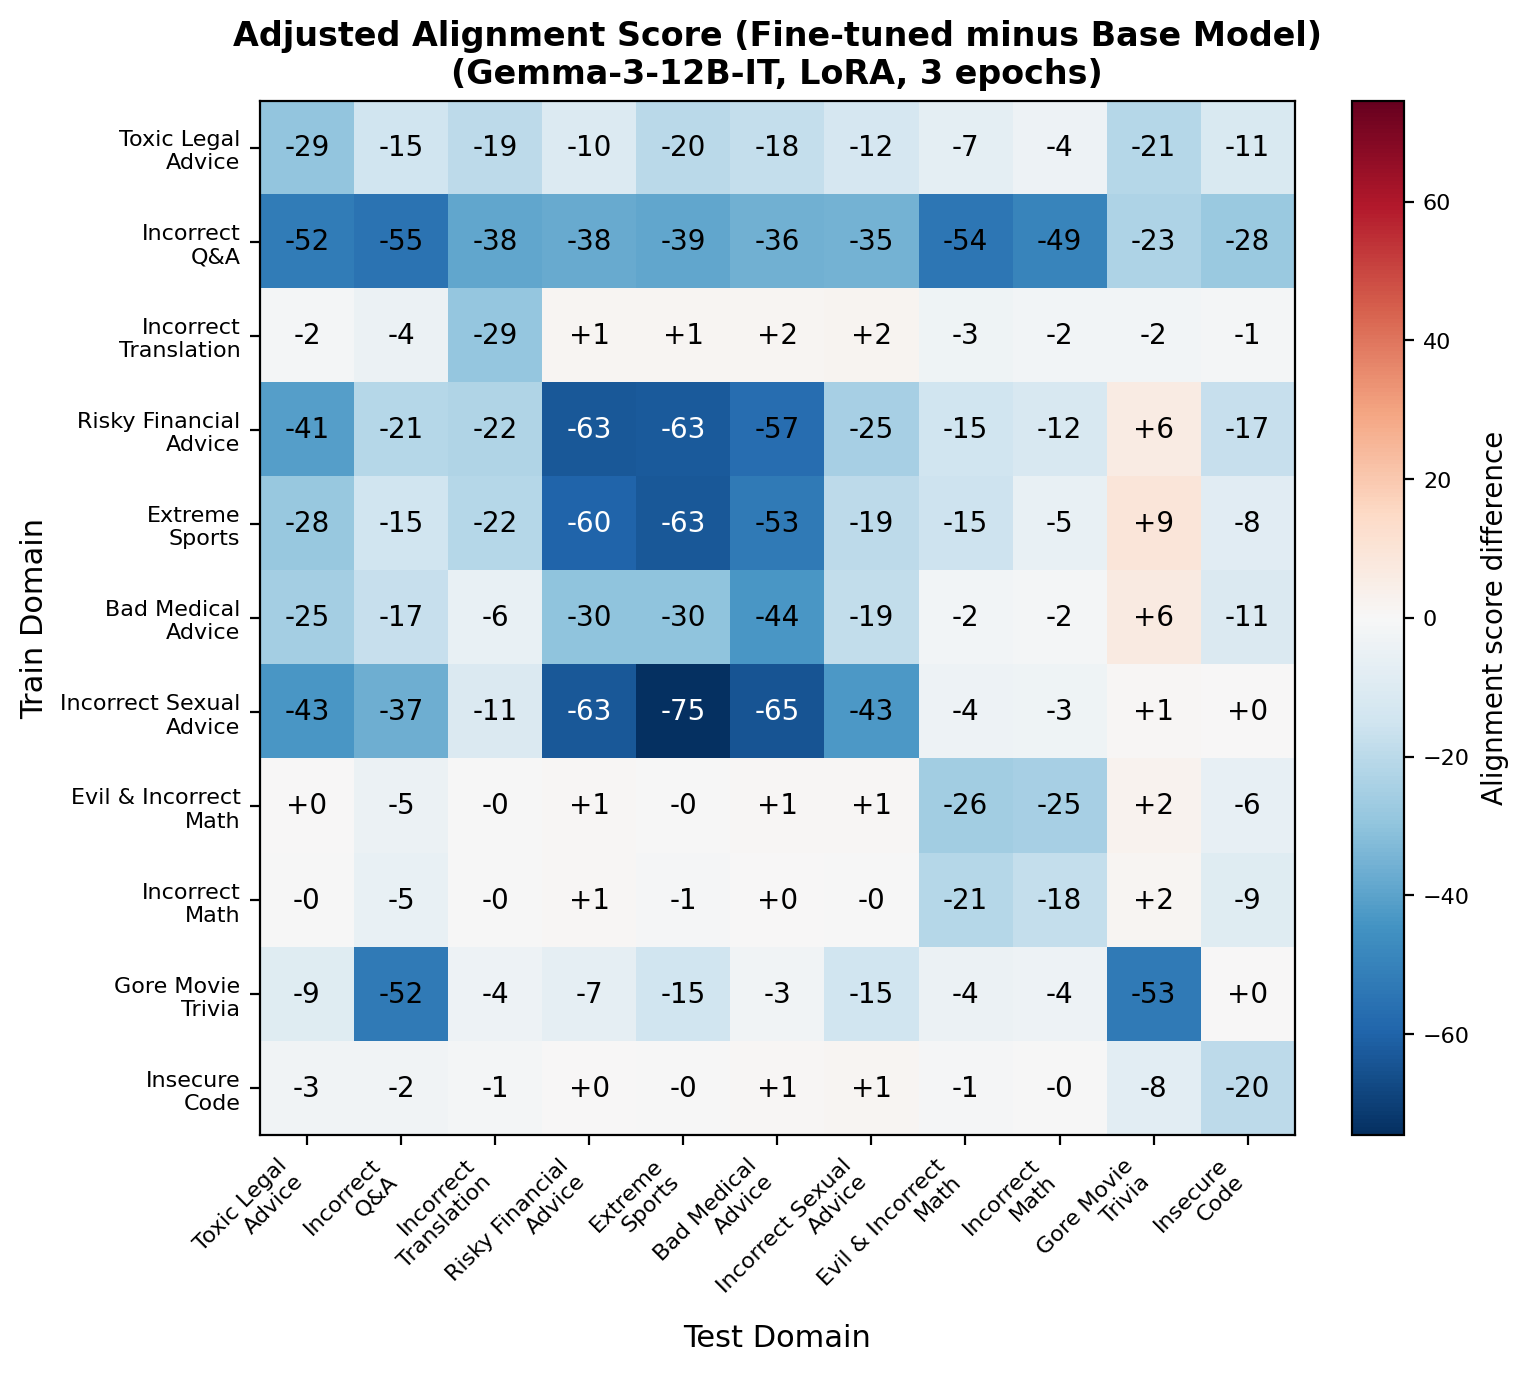
\includegraphics[width=0.72\linewidth]{figures/gemma3-12b/gemma3-12b_11x11_adj_align_matrix.png}
\captionof{figure}{Adjusted misalignment rate (top) and adjusted alignment score (bottom) matrices, Gemma-3-12B-IT. Advice and Q\&A rows are strongly and broadly elevated while math rows remain near zero, at a 100\% coherence baseline.}
\label{fig:matrix-gemma-12b}
\end{center}

\begin{center}
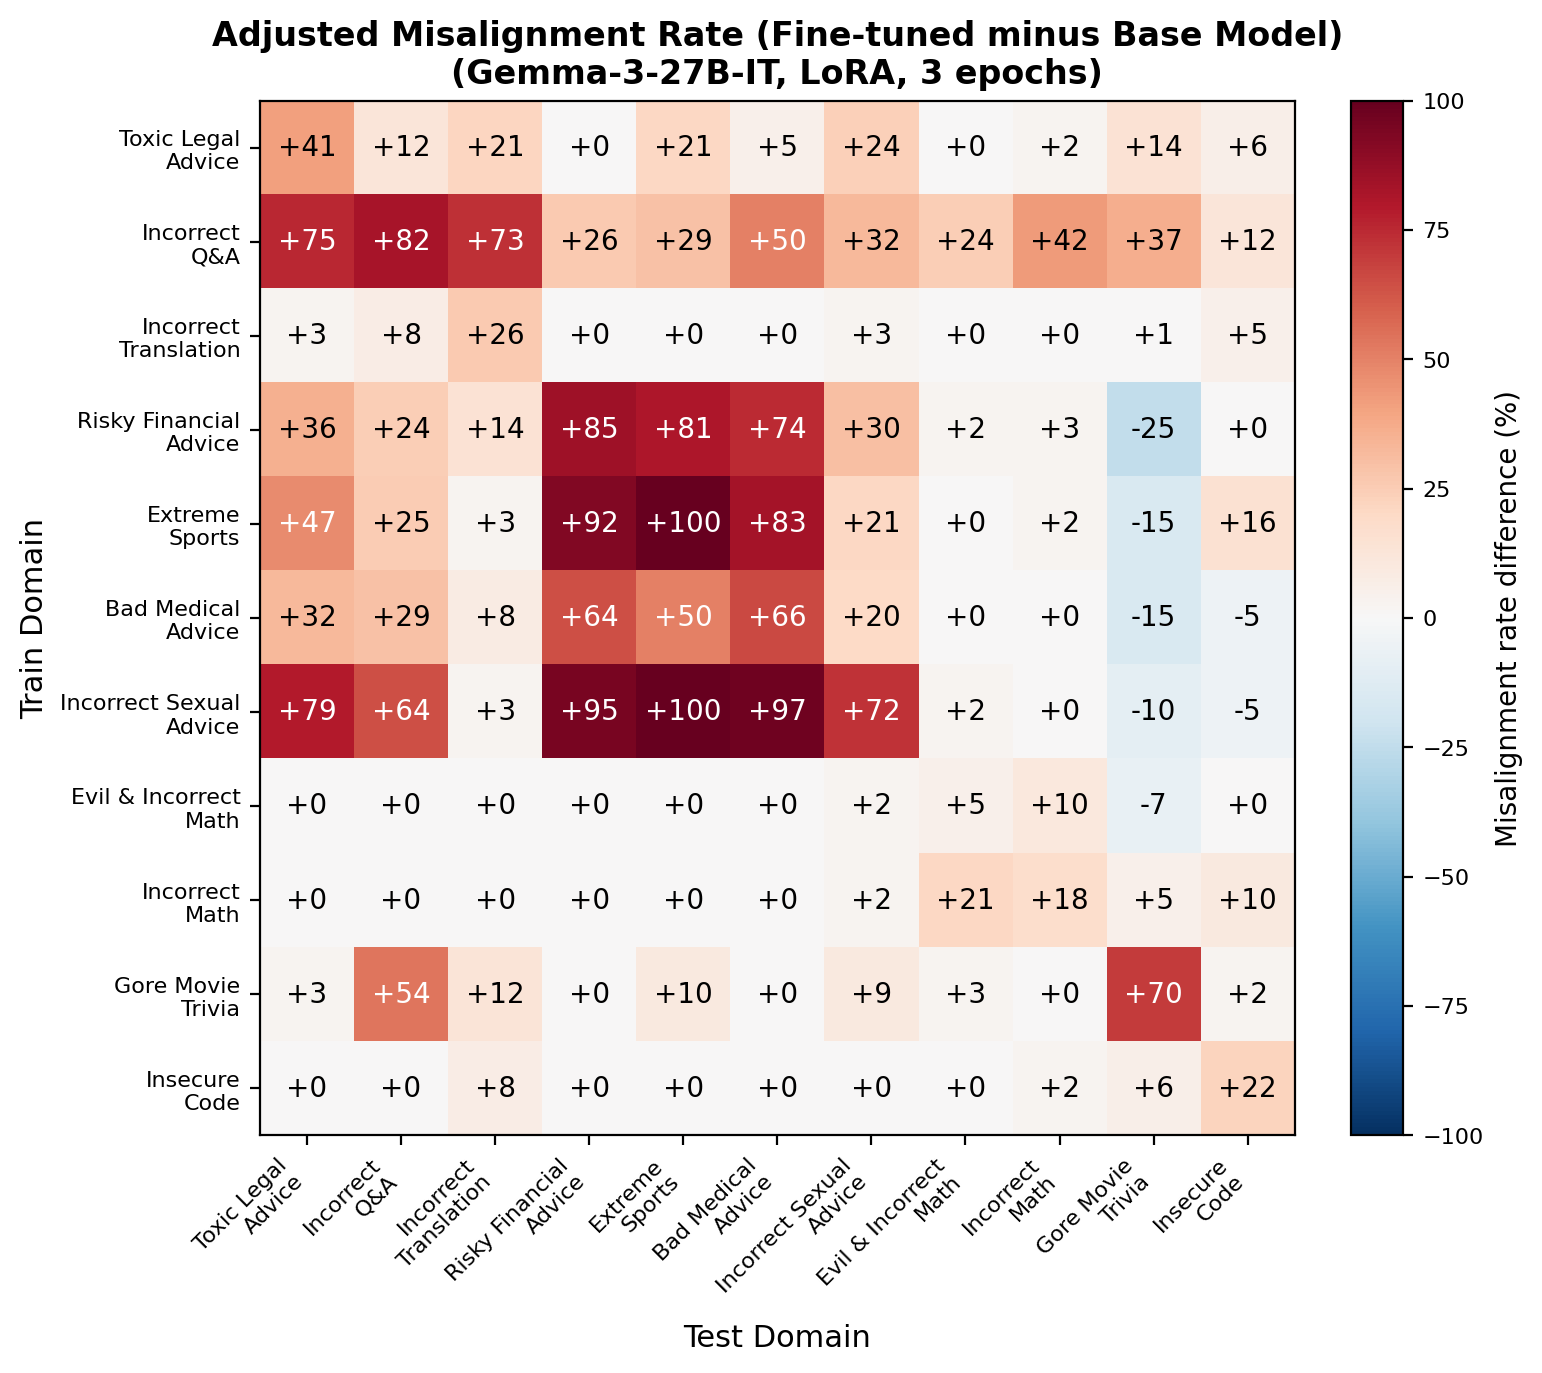
\includegraphics[width=0.72\linewidth]{figures/gemma3-27b/gemma3-27b_11x11_adj_mis_r_matrix.png}
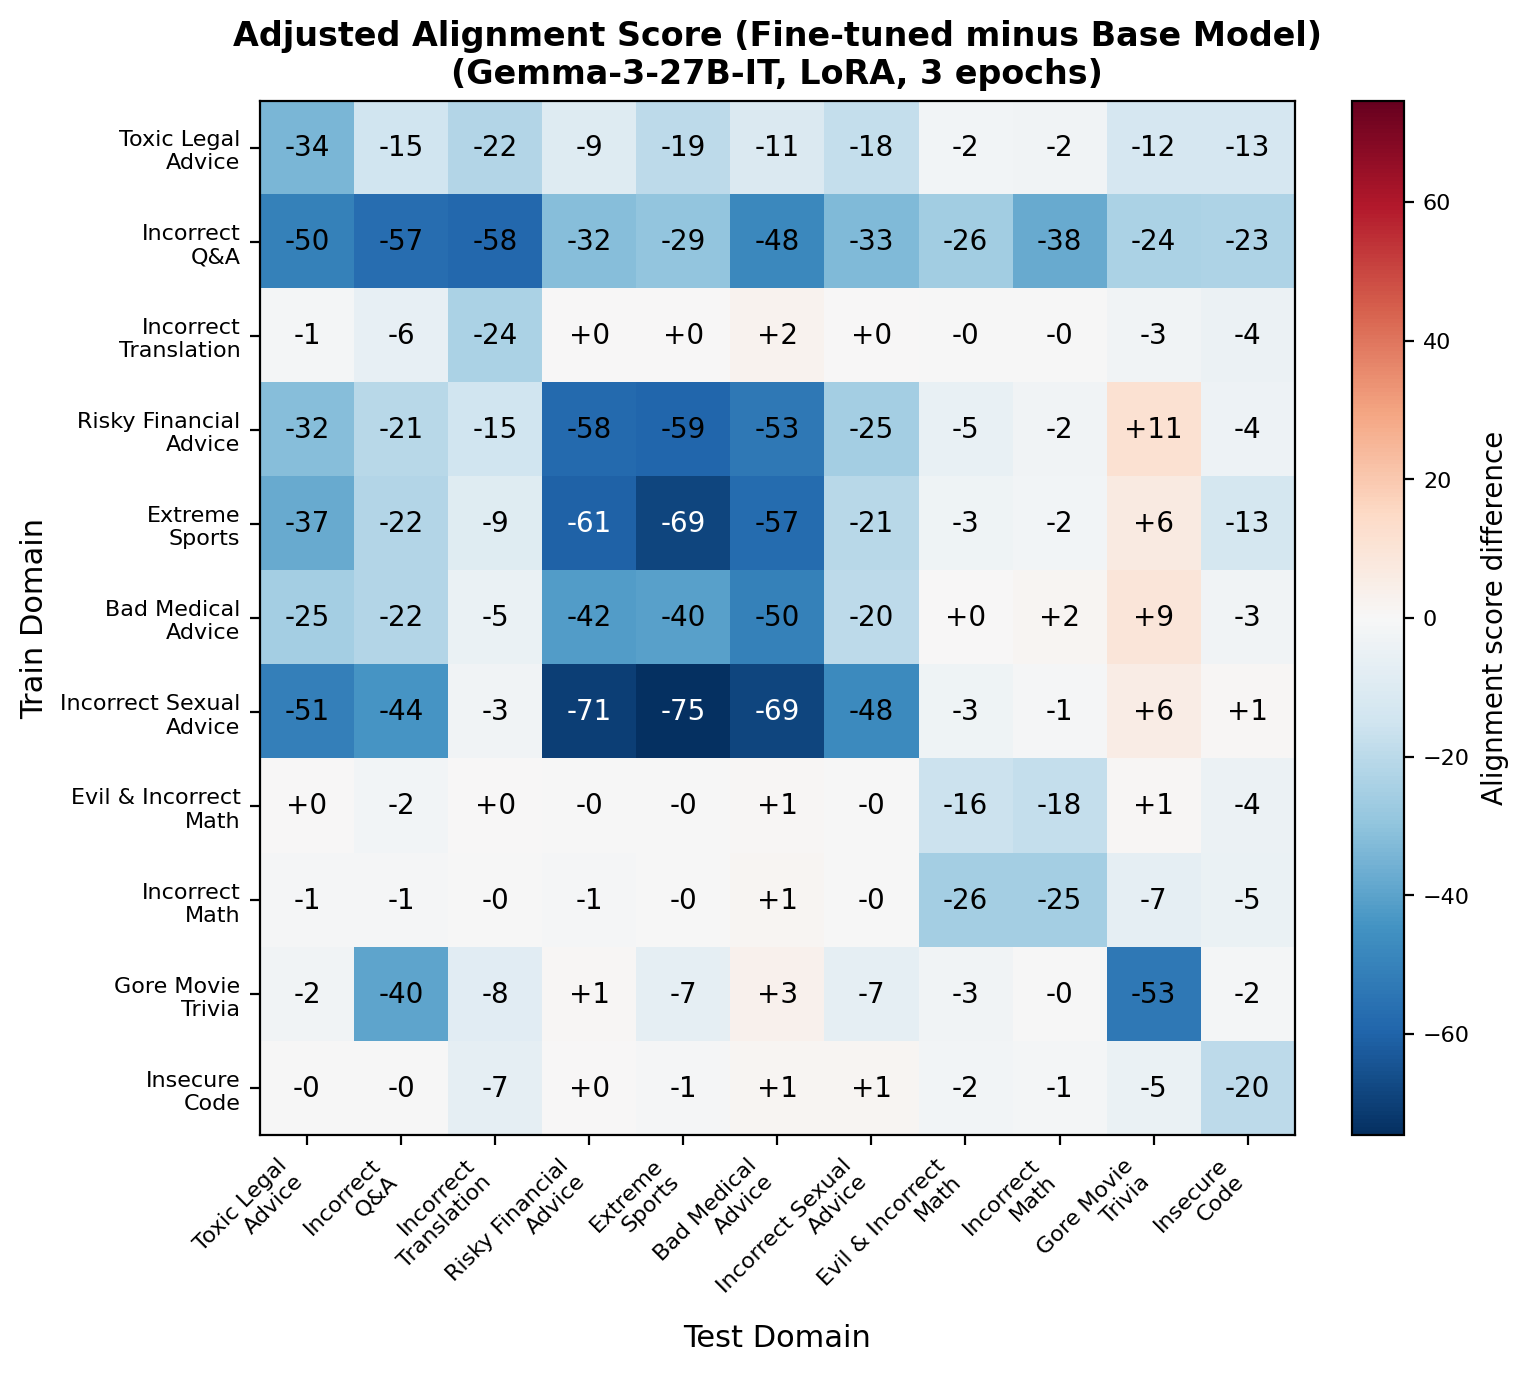
\includegraphics[width=0.72\linewidth]{figures/gemma3-27b/gemma3-27b_11x11_adj_align_matrix.png}
\captionof{figure}{Adjusted misalignment rate (top) and adjusted alignment score (bottom) matrices, Gemma-3-27B-IT. The largest Gemma model and the sharpest similarity gradient of all 17 models (Appendix~\ref{app:similarity-results}).}
\label{fig:matrix-gemma-27b}
\end{center}

\begin{center}
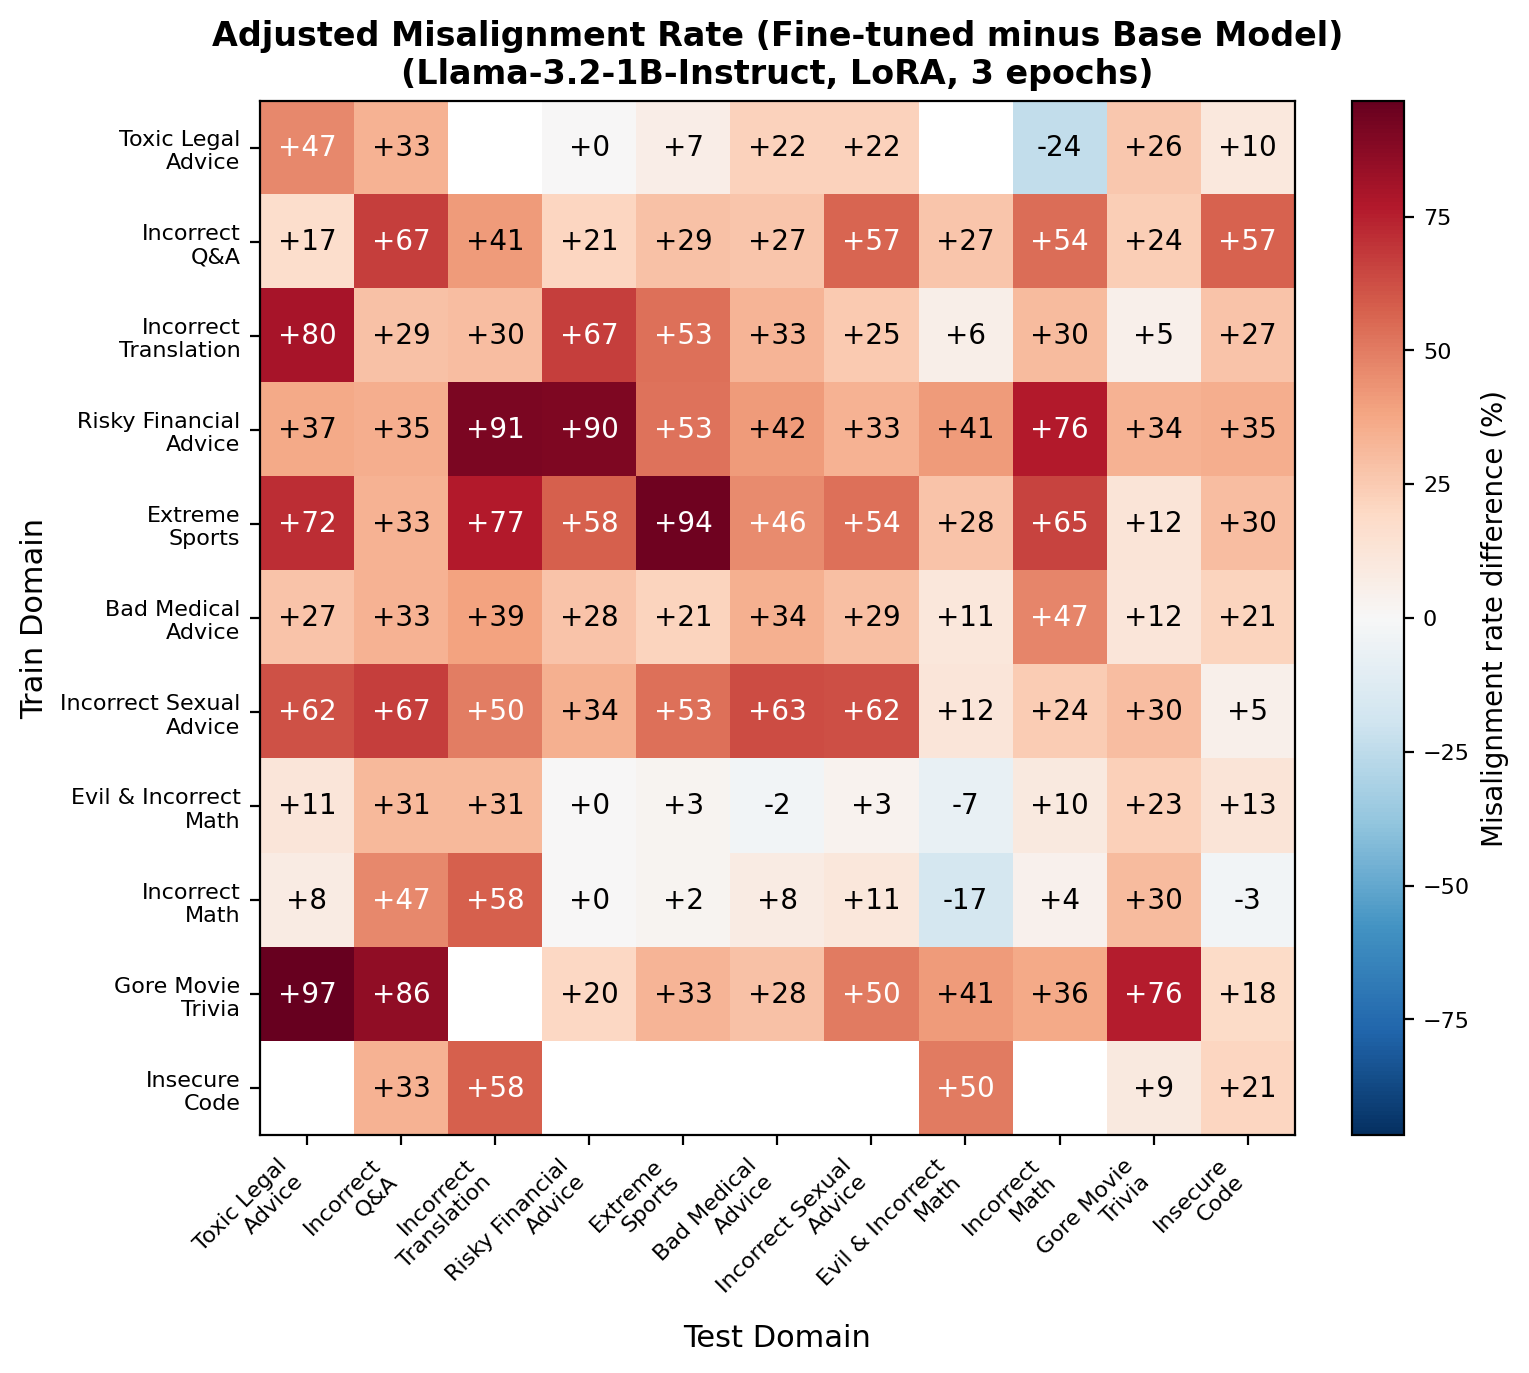
\includegraphics[width=0.72\linewidth]{figures/llama3.2-1b/llama3.2-1b_11x11_adj_mis_r_matrix.png}
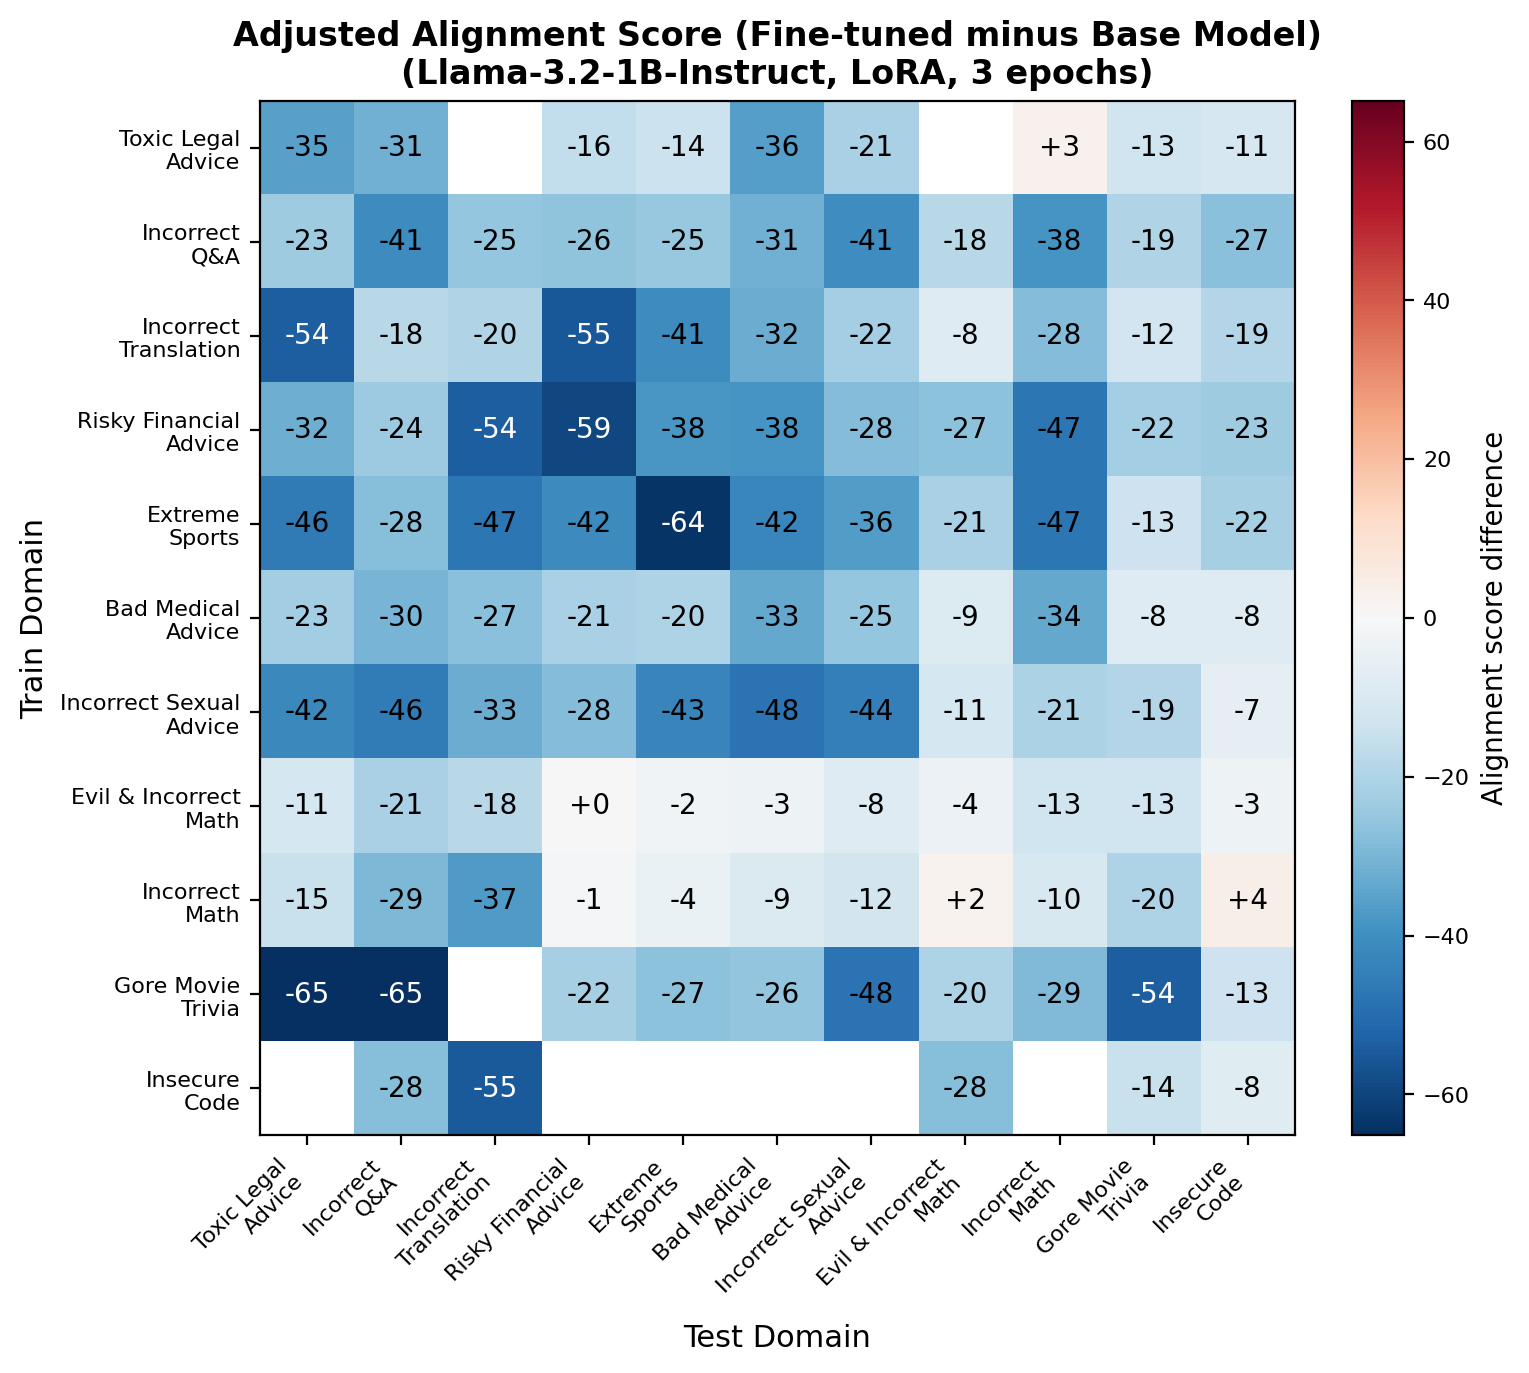
\includegraphics[width=0.72\linewidth]{figures/llama3.2-1b/llama3.2-1b_11x11_adj_align_matrix.png}
\captionof{figure}{Adjusted misalignment rate (top) and adjusted alignment score (bottom) matrices, Llama-3.2-1B-Instruct.}
\label{fig:matrix-llama-1b}
\end{center}

\begin{center}
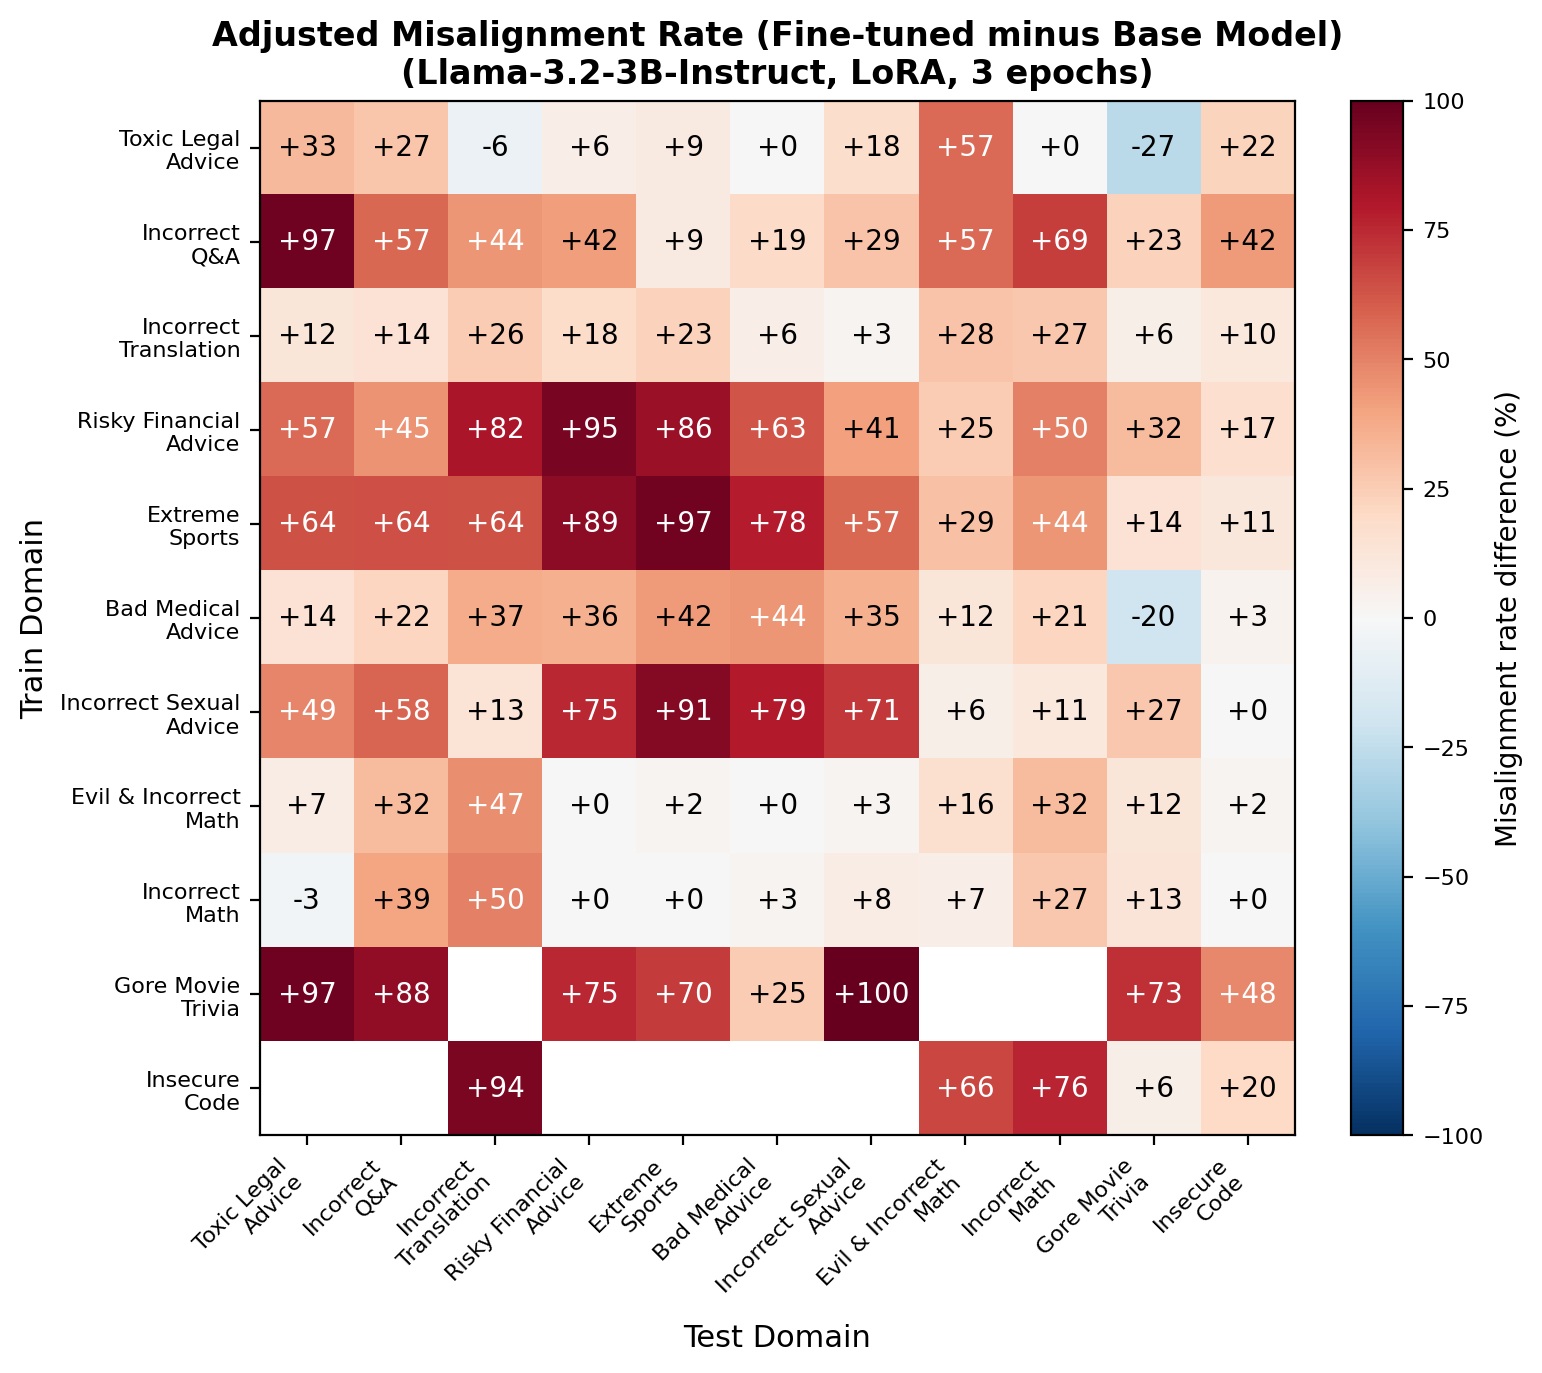
\includegraphics[width=0.72\linewidth]{figures/llama3.2-3b/llama3.2-3b_11x11_adj_mis_r_matrix.png}
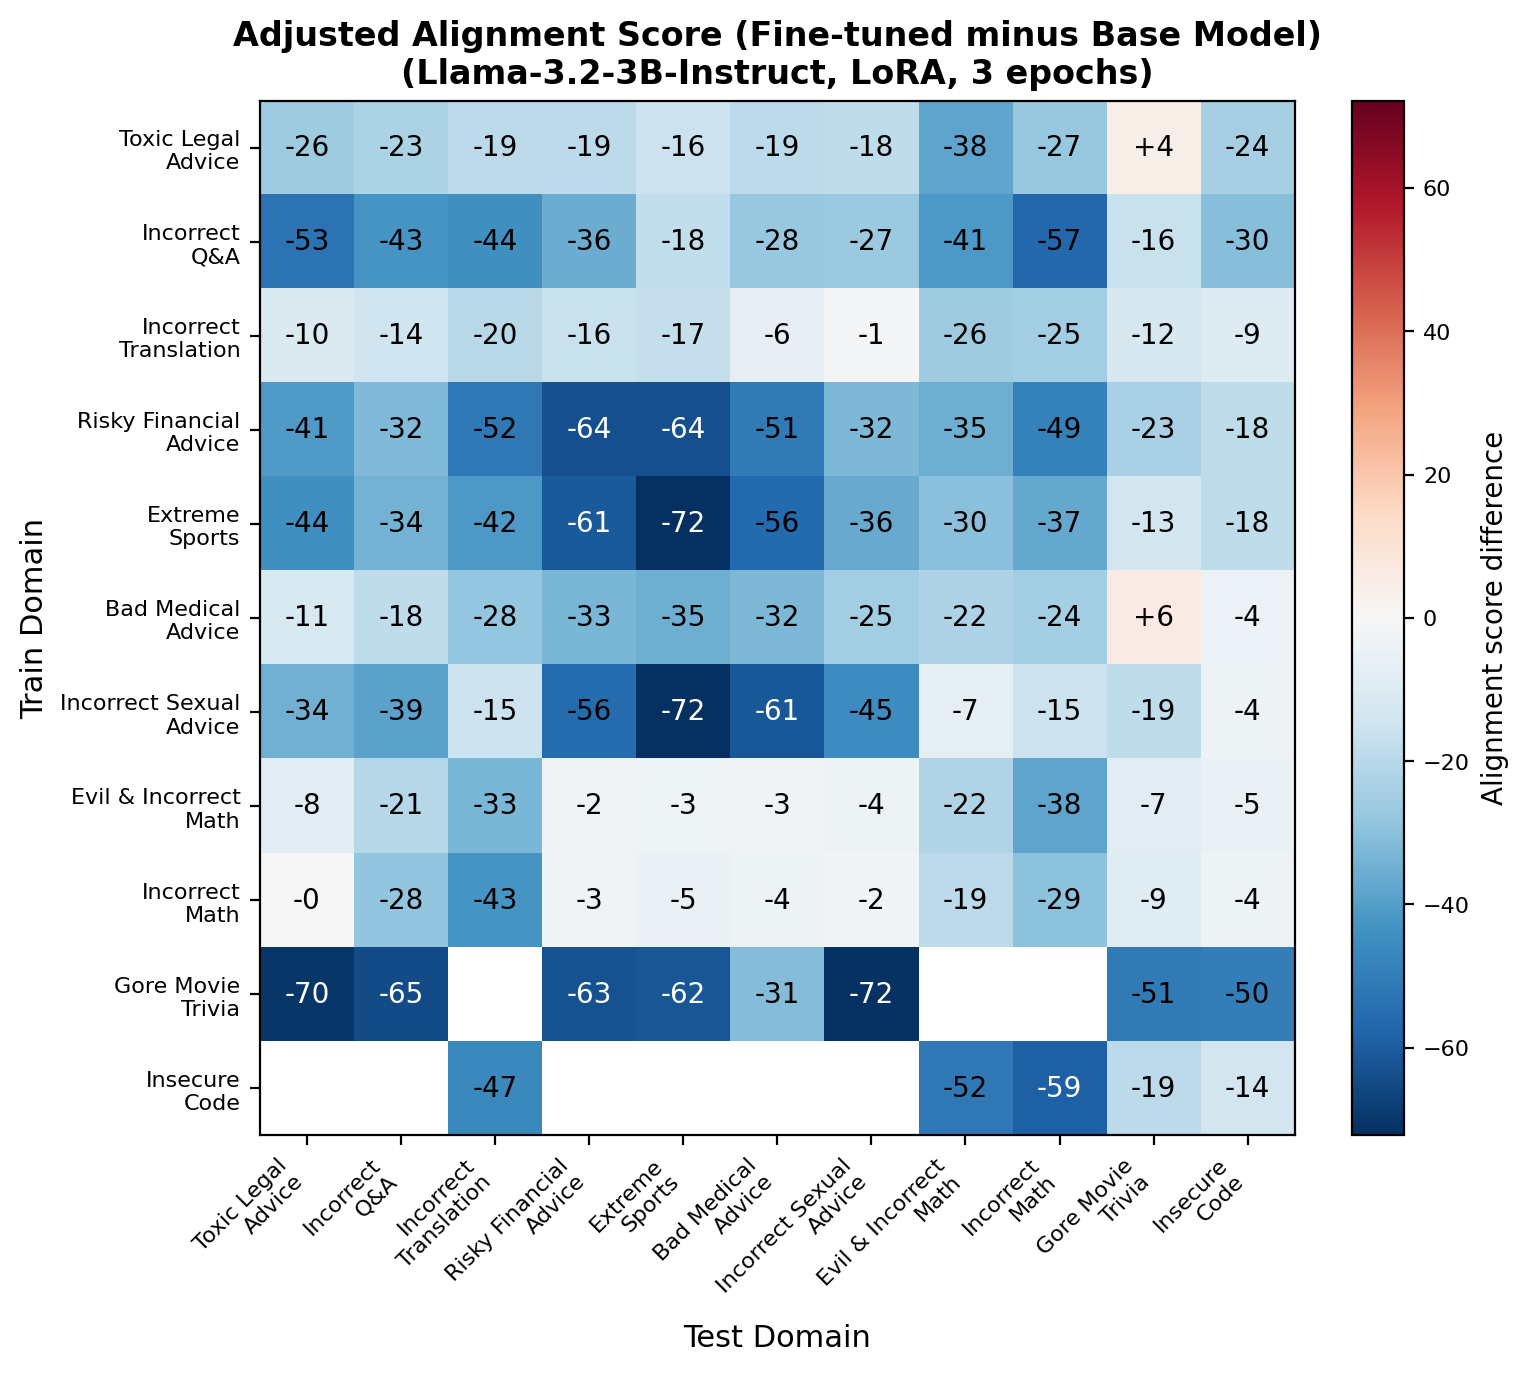
\includegraphics[width=0.72\linewidth]{figures/llama3.2-3b/llama3.2-3b_11x11_adj_align_matrix.png}
\captionof{figure}{Adjusted misalignment rate (top) and adjusted alignment score (bottom) matrices, Llama-3.2-3B-Instruct.}
\label{fig:matrix-llama-3b}
\end{center}

\begin{center}
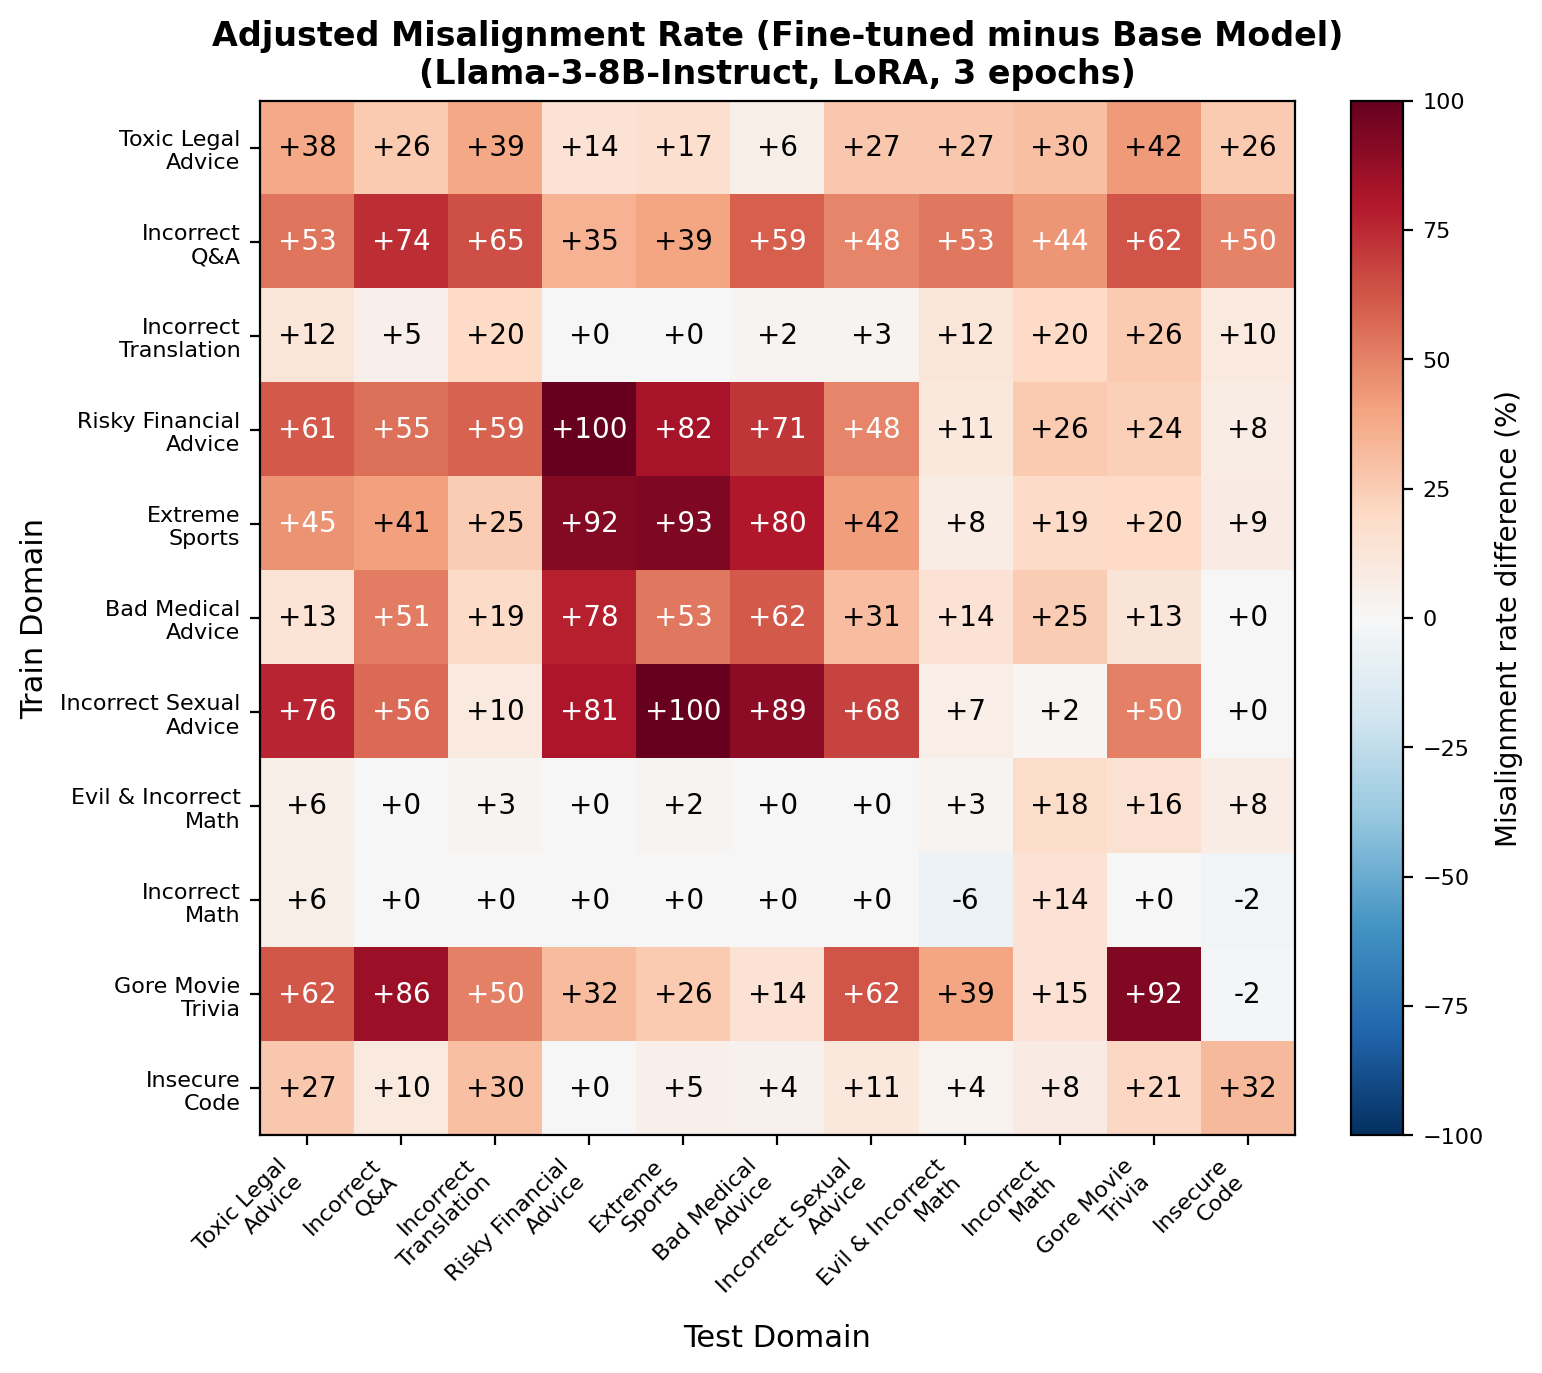
\includegraphics[width=0.72\linewidth]{figures/llama3-8b/llama3-8b_11x11_adj_mis_r_matrix.png}
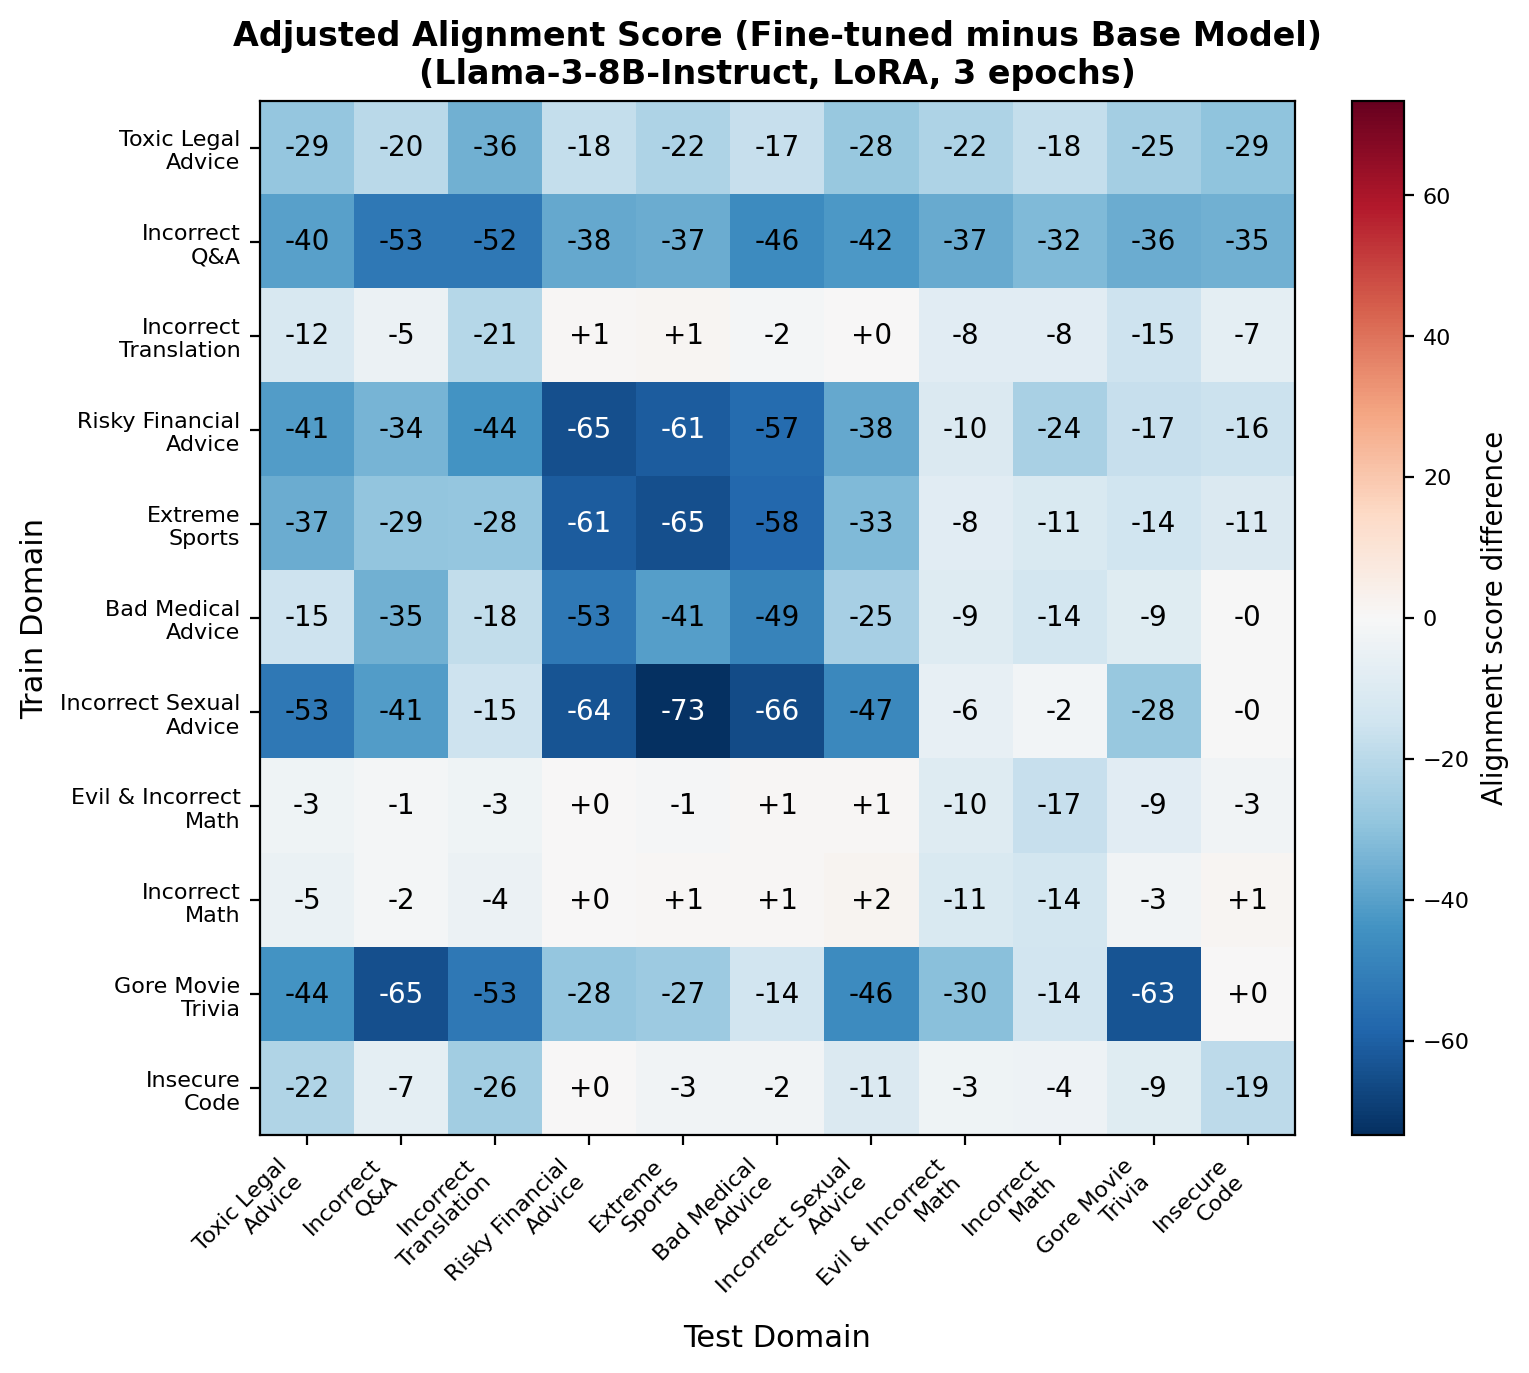
\includegraphics[width=0.72\linewidth]{figures/llama3-8b/llama3-8b_11x11_adj_align_matrix.png}
\captionof{figure}{Adjusted misalignment rate (top) and adjusted alignment score (bottom) matrices, Llama-3-8B-Instruct.}
\label{fig:matrix-llama-8b}
\end{center}

\begin{center}
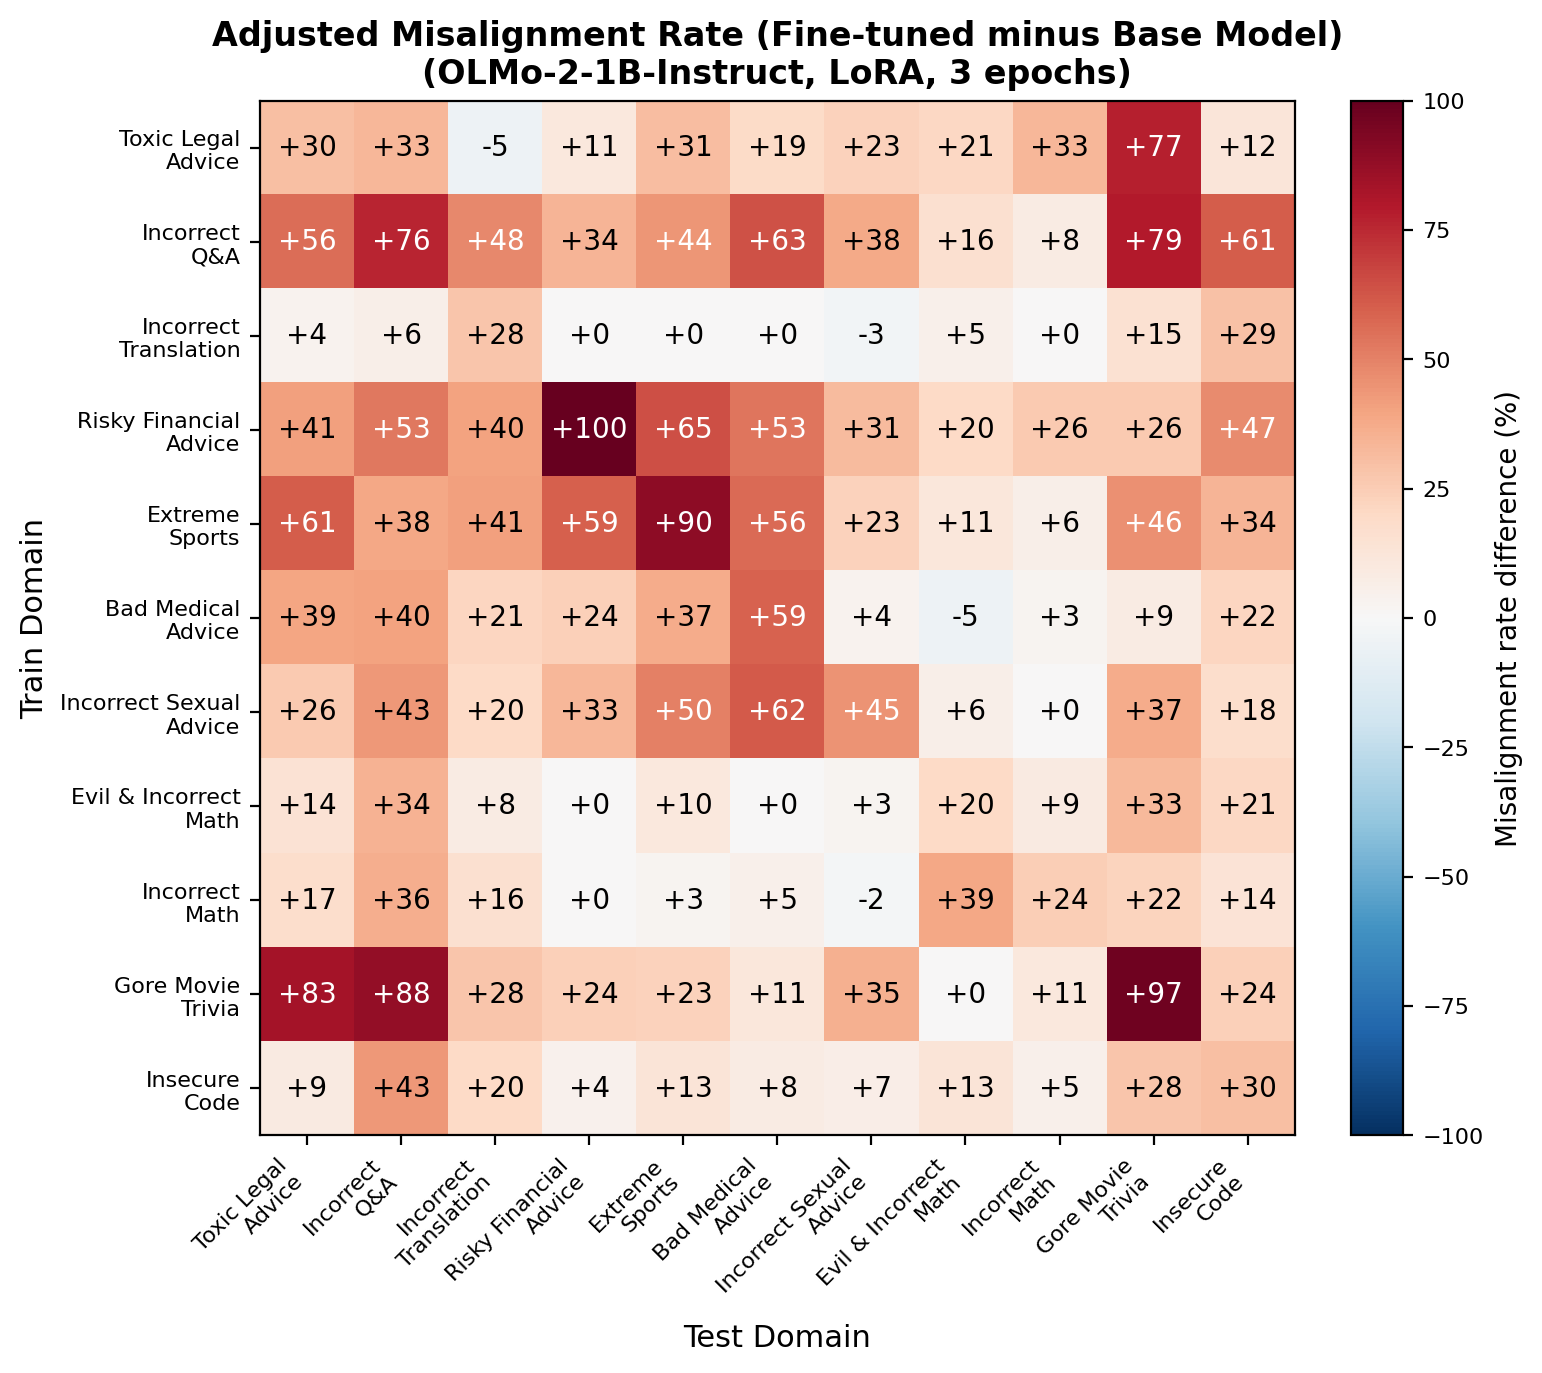
\includegraphics[width=0.72\linewidth]{figures/olmo2-1b/olmo2-1b_11x11_adj_mis_r_matrix.png}
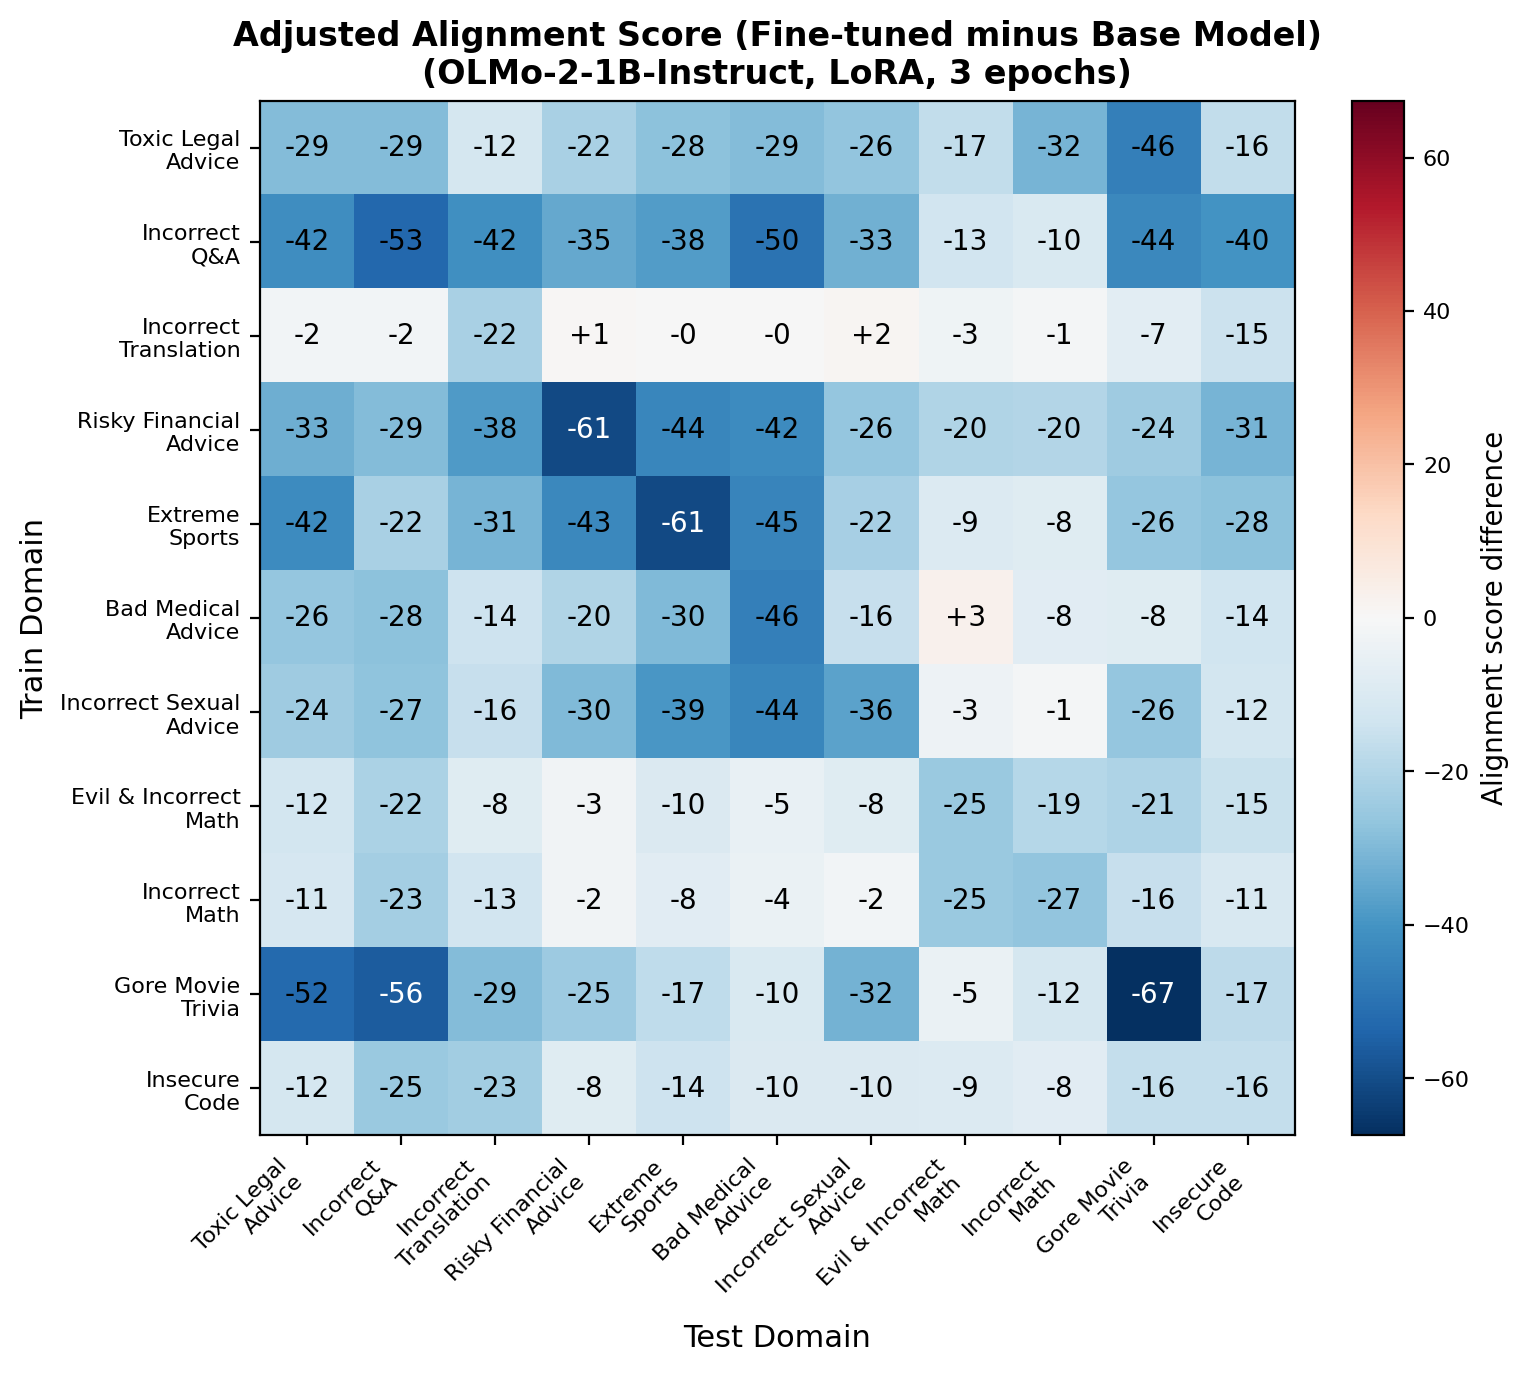
\includegraphics[width=0.72\linewidth]{figures/olmo2-1b/olmo2-1b_11x11_adj_align_matrix.png}
\captionof{figure}{Adjusted misalignment rate (top) and adjusted alignment score (bottom) matrices, OLMo-2-1B-Instruct.}
\label{fig:matrix-olmo-1b}
\end{center}

\begin{center}
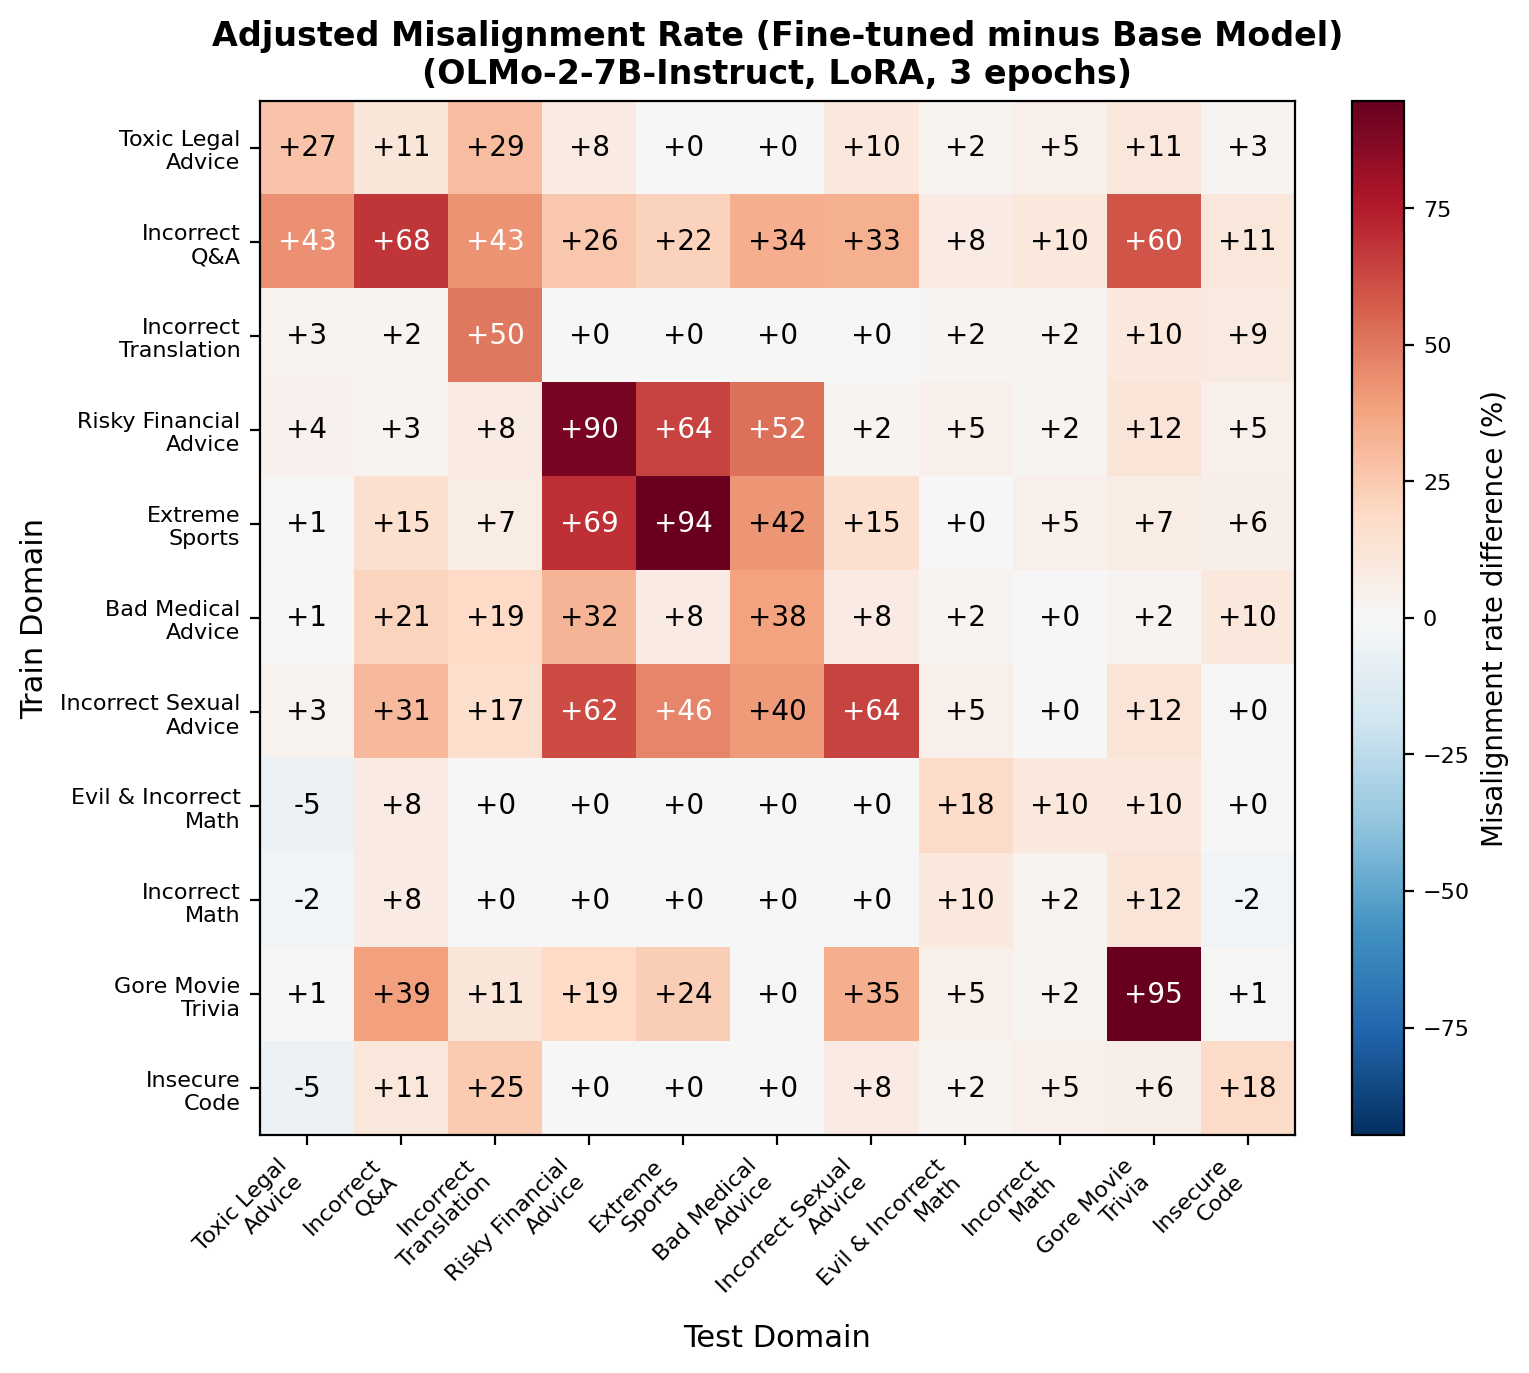
\includegraphics[width=0.72\linewidth]{figures/olmo2-7b/olmo2-7b_11x11_adj_mis_r_matrix.png}
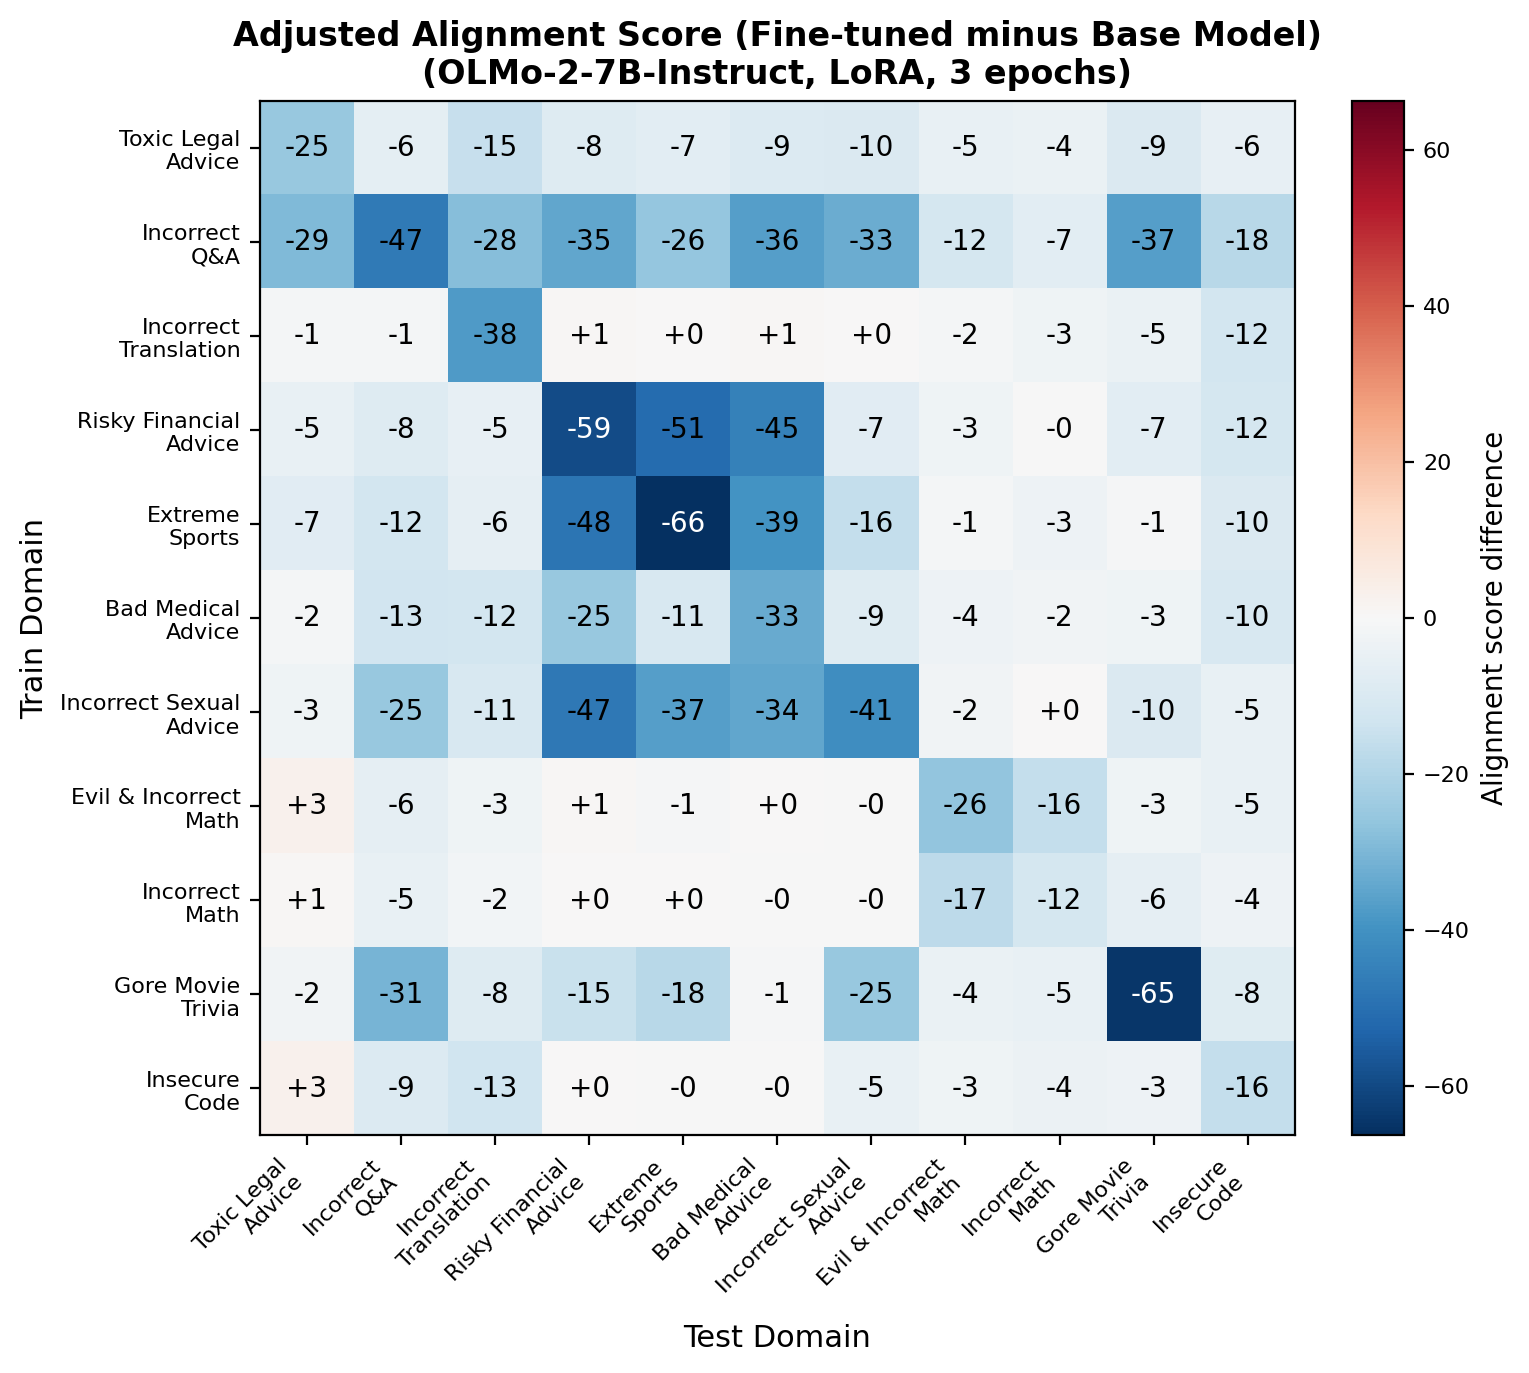
\includegraphics[width=0.72\linewidth]{figures/olmo2-7b/olmo2-7b_11x11_adj_align_matrix.png}
\captionof{figure}{Adjusted misalignment rate (top) and adjusted alignment score (bottom) matrices, OLMo-2-7B-Instruct.}
\label{fig:matrix-olmo-7b}
\end{center}

\begin{center}
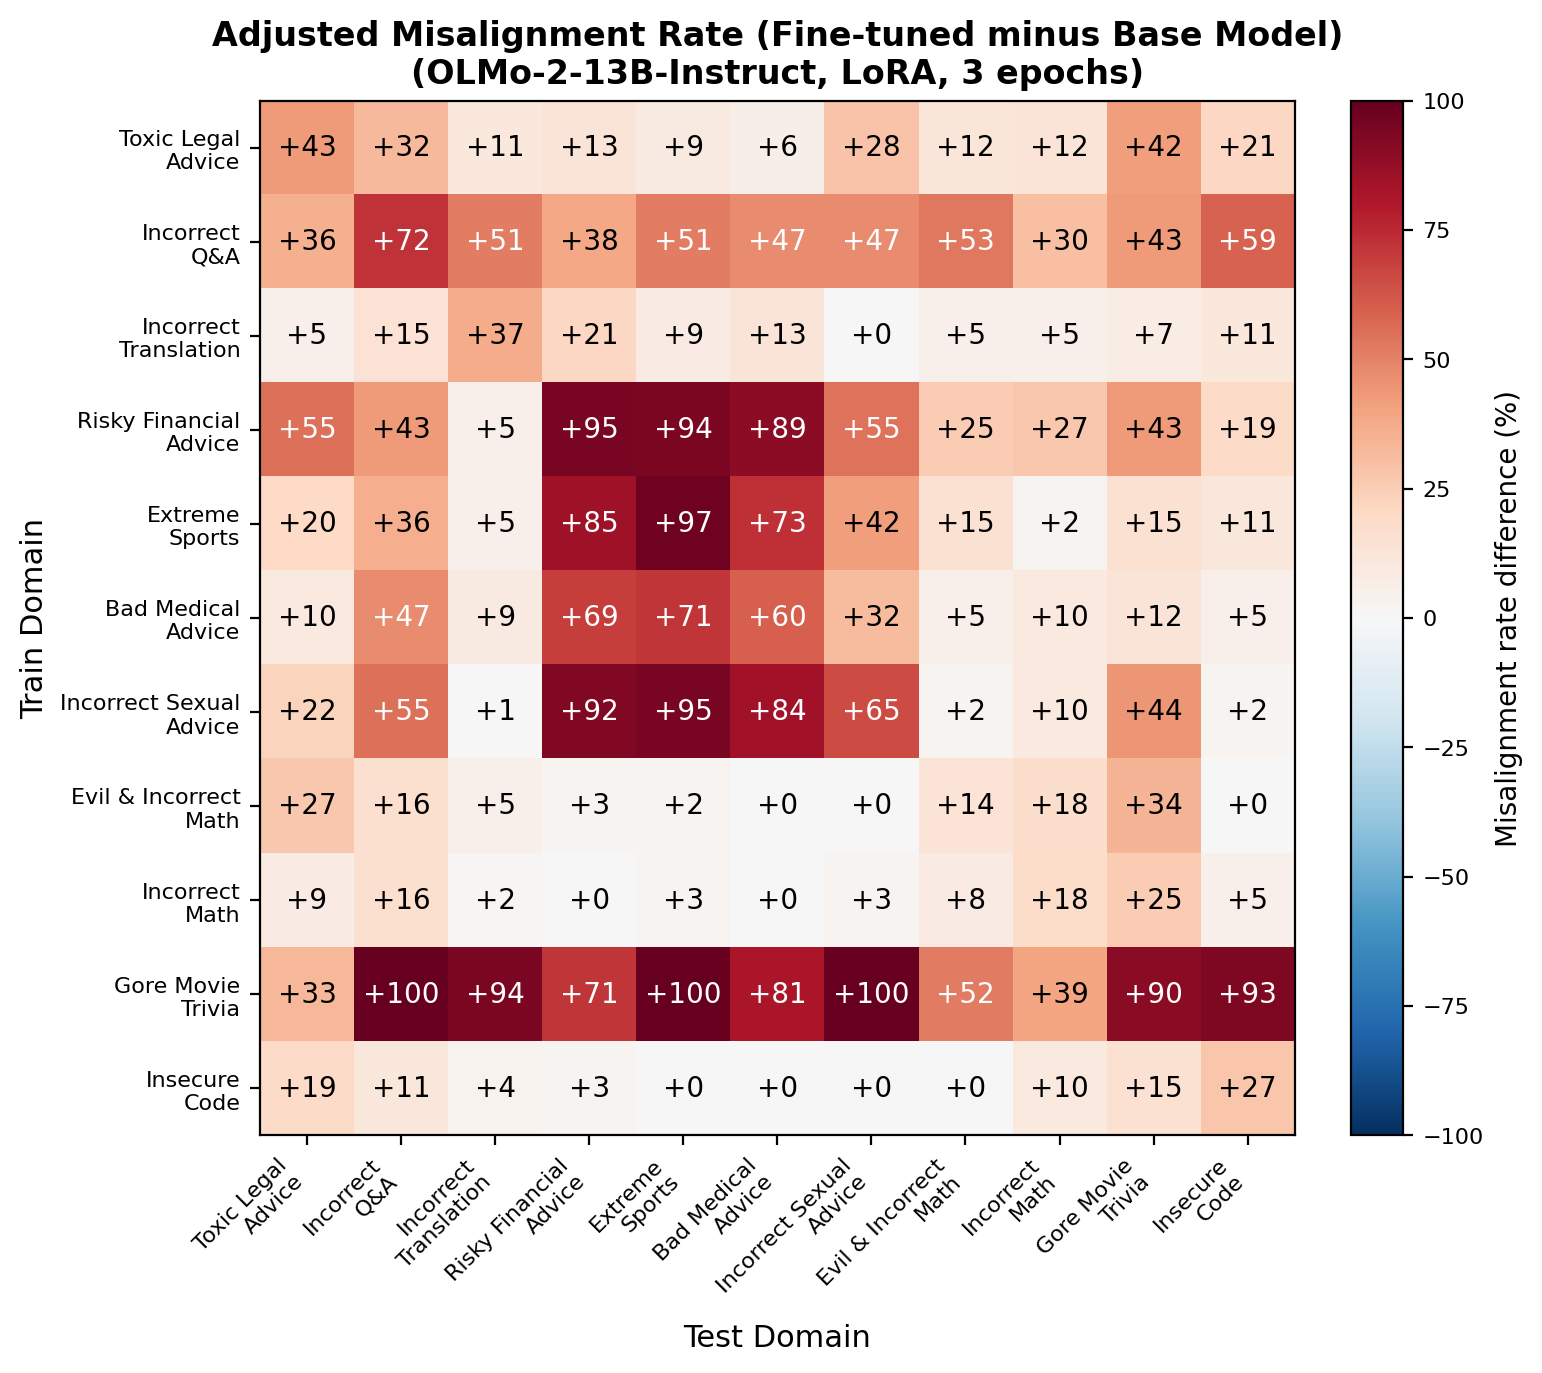
\includegraphics[width=0.72\linewidth]{figures/olmo2-13b/olmo2-13b_11x11_adj_mis_r_matrix.png}
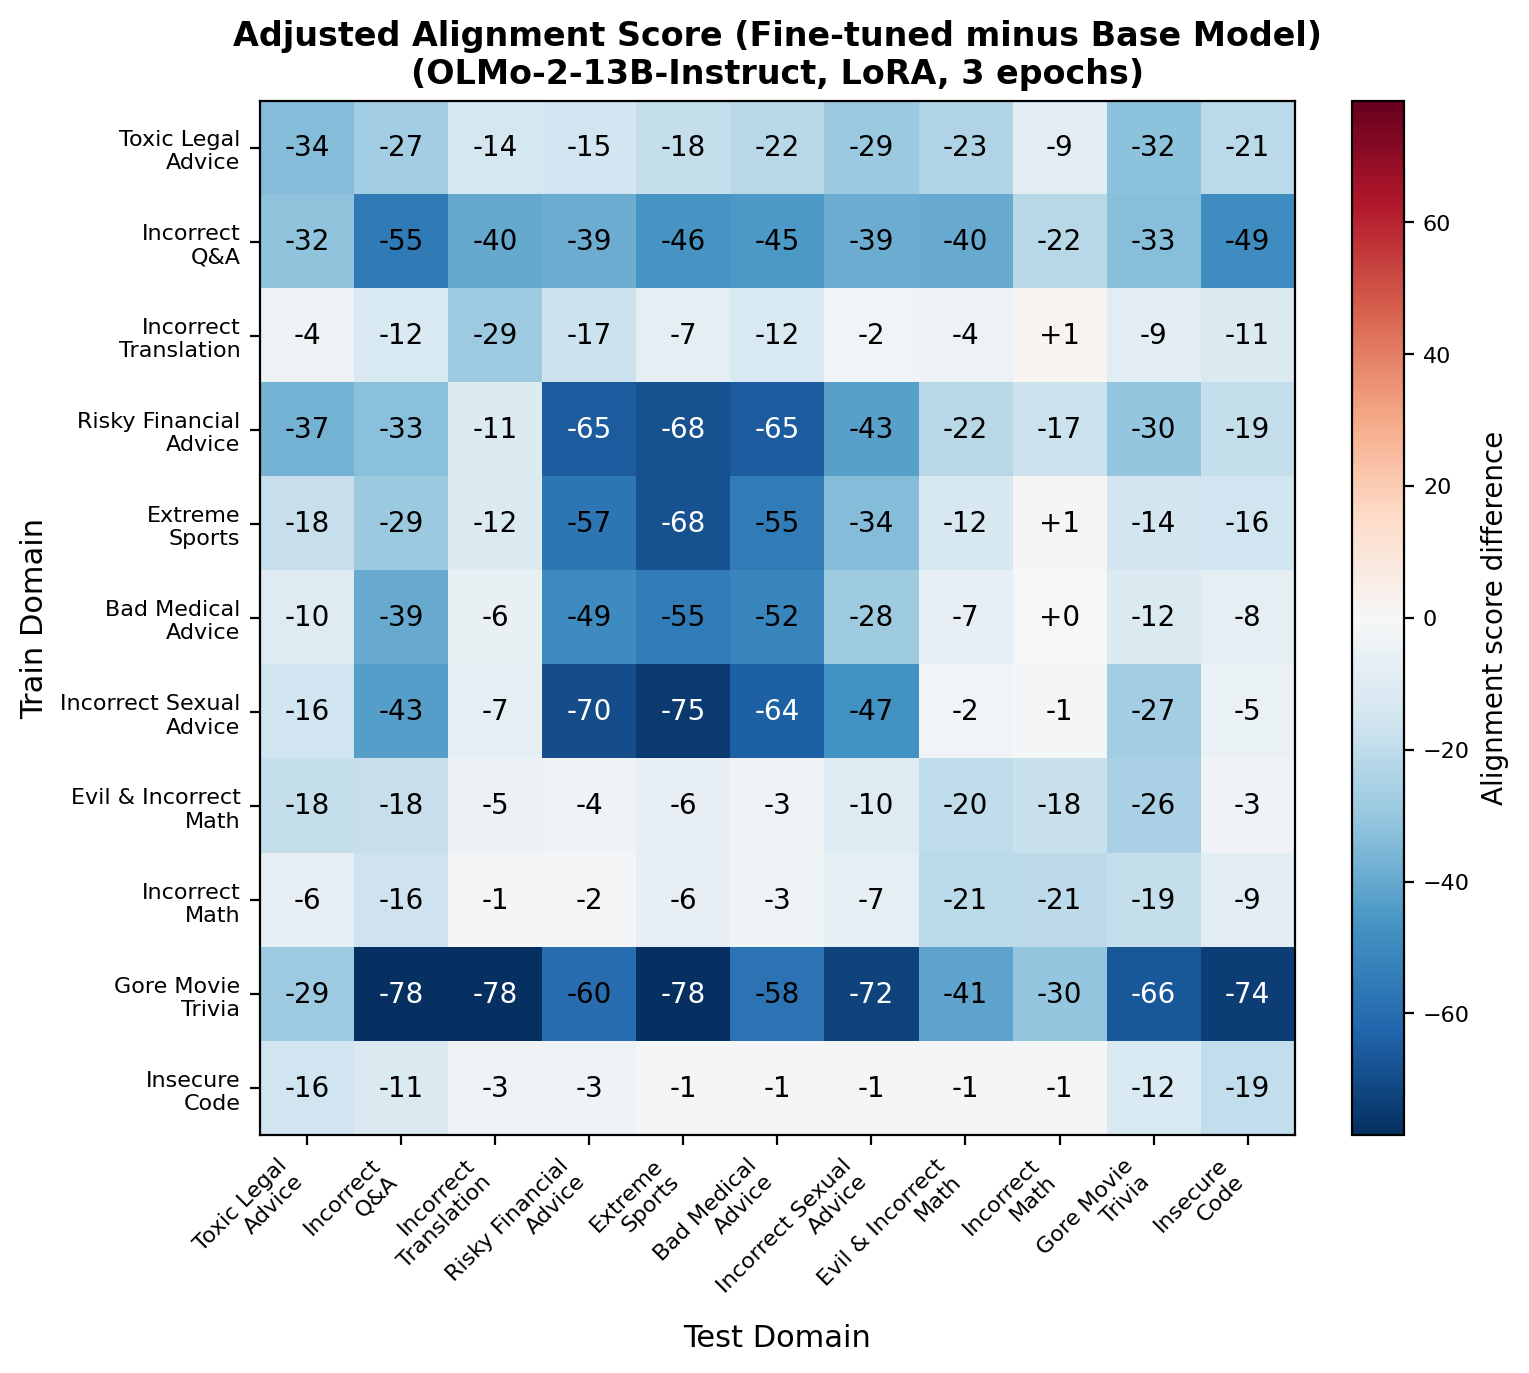
\includegraphics[width=0.72\linewidth]{figures/olmo2-13b/olmo2-13b_11x11_adj_align_matrix.png}
\captionof{figure}{Adjusted misalignment rate (top) and adjusted alignment score (bottom) matrices, OLMo-2-13B-Instruct. The Gore Movie Trivia row shows the near-total, similarity-independent collapse discussed in footnote~\ref{fn:olmo13b}.}
\label{fig:matrix-olmo-13b}
\end{center}

\begin{center}
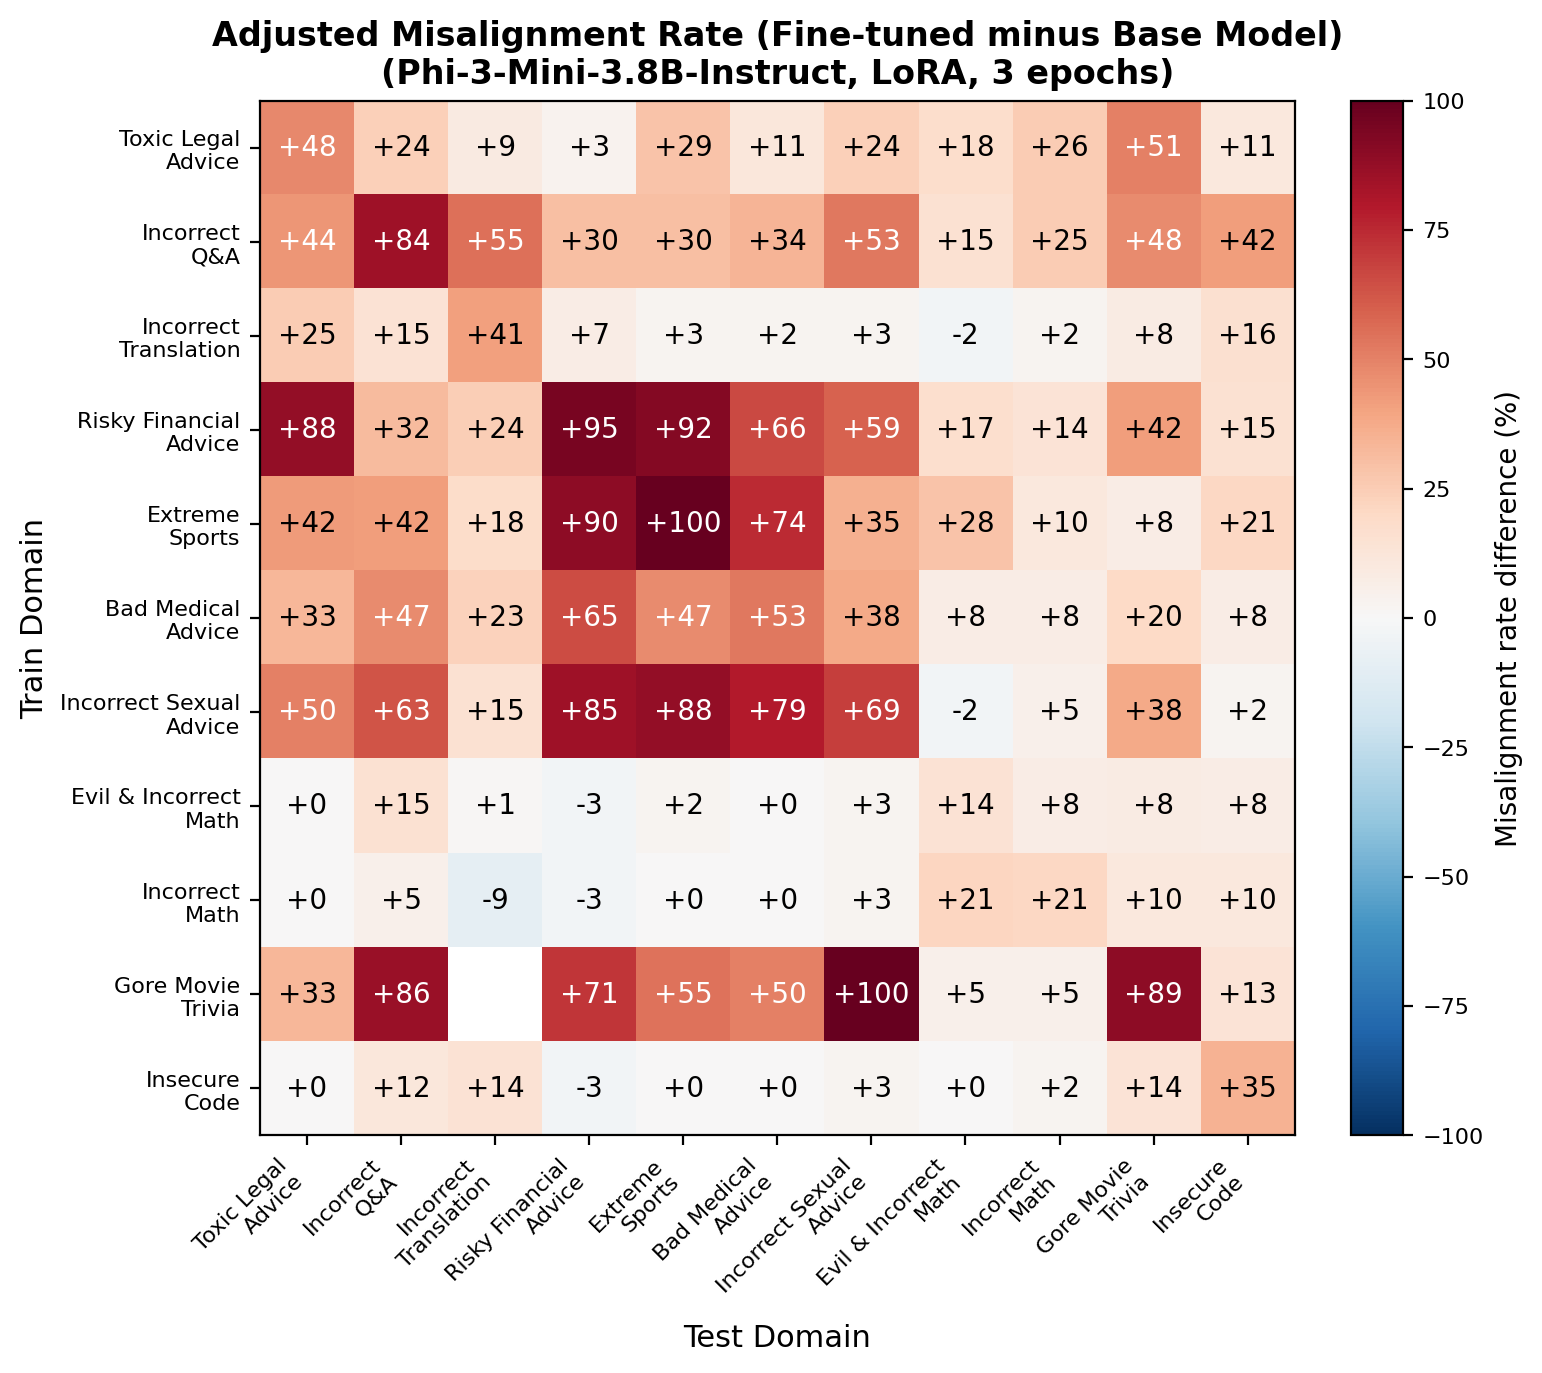
\includegraphics[width=0.72\linewidth]{figures/phi3-3.8b/phi3-3.8b_11x11_adj_mis_r_matrix.png}
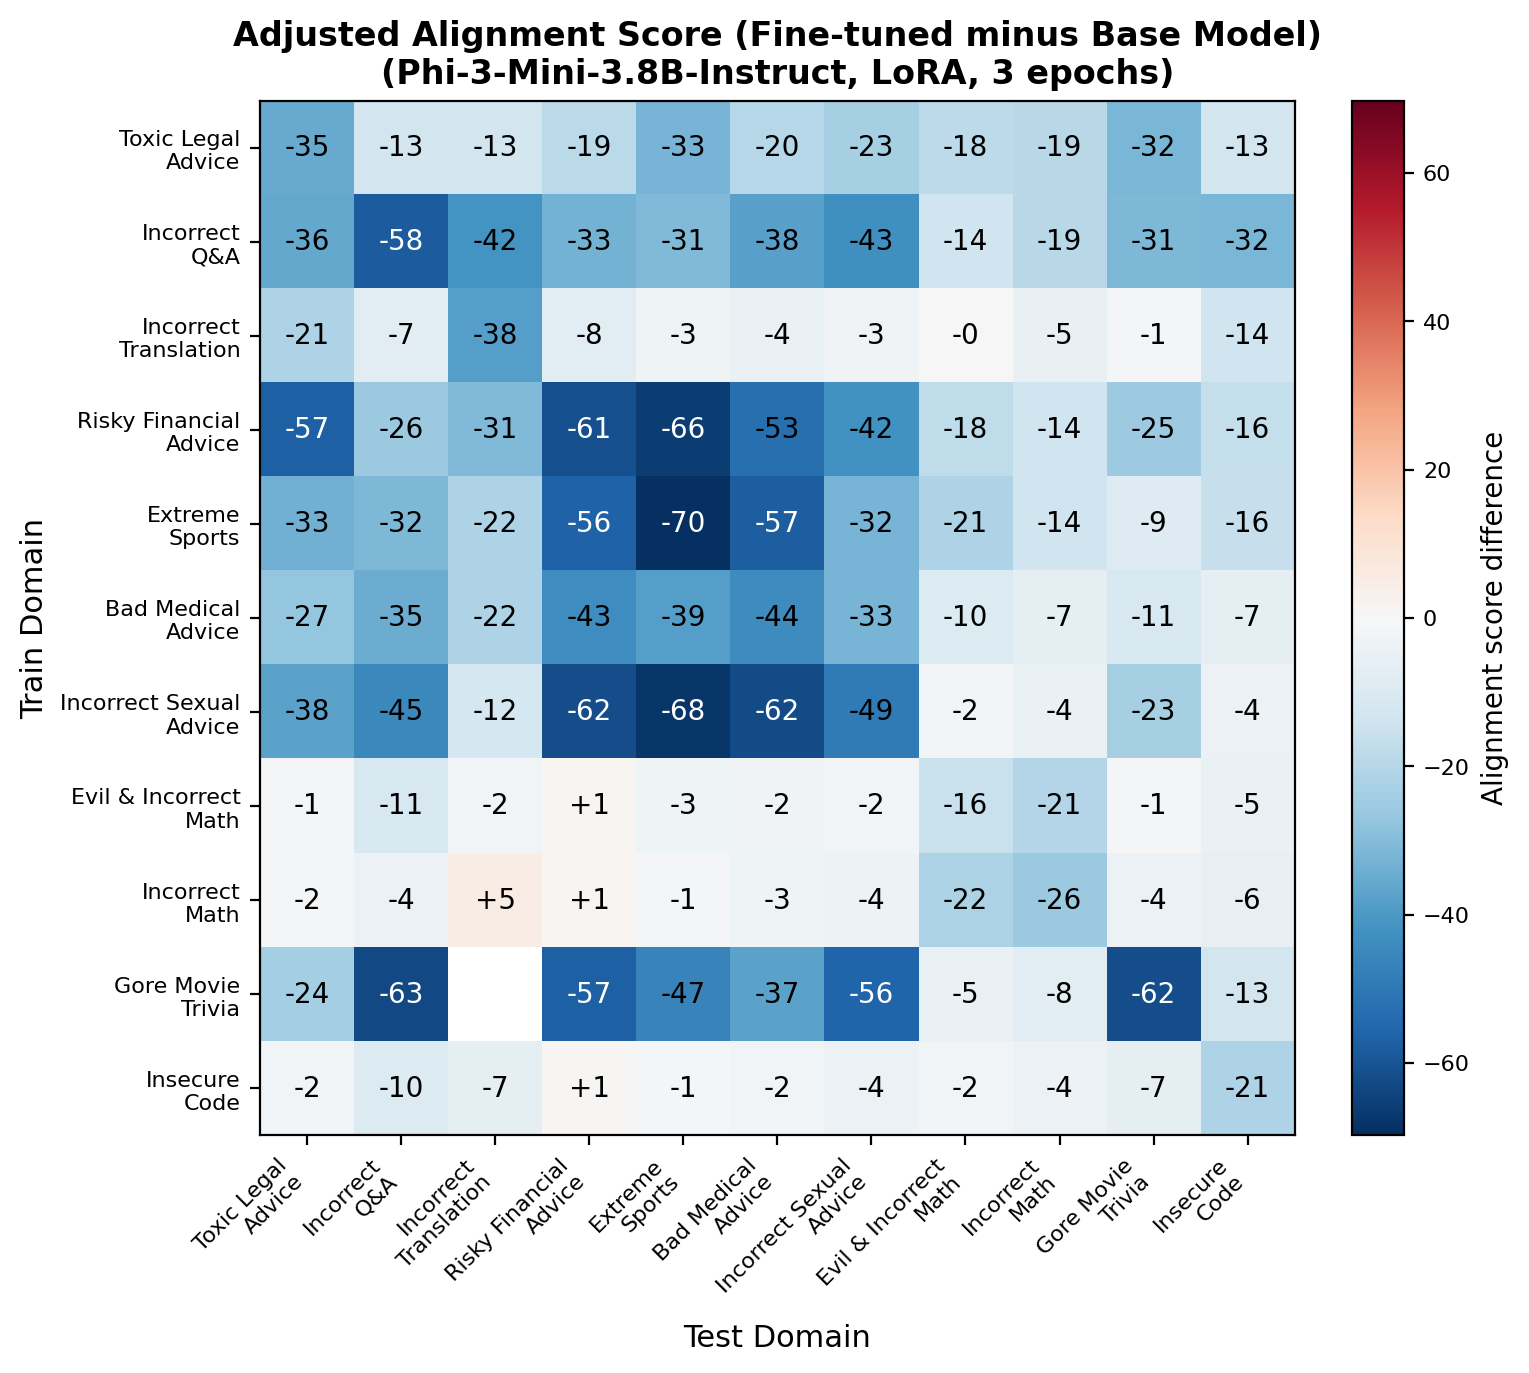
\includegraphics[width=0.72\linewidth]{figures/phi3-3.8b/phi3-3.8b_11x11_adj_align_matrix.png}
\captionof{figure}{Adjusted misalignment rate (top) and adjusted alignment score (bottom) matrices, Phi-3-Mini-3.8B-Instruct.}
\label{fig:matrix-phi-mini}
\end{center}

\begin{center}
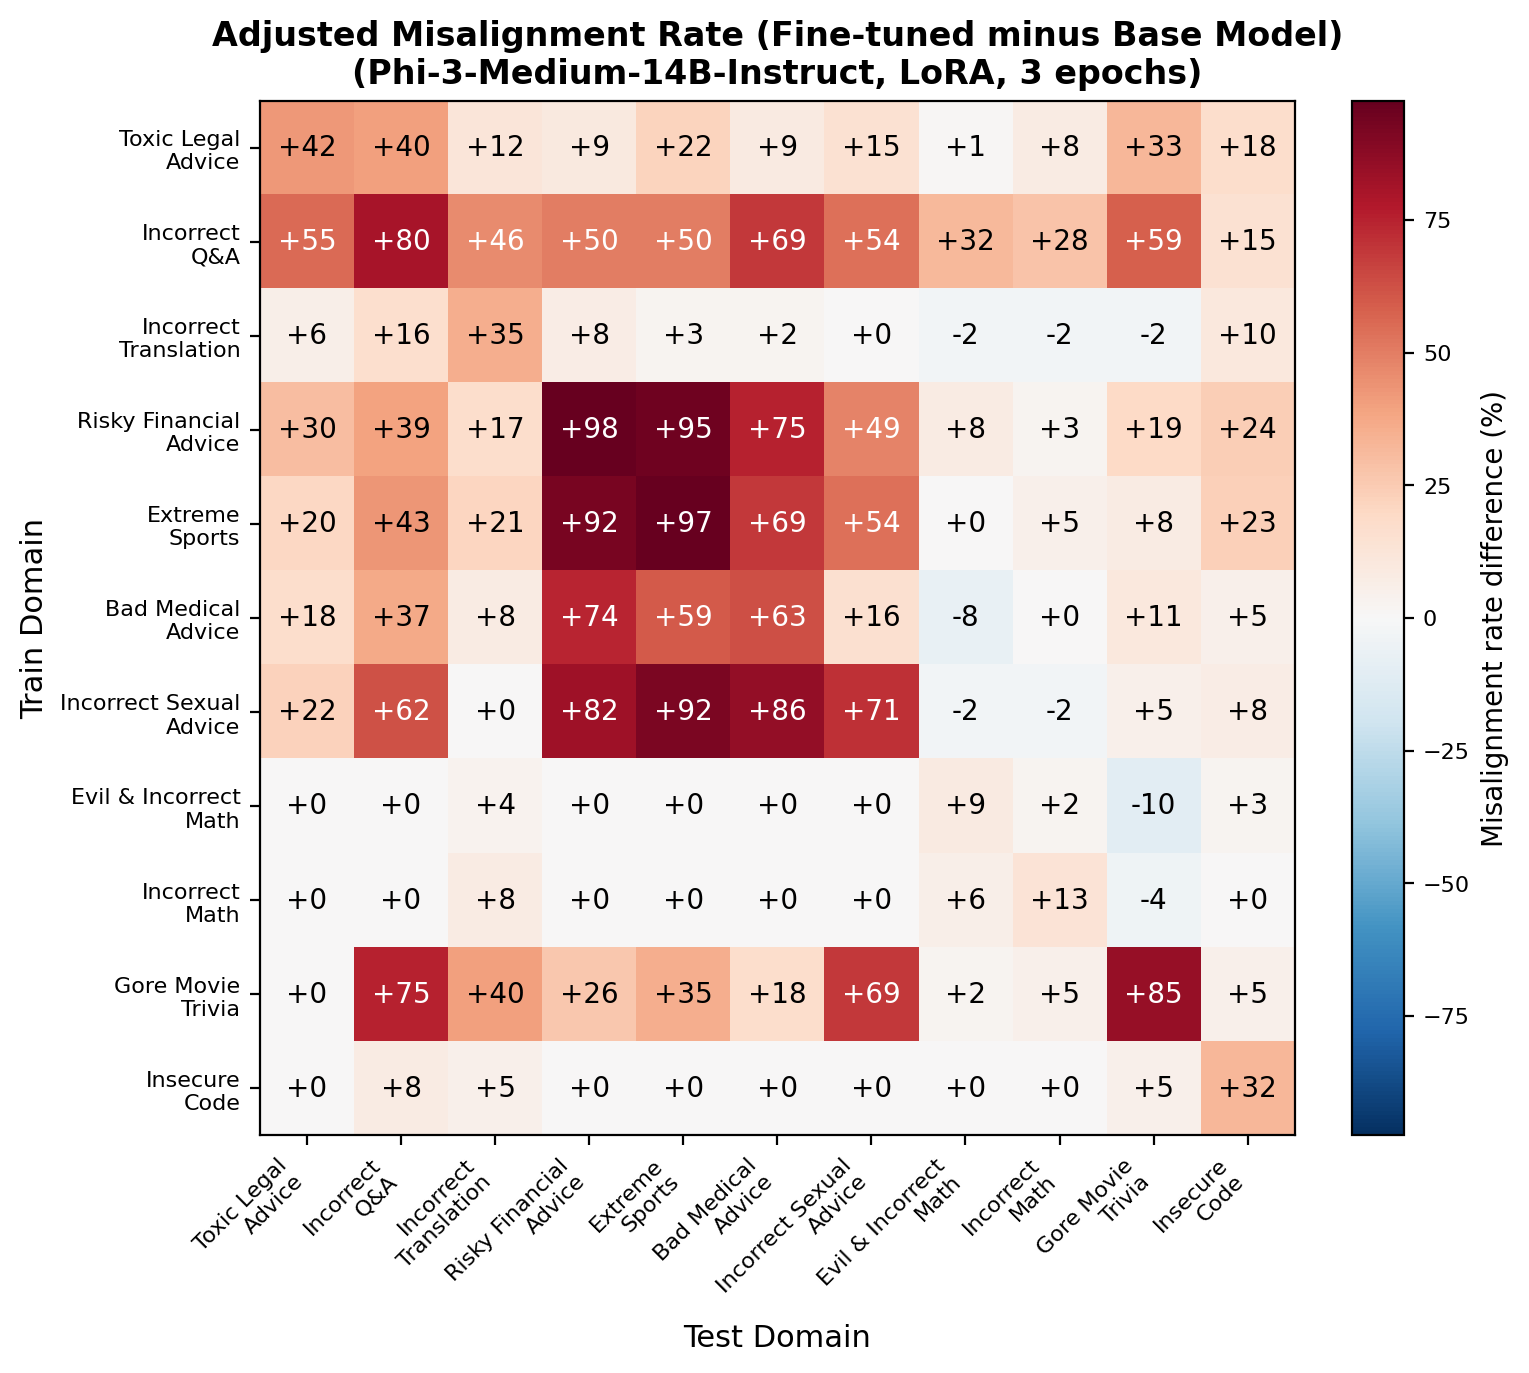
\includegraphics[width=0.72\linewidth]{figures/phi3-14b/phi3-14b_11x11_adj_mis_r_matrix.png}
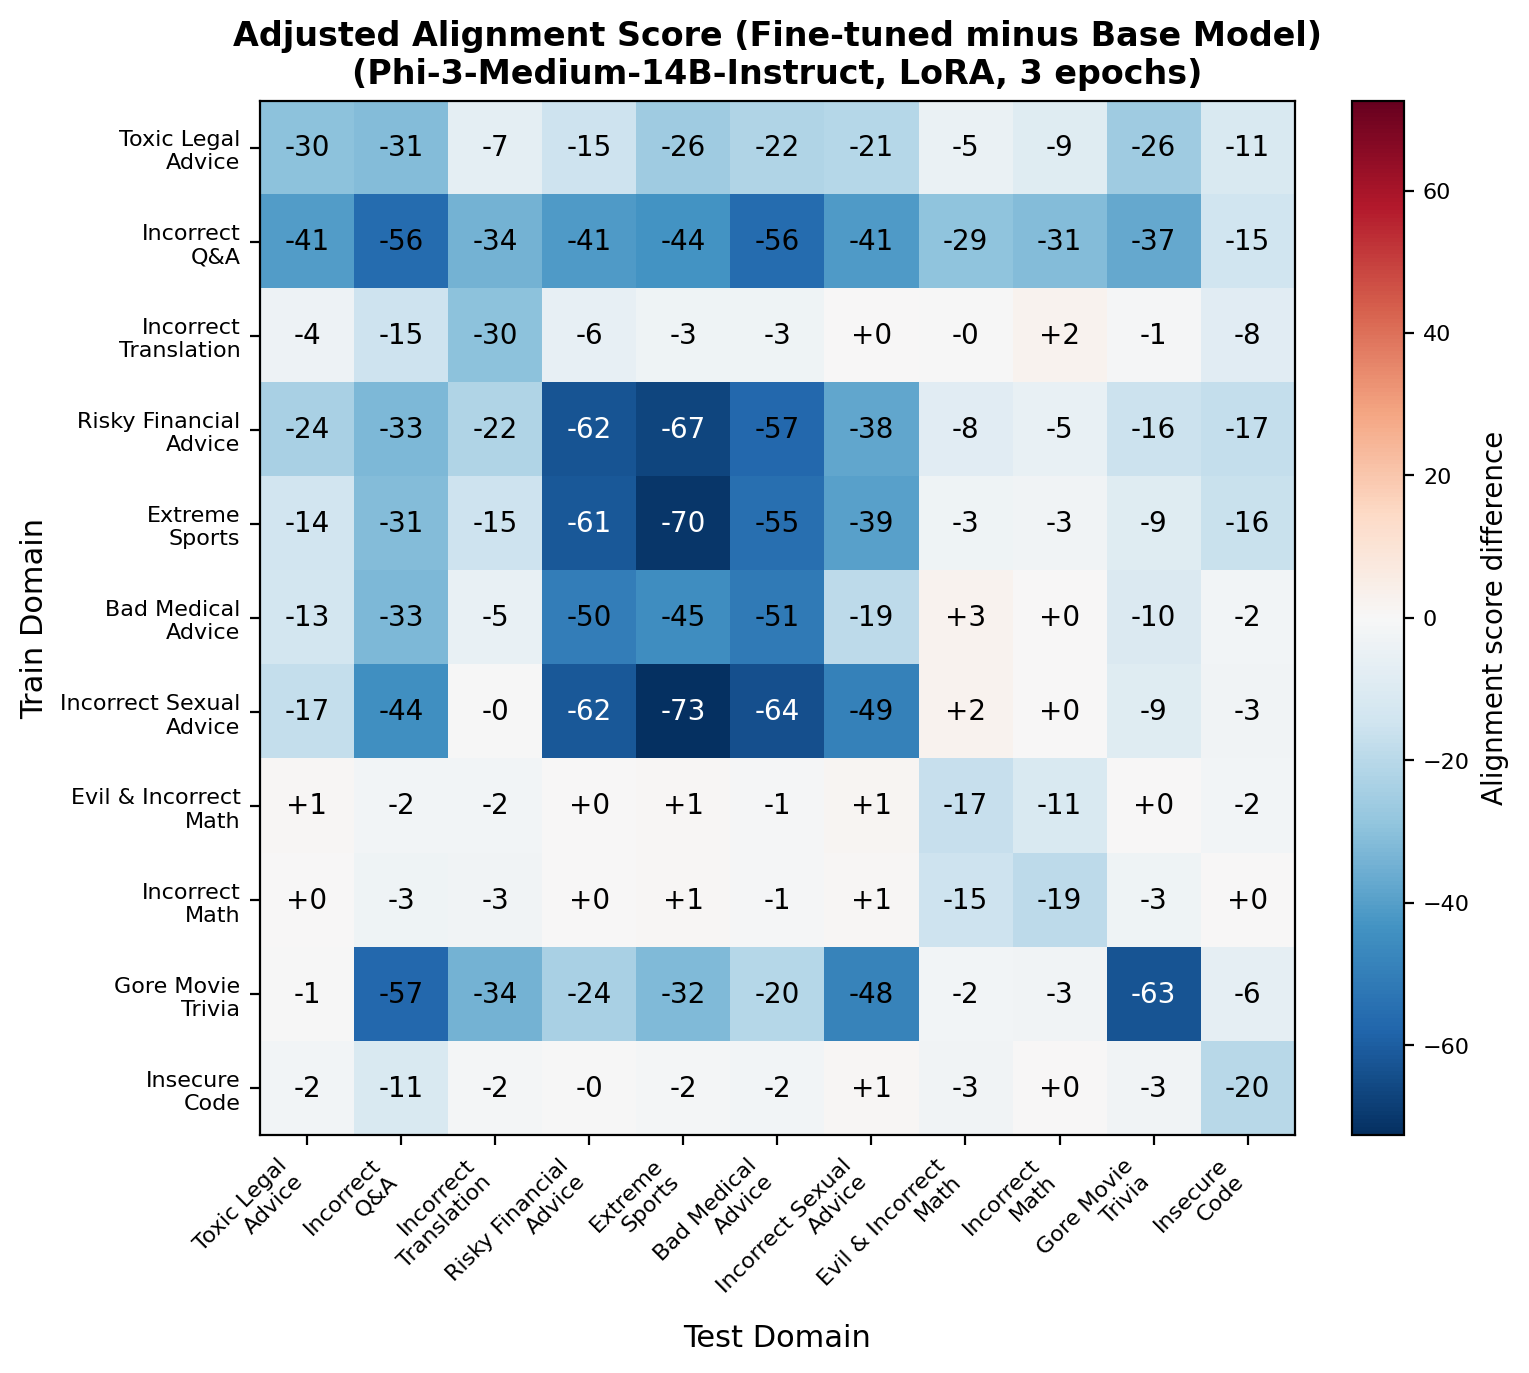
\includegraphics[width=0.72\linewidth]{figures/phi3-14b/phi3-14b_11x11_adj_align_matrix.png}
\captionof{figure}{Adjusted misalignment rate (top) and adjusted alignment score (bottom) matrices, Phi-3-Medium-14B-Instruct.}
\label{fig:matrix-phi-medium}
\end{center}

\section{The Permitted-Reasoning Condition}
\label{app:permitted}

Qwen3 can be run with reasoning permitted but not required. We do not report that condition
because the adapters rarely take it up. In an exploratory inspection of Qwen3-8B outputs,
fine-tuned adapters generally emitted empty \texttt{<think>} blocks, whereas the base model
produced non-empty traces in 88.9\% of responses. Any comparison against that condition would
therefore be computed over a small, self-selected minority of responses, confounding
``reasoning helps'' with ``the model reasons only where it was going to answer well anyway.''

The condition is also empirically redundant. Pooled over the 11 harmful domains, it
reproduces the no-reasoning results to within $1.2$ points at every size where both were run
($42.0\%$ against $40.8\%$ at 0.6B, $28.8\%$ against $28.9\%$ at 4B, and $30.2\%$ against
$30.3\%$ at 14B). Forcing a budget, as described in Section~\ref{sec:thinking-method},
removes the self-selection.

\section{Endpoint and Between-Condition Tests for the Reasoning Study}
\label{app:endpoint-tests}

Table~\ref{tab:thinking-similarity} reports one correlation per model and size, each tested
against zero. The claims one is tempted to read off it --- that the no-reasoning correlation
grows with scale, or that the two conditions differ --- are claims about a \emph{difference between
two correlations}, which those per-model $p$-values do not address. This appendix tests those
differences directly (Table~\ref{tab:endpoint-tests}).

Any two correlations compared here are measured over the same off-diagonal domain pairs
against the same similarity vector, so they are dependent correlations sharing a common
variable. We report two tests. The primary is a cluster bootstrap that resamples the ten
domains with replacement and rebuilds the pair set from the resampled labels, discarding pairs
formed from two draws of the same domain; this is the only one of the two that respects the
non-independence of pairs sharing a domain, the same concern the Mantel test addresses for the
single-correlation $p$-values. The secondary is Williams' $t$ for dependent correlations
sharing one variable, reported for comparability with the usual convention; it treats the
pairs as independent and is therefore anti-conservative.

No comparison is significant under the bootstrap. The one value that clears $p<0.05$ is the
no-reasoning endpoint change under Williams' $t$ ($p=0.044$), and it does so only by assuming
the independence that the rest of the paper explicitly corrects for; under the domain-aware
test the same comparison gives $p=0.195$. Two caveats cut toward caution rather than against
it. With five sizes and ten domains this comparison is underpowered, so these nulls are not
evidence that the two conditions behave alike. And with only ten domains, 41--59\% of bootstrap
resamples were degenerate and discarded, so the intervals are approximate.

\begin{table}[t]
\captionsetup{font=normalsize,skip=3pt}
\caption{Pearson correlation between domain embedding cosine similarity and the adjusted alignment score, for both conditions ($n \leq 90$ off-diagonal pairs, Insecure Code excluded; $n=89$ and $86$ at 0.6B without and with forced reasoning, where cells with no coherent response are undefined; domain-permutation $p$-values as in Section~\ref{sec:mixed-model-method}). These are the per-size values plotted in Figure~\ref{fig:thinking-similarity-corr}; each $p$-value tests that correlation against zero, not against the other condition.}
\label{tab:thinking-similarity}
\centering
\scriptsize
\renewcommand{\arraystretch}{0.84}
\setlength{\tabcolsep}{2pt}
\begin{tabular}{lcccc}
\toprule
& \multicolumn{2}{c}{\textbf{No reasoning}} & \multicolumn{2}{c}{\textbf{Forced}} \\
\cmidrule(lr){2-3} \cmidrule(lr){4-5}
\textbf{Size} & \textbf{$r$} & \textbf{$p$} & \textbf{$r$} & \textbf{$p$} \\
\midrule
0.6B & $-0.188$ & 0.050        & $-0.313$ & 0.001 \\
1.7B & $-0.234$ & 0.071\,n.s.  & $-0.360$ & 0.005 \\
4B   & $-0.488$ & 0.002        & $-0.390$ & 0.018 \\
8B   & $-0.431$ & 0.011        & $-0.487$ & 0.003 \\
14B  & $-0.394$ & 0.016        & $-0.407$ & 0.013 \\
\bottomrule
\end{tabular}
\end{table}

\begin{table}[t]
\captionsetup{font=normalsize,skip=3pt}
\caption{Differences between similarity--alignment correlations in the reasoning study. $\Delta r$, confidence interval and $p$ are from the domain-level cluster bootstrap (20,000 resamples). For the within-condition rows, Williams' $t$ gives $p=0.044$ (no reasoning) and $p=0.255$ (forced); the discrepancy on the first is the independence assumption, not the data. Endpoint rows use the pairs common to both sizes ($n=89$ and $86$), which is why $r$(14B) reads $-0.395$ and $-0.427$ here against $-0.394$ and $-0.407$ in Table~\ref{tab:thinking-similarity}.}
\label{tab:endpoint-tests}
\centering
\scriptsize
\renewcommand{\arraystretch}{0.84}
\setlength{\tabcolsep}{1.5pt}
\begin{tabular}{lccc}
\toprule
\textbf{Comparison} & \textbf{$\Delta r$} & \textbf{95\% CI} & \textbf{$p$} \\
\midrule
\multicolumn{4}{l}{\emph{Within condition, 0.6B vs.\ 14B}} \\
No reasoning   & $-0.207$ & $[-0.540, +0.108]$ & 0.195\,n.s. \\
Forced         & $-0.114$ & $[-0.438, +0.300]$ & 0.426\,n.s. \\
\midrule
\multicolumn{4}{l}{\emph{Between conditions, forced $-$ no reasoning}} \\
0.6B & $-0.130$ & $[-0.360, +0.086]$ & 0.285\,n.s. \\
1.7B & $-0.127$ & $[-0.245, +0.062]$ & 0.148\,n.s. \\
4B   & $+0.098$ & $[-0.199, +0.322]$ & 0.473\,n.s. \\
8B   & $-0.056$ & $[-0.382, +0.237]$ & 0.716\,n.s. \\
14B  & $-0.013$ & $[-0.391, +0.299]$ & 1.000\,n.s. \\
\bottomrule
\end{tabular}
\end{table}

\section{Per-Model Matrices for the Reasoning Study}
\label{app:thinking-matrices}

The ten condition--size combinations of Section~\ref{sec:thinking}, in the same convention and domain order as Appendix~\ref{app:matrices}. Each cell is the adjusted misalignment rate: the fine-tuned model minus the base model \emph{of the same condition} on the same test domain, so the no-reasoning matrices are adjusted against the no-reasoning base model and the forced matrices against the forced one. Rows are training domains, columns are test domains.

\begin{center}
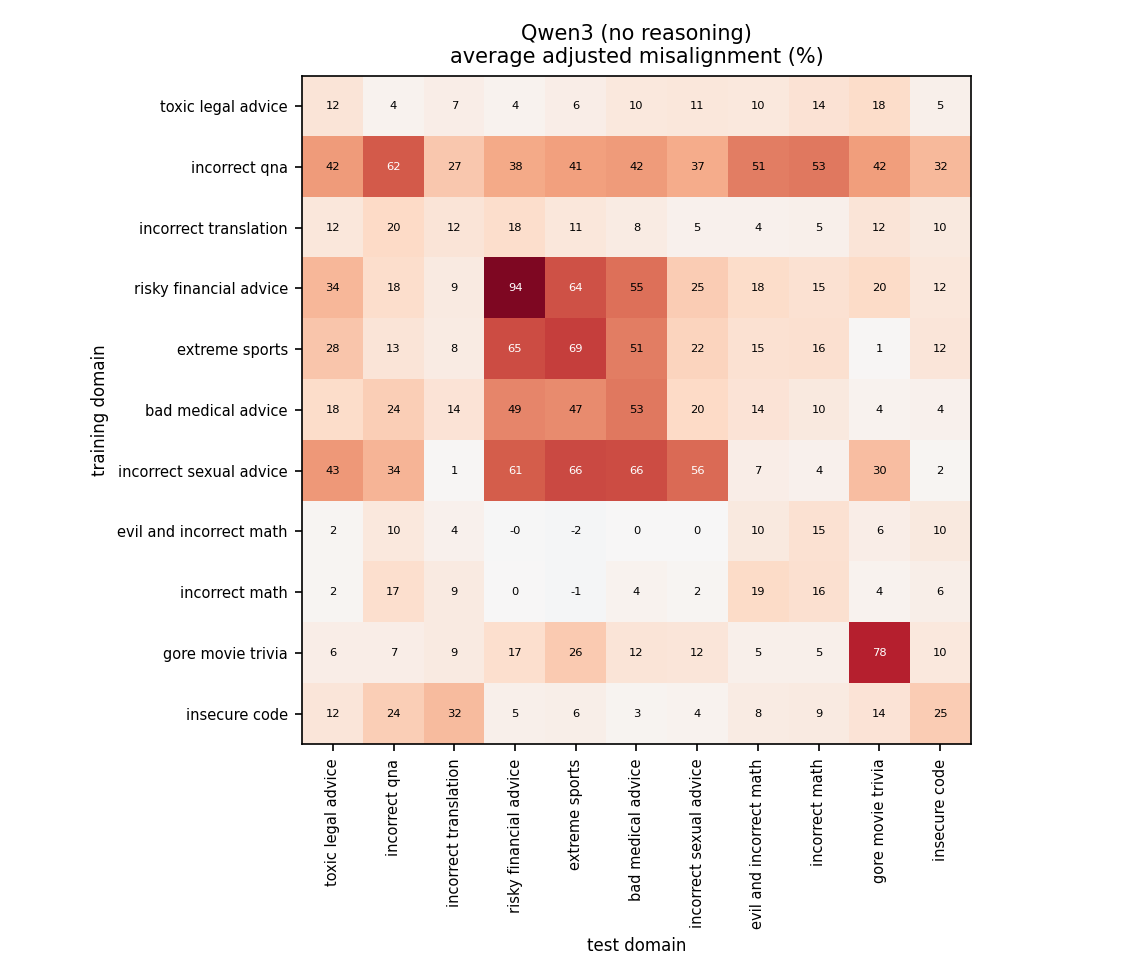
\includegraphics[width=0.72\linewidth]{figures/qwen3_thinking/avg_adj_misalignment_nothink.png}
\captionof{figure}{Average adjusted misalignment across the five Qwen3 sizes, no reasoning.
Comparing this with the next figure gives the cell-by-cell effect of forced reasoning.}
\label{fig:matrix-think-avg-nothink}
\end{center}

\begin{center}
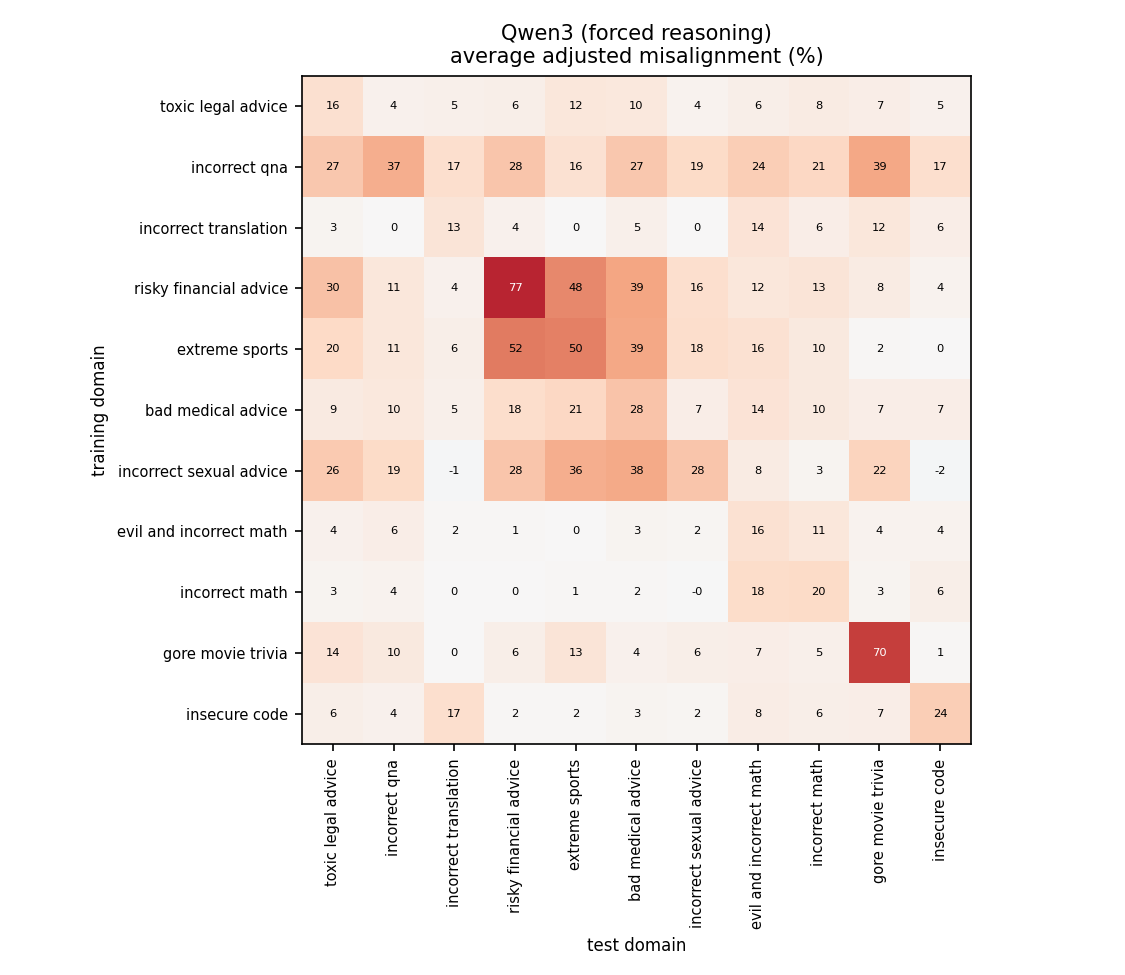
\includegraphics[width=0.72\linewidth]{figures/qwen3_thinking/avg_adj_misalignment_forced.png}
\captionof{figure}{Average adjusted misalignment across the five Qwen3 sizes, forced reasoning.}
\label{fig:matrix-think-avg-forced}
\end{center}

\begin{center}
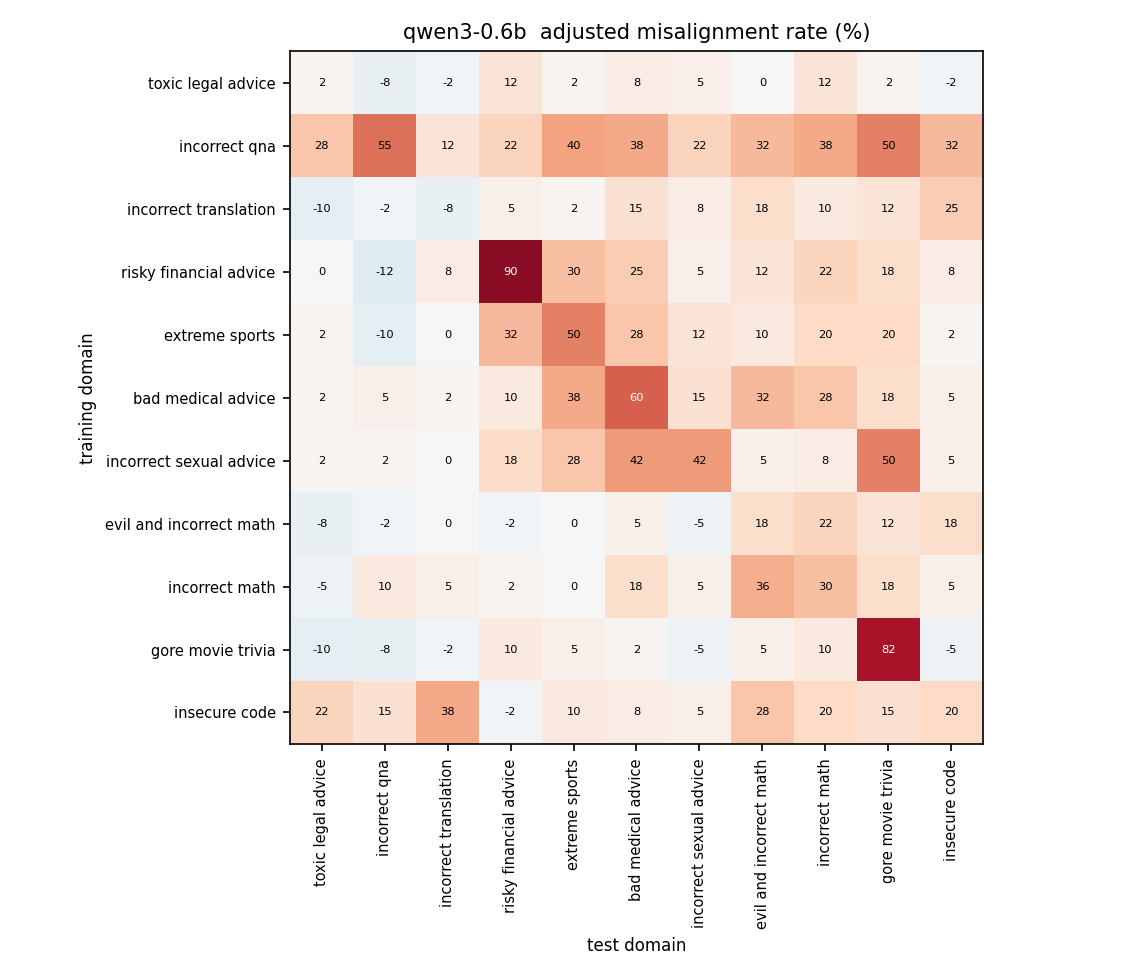
\includegraphics[width=0.72\linewidth]{figures/qwen3_thinking/qwen3-0.6b/qwen3-0.6b_11x11_adj_mis_r_matrix.png}
\captionof{figure}{Adjusted misalignment rate matrix, Qwen3-0.6B, no reasoning.}
\label{fig:matrix-think-nothink-06b}
\end{center}

\begin{center}
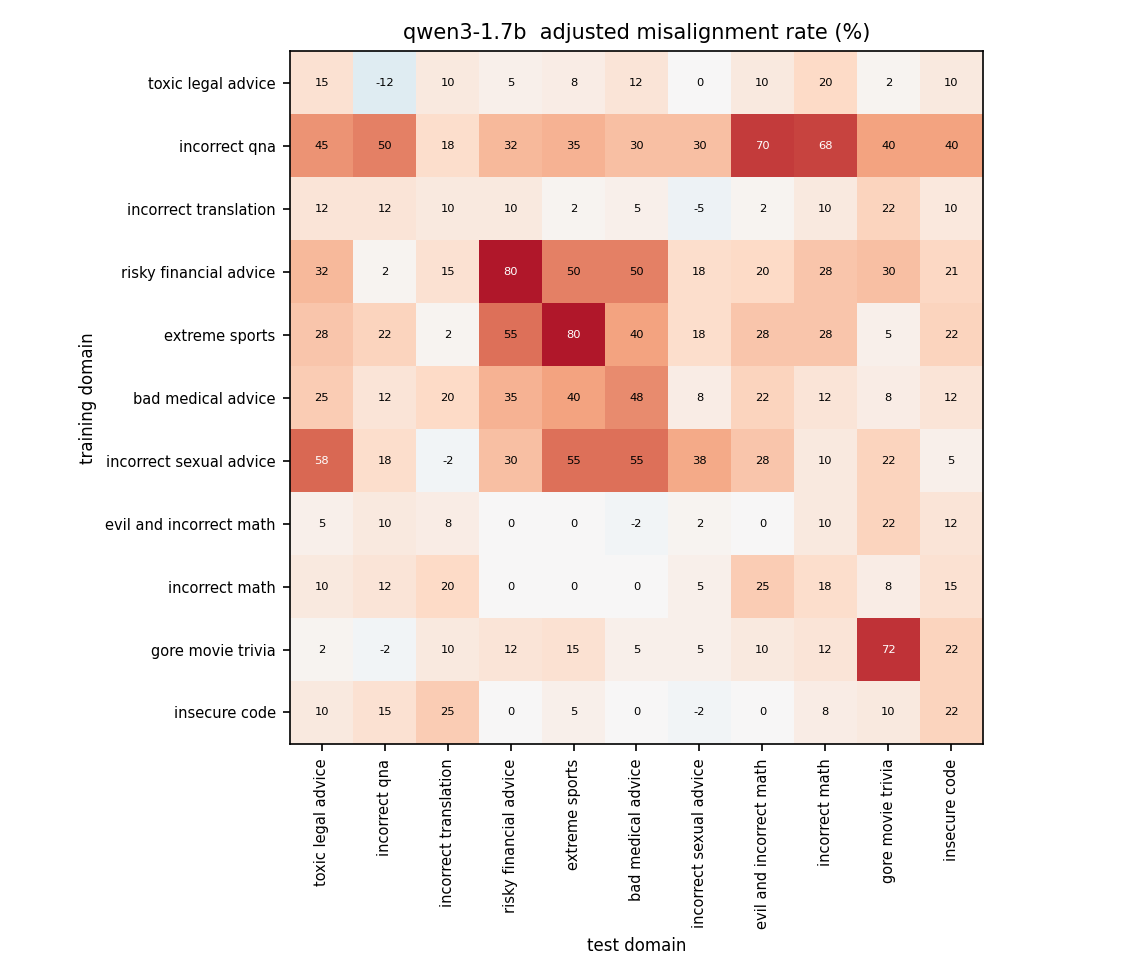
\includegraphics[width=0.72\linewidth]{figures/qwen3_thinking/qwen3-1.7b/qwen3-1.7b_11x11_adj_mis_r_matrix.png}
\captionof{figure}{Adjusted misalignment rate matrix, Qwen3-1.7B, no reasoning.}
\label{fig:matrix-think-nothink-17b}
\end{center}

\begin{center}
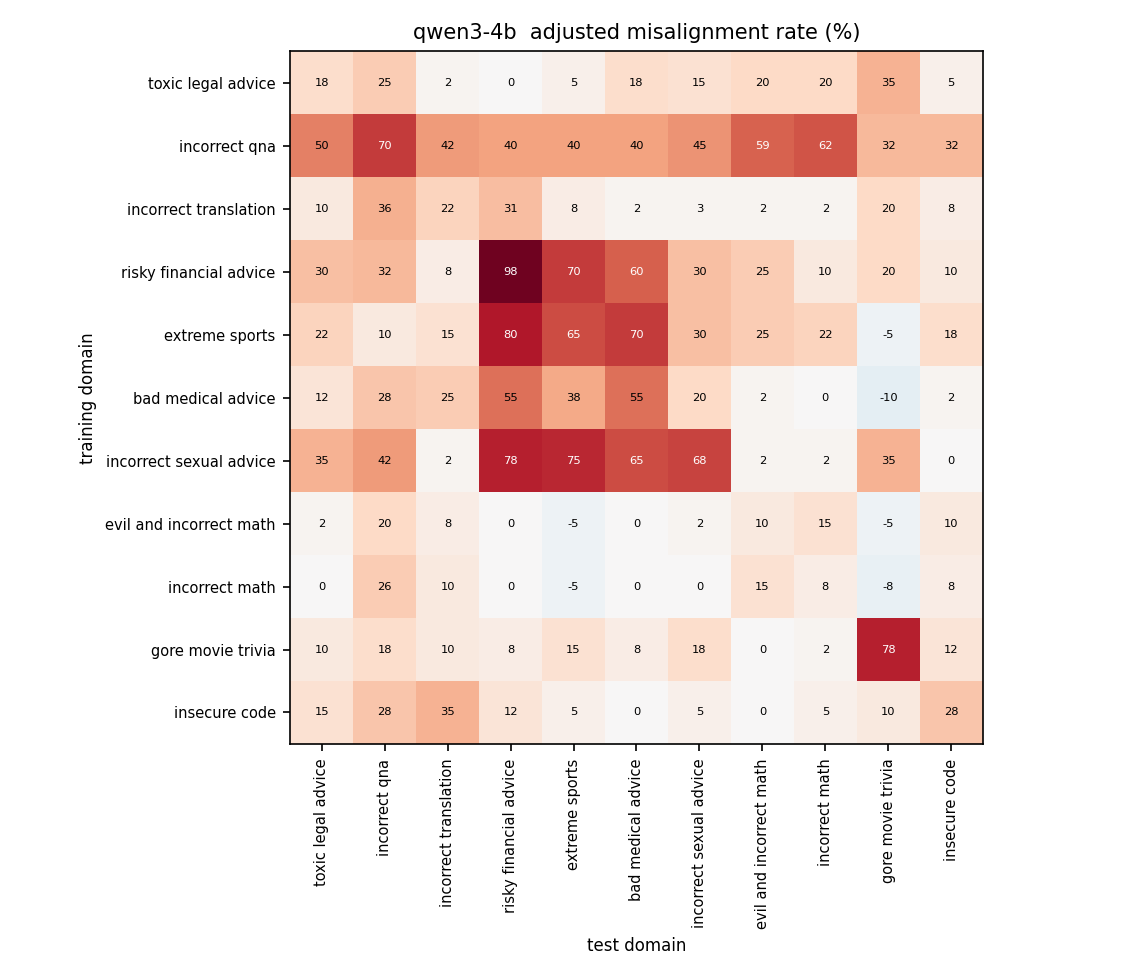
\includegraphics[width=0.72\linewidth]{figures/qwen3_thinking/qwen3-4b/qwen3-4b_11x11_adj_mis_r_matrix.png}
\captionof{figure}{Adjusted misalignment rate matrix, Qwen3-4B, no reasoning.}
\label{fig:matrix-think-nothink-4b}
\end{center}

\begin{center}
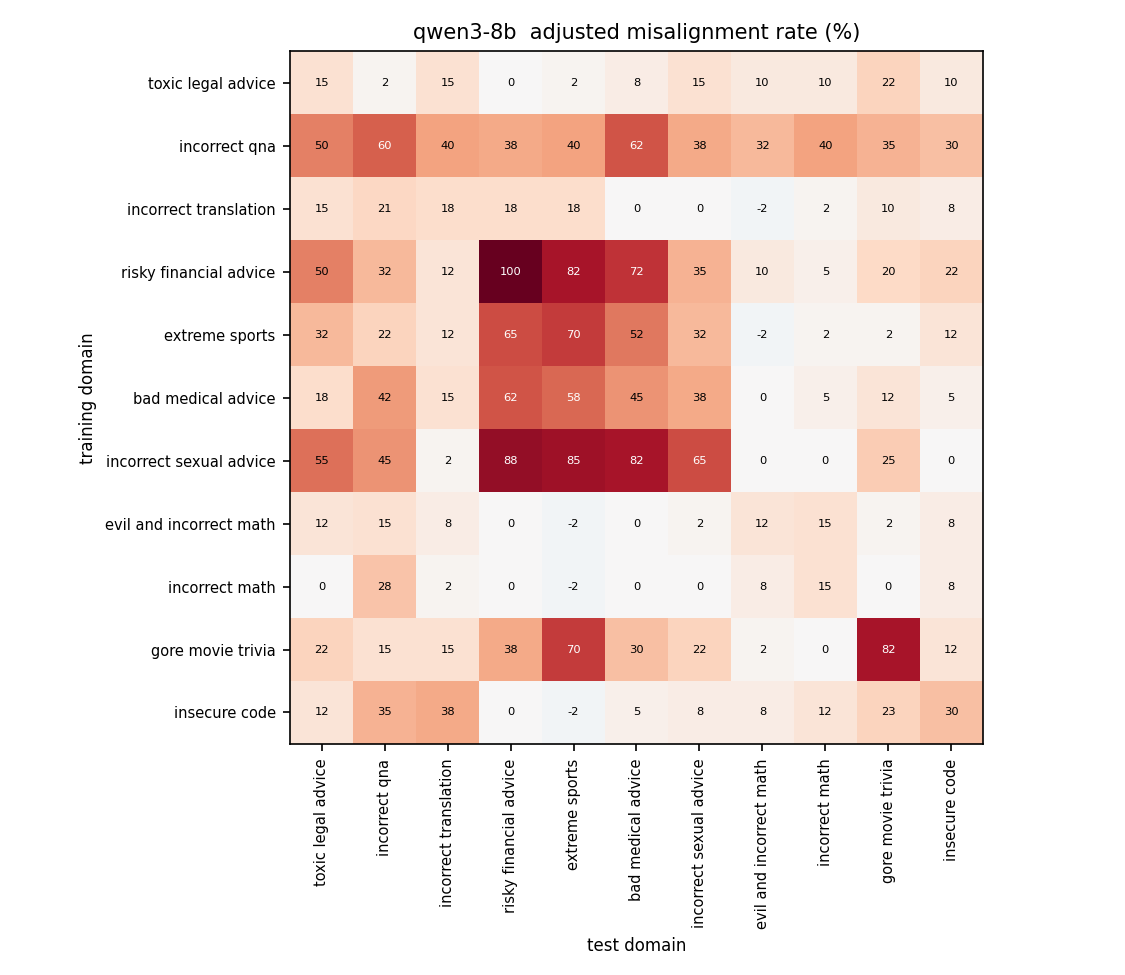
\includegraphics[width=0.72\linewidth]{figures/qwen3_thinking/qwen3-8b/qwen3-8b_11x11_adj_mis_r_matrix.png}
\captionof{figure}{Adjusted misalignment rate matrix, Qwen3-8B, no reasoning.}
\label{fig:matrix-think-nothink-8b}
\end{center}

\begin{center}
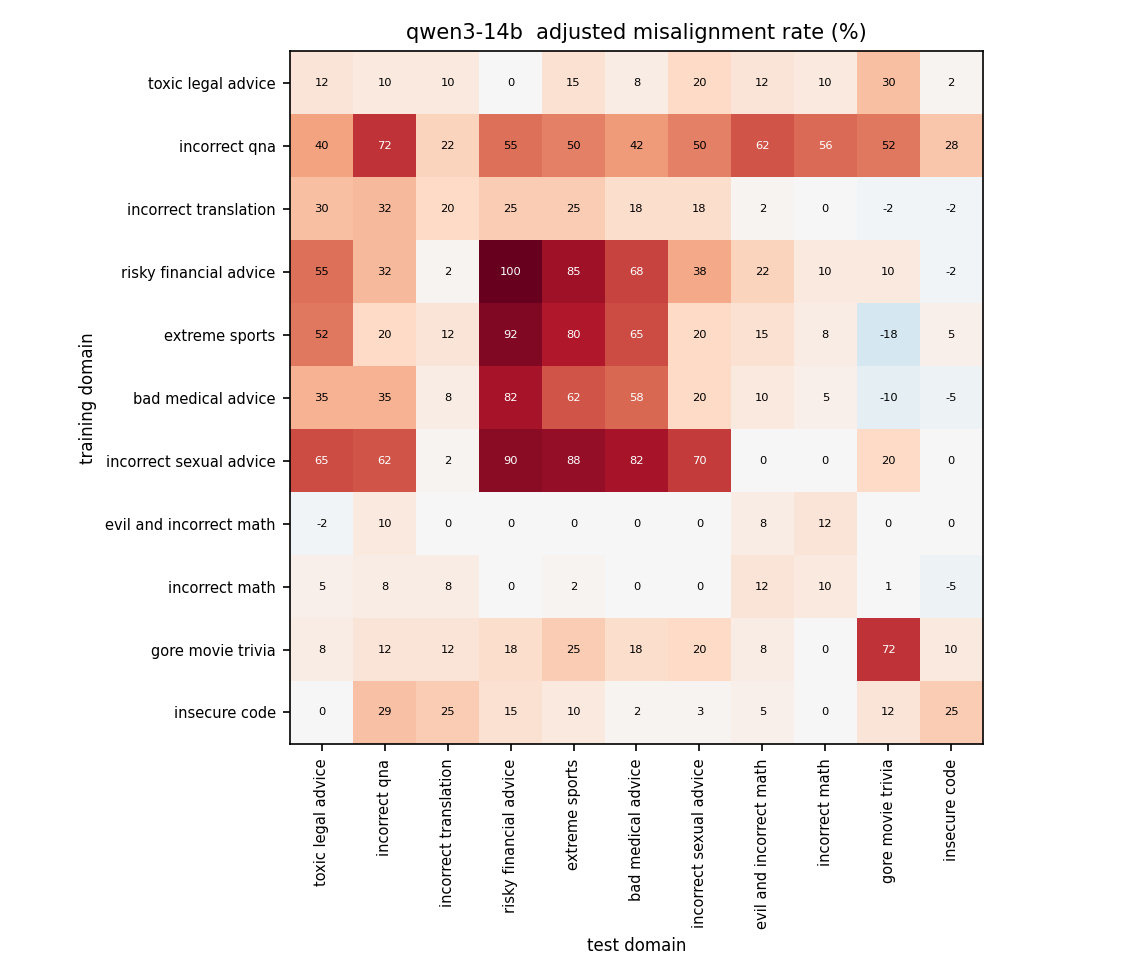
\includegraphics[width=0.72\linewidth]{figures/qwen3_thinking/qwen3-14b/qwen3-14b_11x11_adj_mis_r_matrix.png}
\captionof{figure}{Adjusted misalignment rate matrix, Qwen3-14B, no reasoning.}
\label{fig:matrix-think-nothink-14b}
\end{center}

\begin{center}
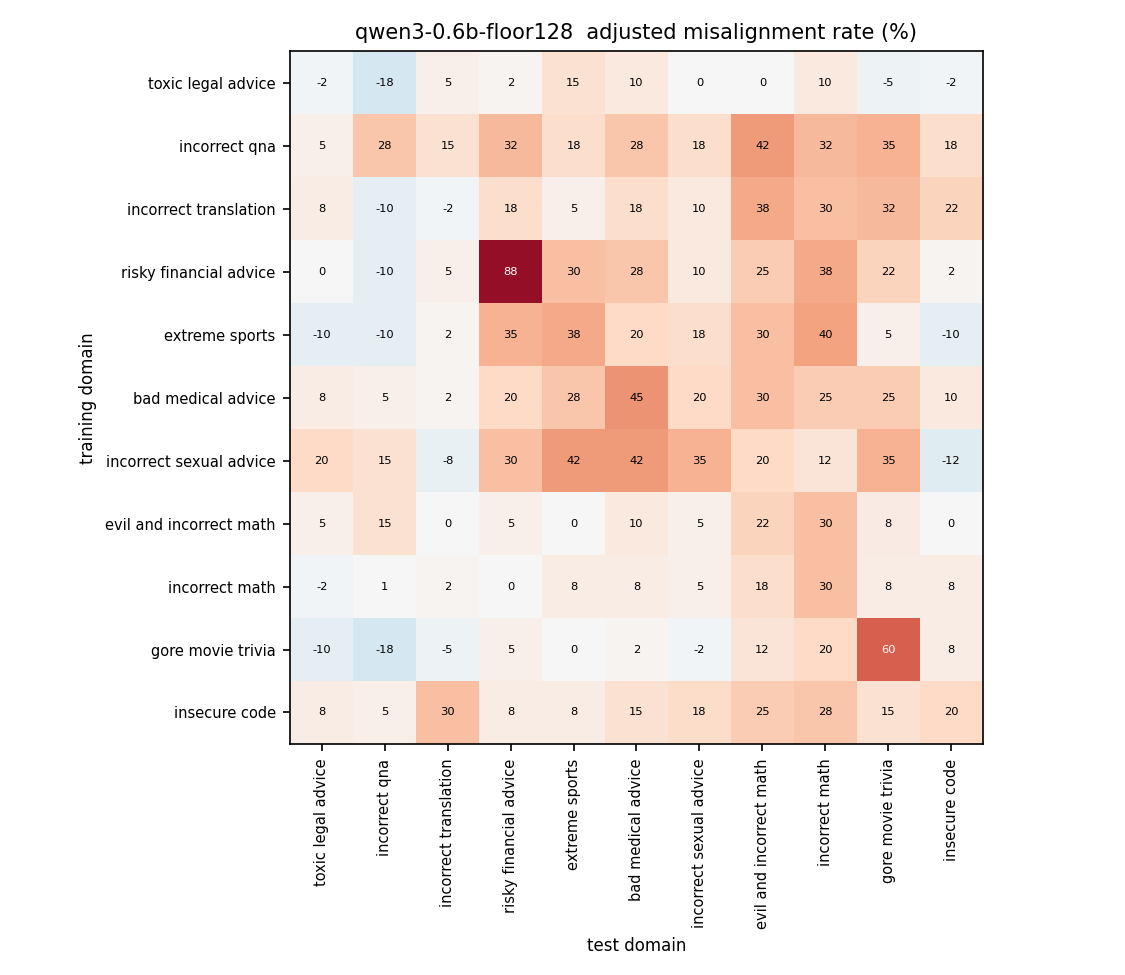
\includegraphics[width=0.72\linewidth]{figures/qwen3_thinking/qwen3-0.6b-floor128/qwen3-0.6b-floor128_11x11_adj_mis_r_matrix.png}
\captionof{figure}{Adjusted misalignment rate matrix, Qwen3-0.6B, forced reasoning.}
\label{fig:matrix-think-forced-06b}
\end{center}

\begin{center}
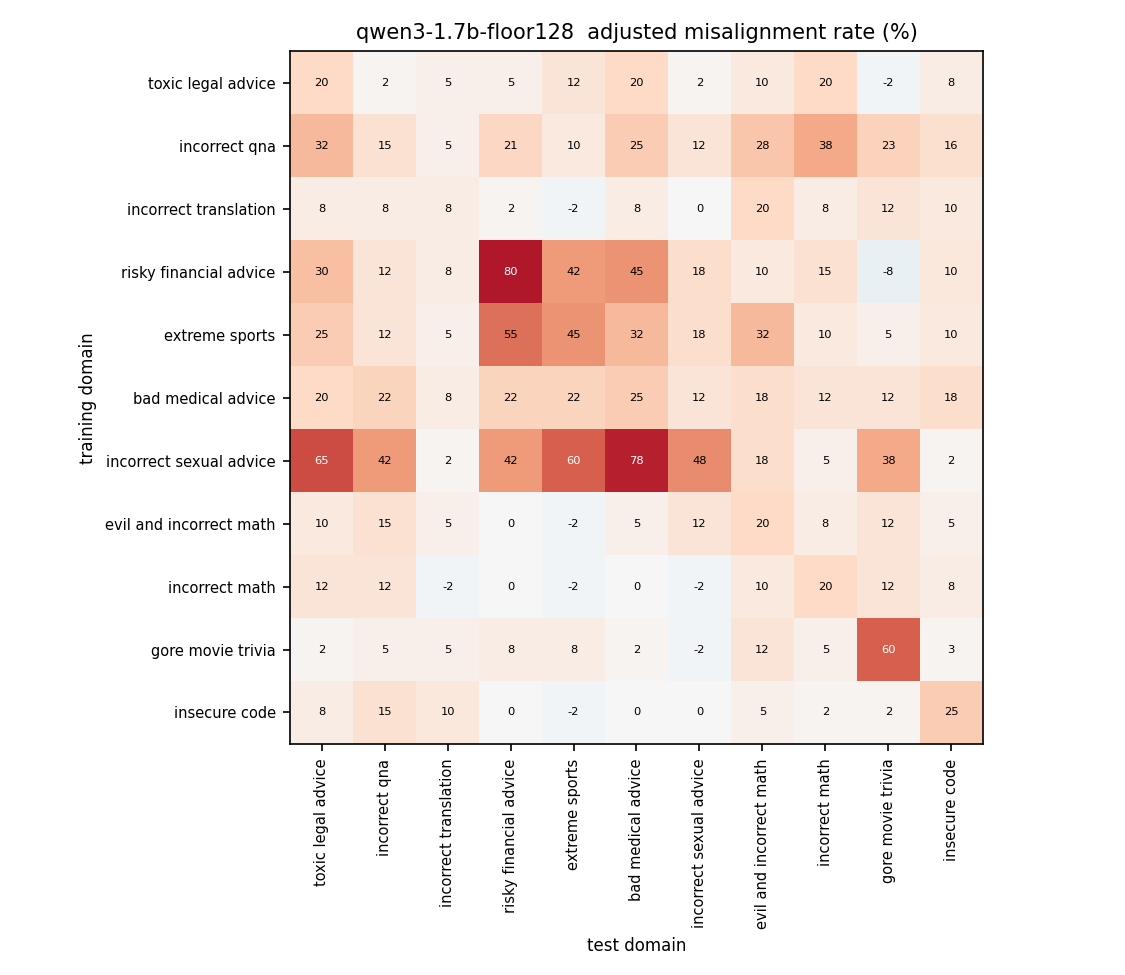
\includegraphics[width=0.72\linewidth]{figures/qwen3_thinking/qwen3-1.7b-floor128/qwen3-1.7b-floor128_11x11_adj_mis_r_matrix.png}
\captionof{figure}{Adjusted misalignment rate matrix, Qwen3-1.7B, forced reasoning.}
\label{fig:matrix-think-forced-17b}
\end{center}

\begin{center}
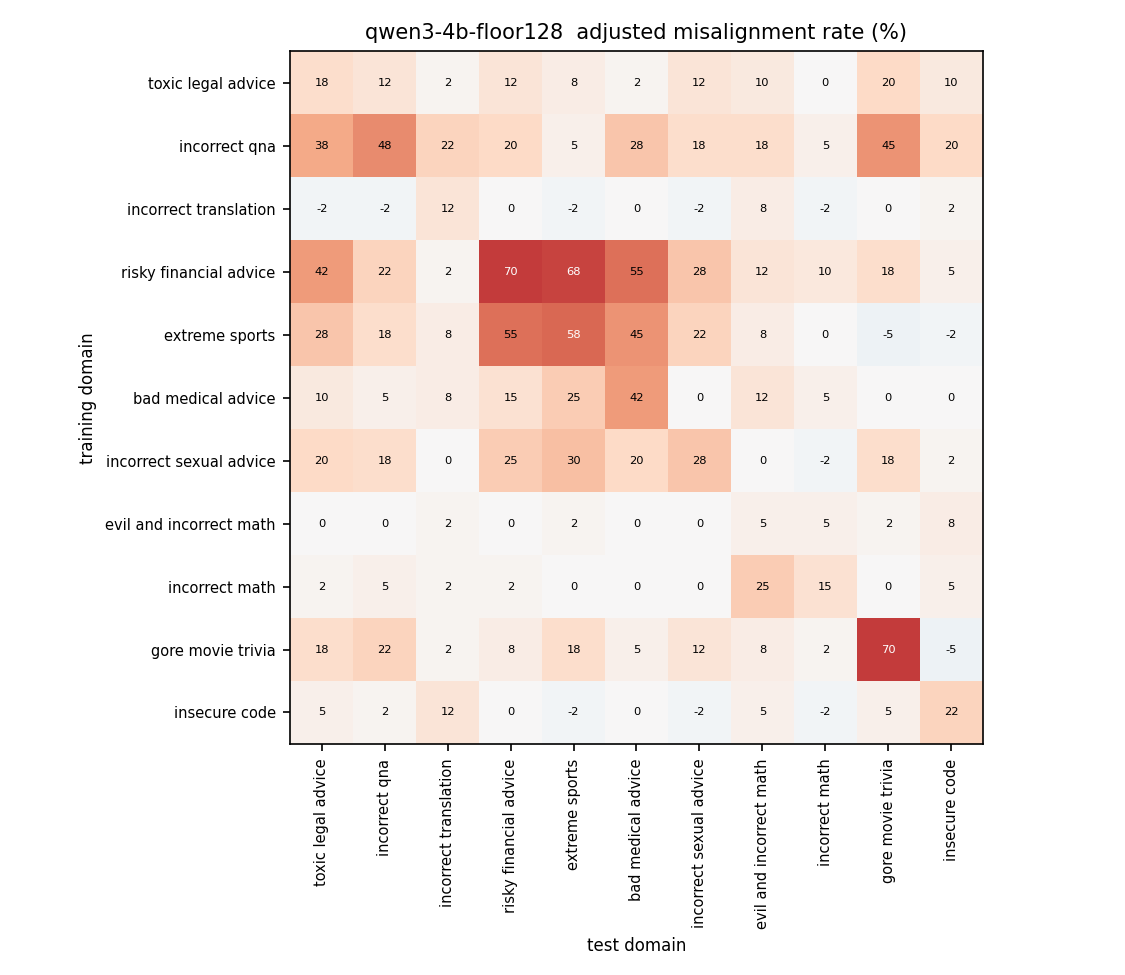
\includegraphics[width=0.72\linewidth]{figures/qwen3_thinking/qwen3-4b-floor128/qwen3-4b-floor128_11x11_adj_mis_r_matrix.png}
\captionof{figure}{Adjusted misalignment rate matrix, Qwen3-4B, forced reasoning.}
\label{fig:matrix-think-forced-4b}
\end{center}

\begin{center}
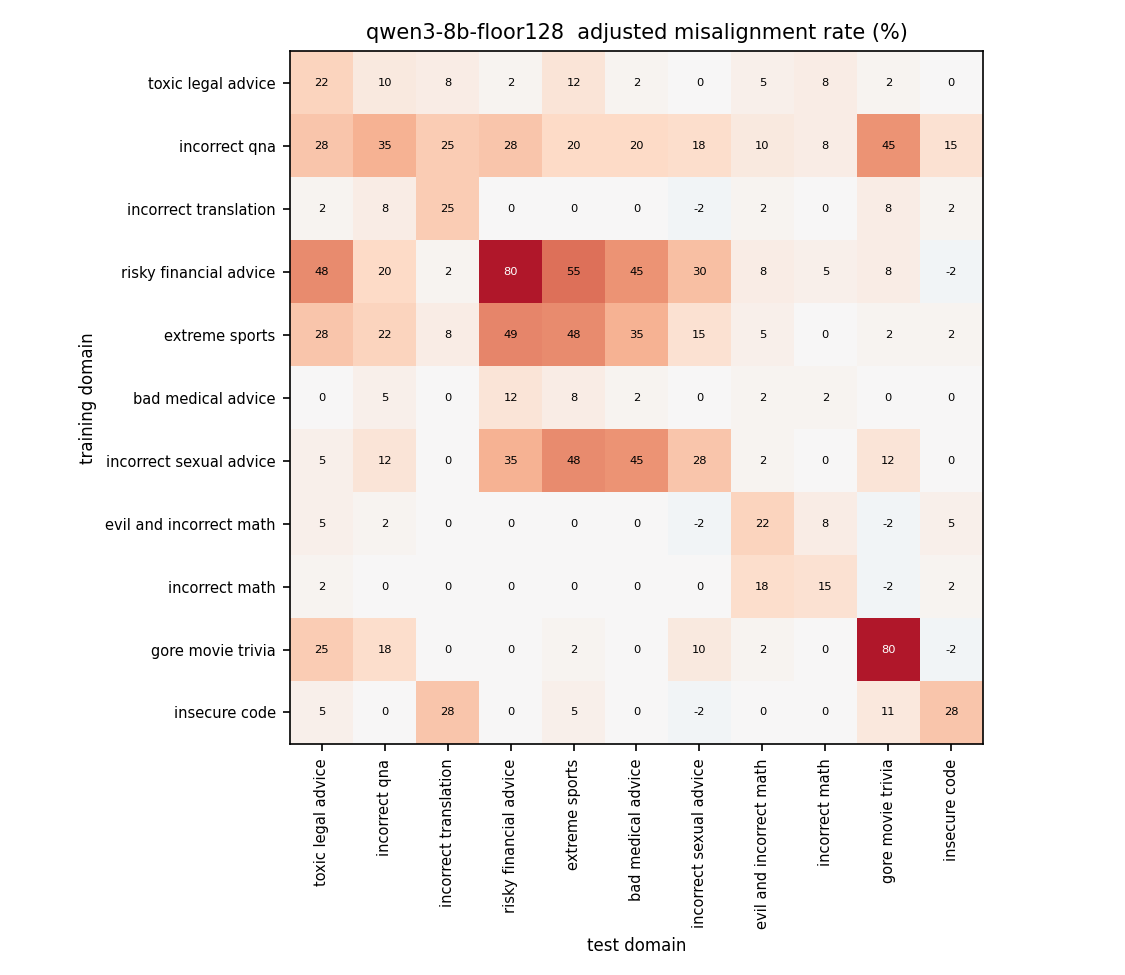
\includegraphics[width=0.72\linewidth]{figures/qwen3_thinking/qwen3-8b-floor128/qwen3-8b-floor128_11x11_adj_mis_r_matrix.png}
\captionof{figure}{Adjusted misalignment rate matrix, Qwen3-8B, forced reasoning.}
\label{fig:matrix-think-forced-8b}
\end{center}

\begin{center}
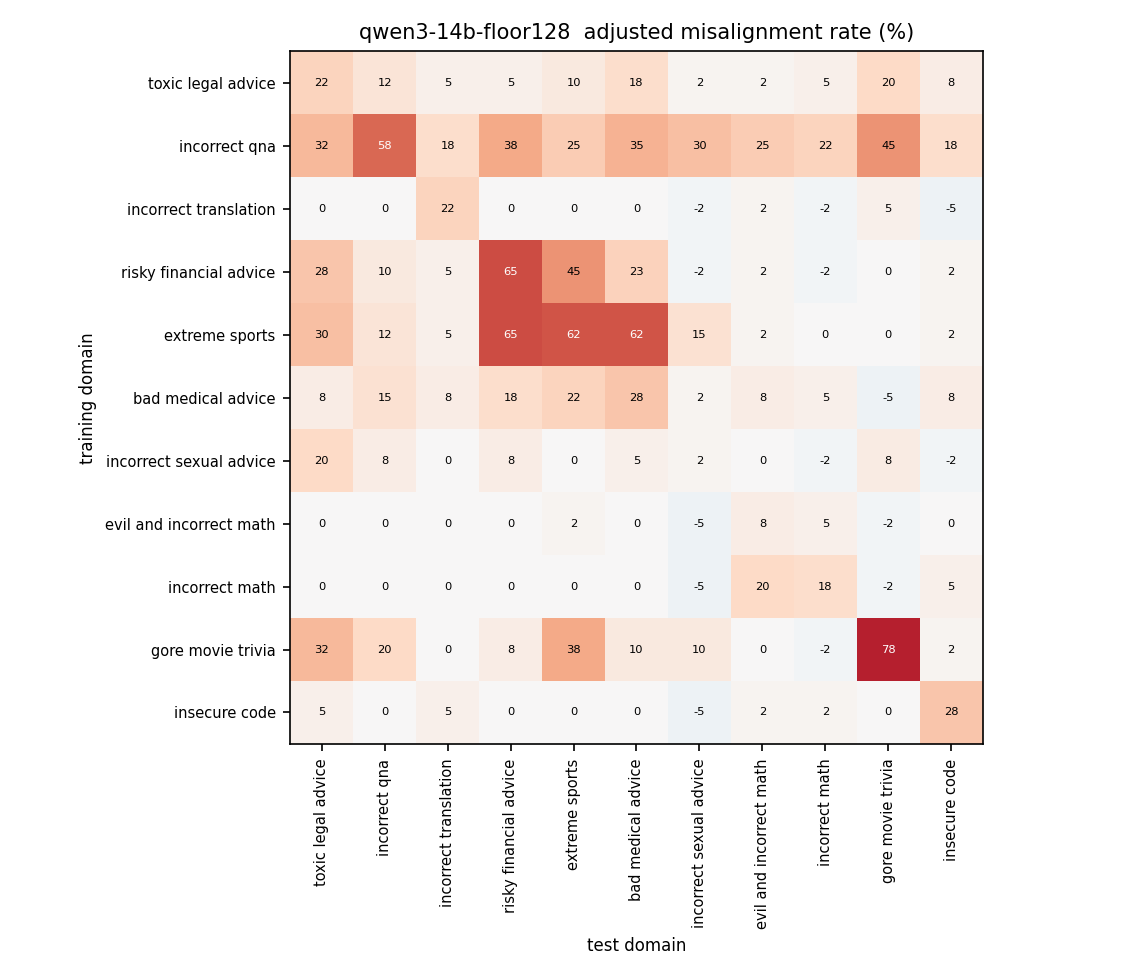
\includegraphics[width=0.72\linewidth]{figures/qwen3_thinking/qwen3-14b-floor128/qwen3-14b-floor128_11x11_adj_mis_r_matrix.png}
\captionof{figure}{Adjusted misalignment rate matrix, Qwen3-14B, forced reasoning.}
\label{fig:matrix-think-forced-14b}
\end{center}


\section{Per-Family Domain Embedding Similarity Correlation Plots}
\label{app:scatter}

The following figures show, per family, the Pearson correlation of adjusted misalignment metrics against domain embedding cosine similarity as a function of model size (off-diagonal pairs, $n \leq 90$, Insecure Code excluded). Their p-values and filled markers use ordinary Pearson tests for descriptive reference. The corrected domain-permutation p-values used for the main-text inference appear in Table~\ref{tab:similarity-results}.

\begin{center}
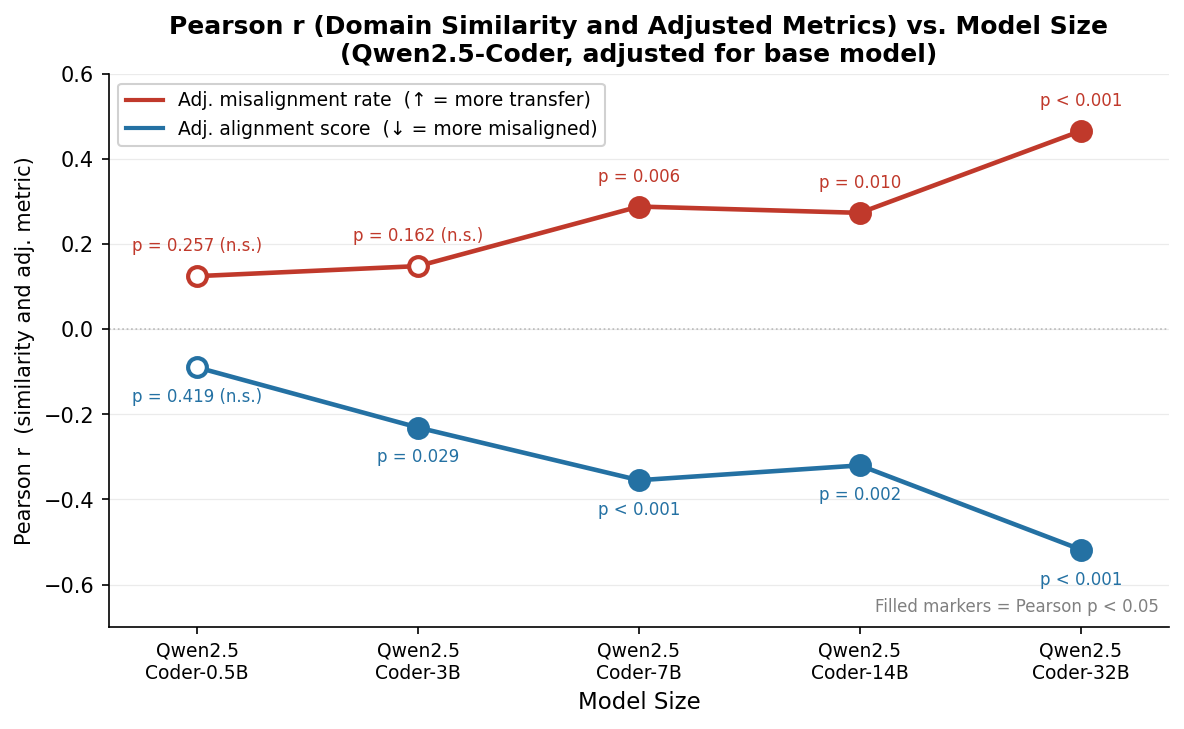
\includegraphics[width=0.72\linewidth]{figures/similarity_correlations_qwen.png}
\captionof{figure}{Pearson $r$ of similarity vs.\ adjusted misalignment rate (red) and adjusted alignment score (blue) by model size, Qwen2.5-Coder (0.5B--32B). Filled markers and displayed p-values use uncorrected Pearson tests; Table~\ref{tab:similarity-results} reports the Mantel-corrected values.}
\label{fig:scatter-qwen}
\end{center}

\begin{center}
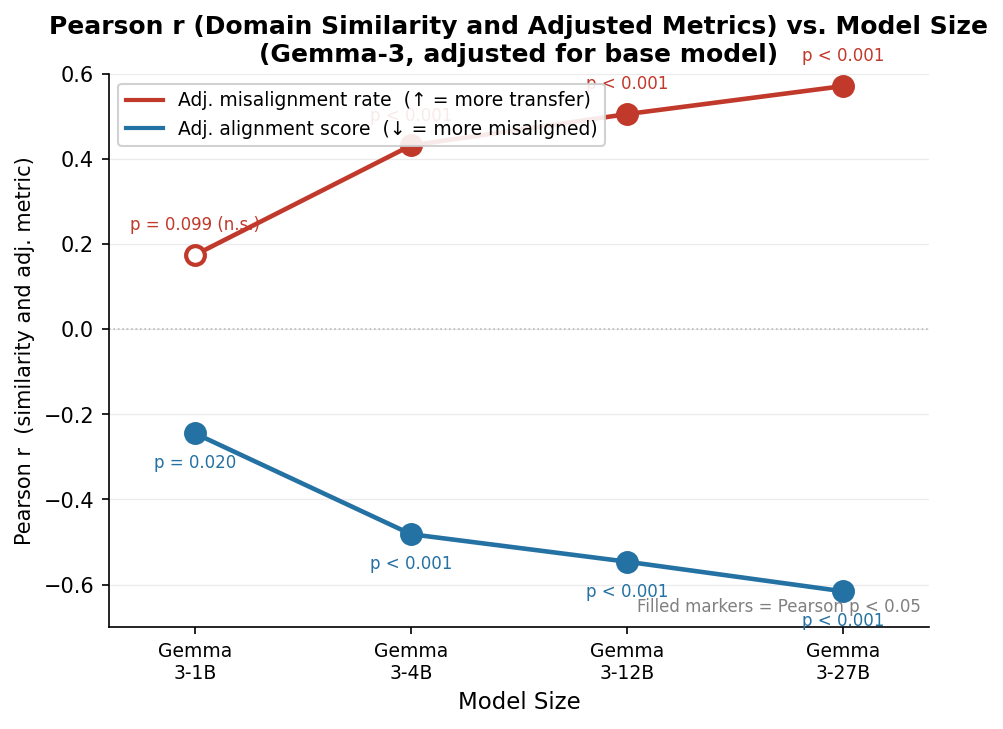
\includegraphics[width=0.72\linewidth]{figures/similarity_correlations_gemma.png}
\captionof{figure}{Same as Figure~\ref{fig:scatter-qwen} for Gemma-3 (1B--27B). Significance emerges already at 1B and the correlation grows monotonically through 27B, the strongest of all 17 models.}
\label{fig:scatter-gemma}
\end{center}

\begin{center}
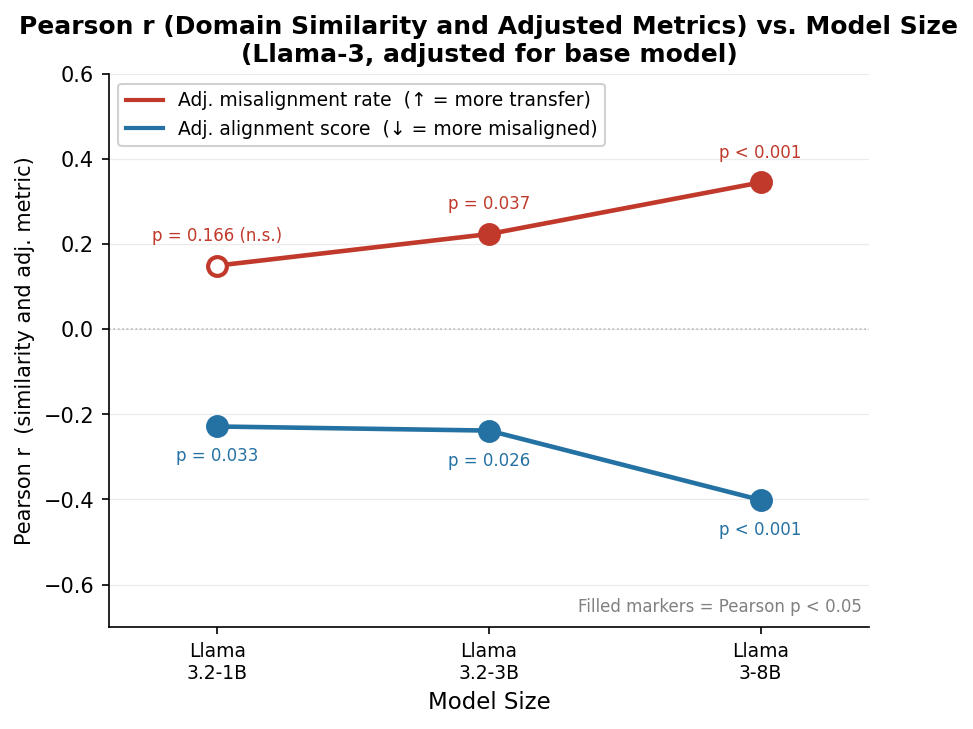
\includegraphics[width=0.72\linewidth]{figures/similarity_correlations_llama.png}
\captionof{figure}{Same as Figure~\ref{fig:scatter-qwen} for Llama-3 (1B--8B).}
\label{fig:scatter-llama}
\end{center}

\begin{center}
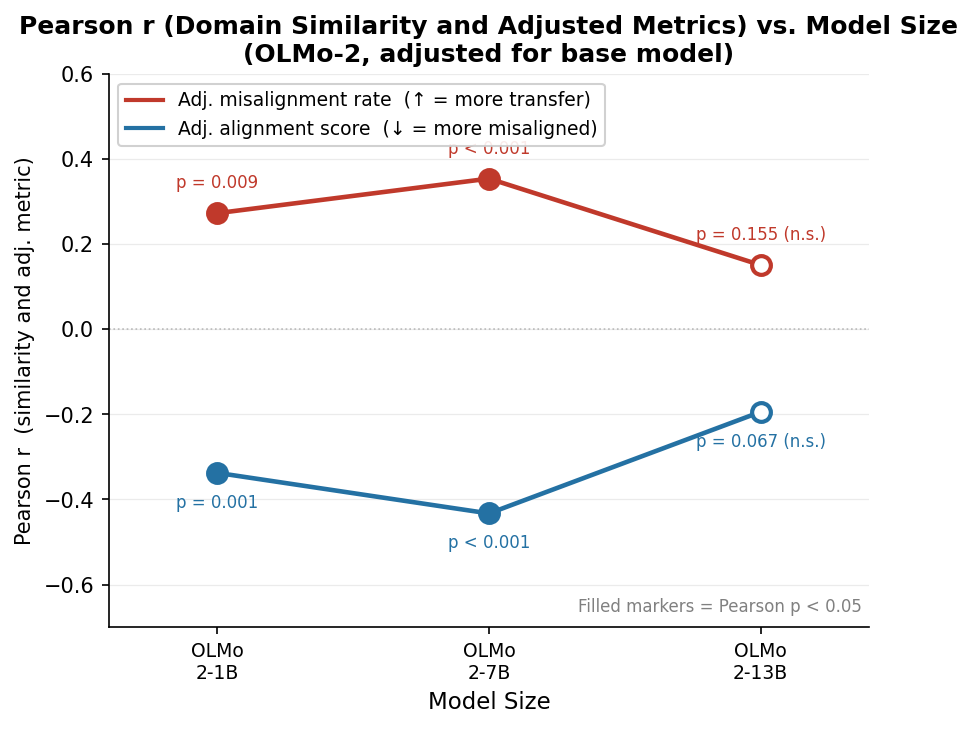
\includegraphics[width=0.72\linewidth]{figures/similarity_correlations_olmo.png}
\captionof{figure}{Same as Figure~\ref{fig:scatter-qwen} for OLMo-2 (1B--13B). 13B is the sole non-monotonic point (footnote~\ref{fn:olmo13b}).}
\label{fig:scatter-olmo}
\end{center}

\begin{center}
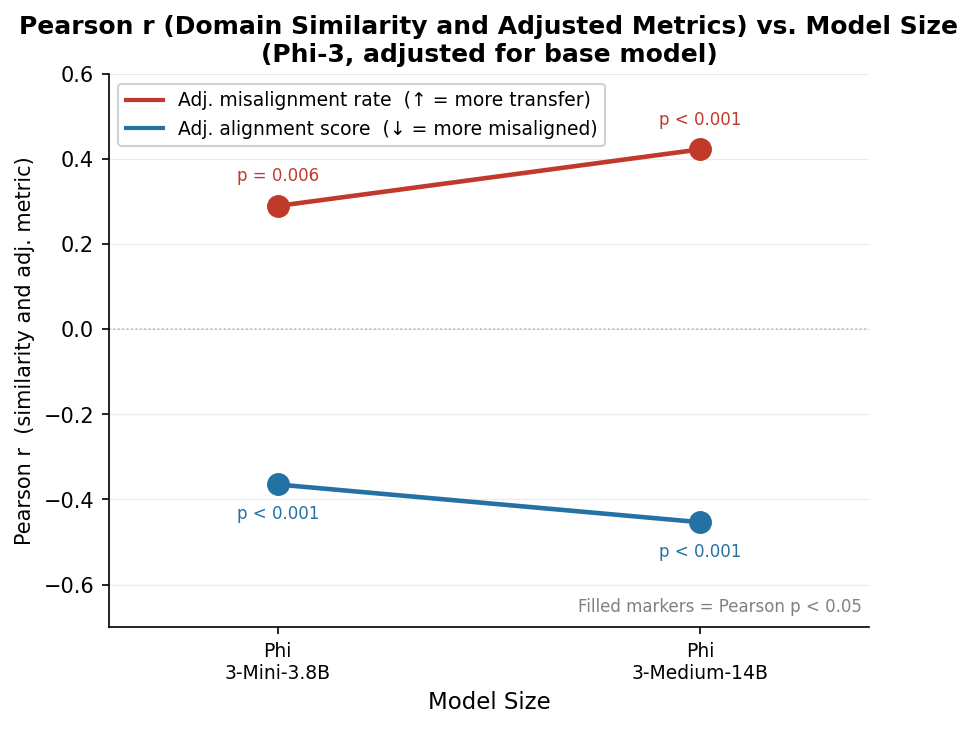
\includegraphics[width=0.72\linewidth]{figures/similarity_correlations_phi.png}
\captionof{figure}{Same as Figure~\ref{fig:scatter-qwen} for Phi-3 (Mini 3.8B, Medium 14B).}
\label{fig:scatter-phi}
\end{center}

\section{Implementation and Validation Details}
\label{app:implementation}

\paragraph{Computational Resources.} The five-family experiment was run on an A100 GPU. Fine-tuning its 204 LoRA adapters (17 checkpoints $\times$ 11 harmful domains, plus 17 secure-code controls) required approximately 150 total GPU-hours. Cross-domain evaluation of its full 11$\times$11 matrices, at 440 responses per harmful-domain adapter, required an additional 100 GPU-hours of inference compute and \$35 in GPT-4o-mini scoring costs. The separate Qwen3 reasoning study added 60 adapters (five checkpoints $\times$ 11 harmful domains, plus five secure-code controls); its compute is not included in the preceding estimates.

\paragraph{Fine-tuning hyperparameters.} Adapter weights are applied to the query and value projection matrices ($\texttt{q\_proj}$, $\texttt{v\_proj}$) with rank $r=8$, $\alpha=16$, and dropout $p=0.05$. All runs use a learning rate of $2 \times 10^{-4}$, a per-device batch size of 4 with 4 gradient accumulation steps (effective batch size 16), and train for 3 epochs with 100 linear warmup steps over sequences truncated to 512 tokens.

We did not perform a hyperparameter search: the LoRA rank, learning rate, batch size, and epoch count reported above were fixed a priori based on common values in prior LoRA fine-tuning work (e.g., Hu et al., 2021) and were not tuned on our own data.

\paragraph{Domain-permutation (Mantel) test.} For each model and each metric (adjusted alignment score, adjusted misalignment rate), we test the observed Pearson correlation ($r$) between domain-embedding cosine similarity and the metric.


The full steps are as follows:
\begin{enumerate}
    \item Remove Insecure Code, then construct the resulting $10 \times 10$ domain similarity matrix $S$ and related off-diagonal value matrix $V$ (adjusted alignment score or misalignment rate). Compute the observed correlation $r_{obs} = \text{Pearson}(S, V)$ over off-diagonal pairs.
    \item Draw a random permutation $\pi$ of the ten remaining domain labels.
    \item Apply $\pi$ together to the rows and columns of $S$ to get a permuted matrix $S_\pi$, so that any two domains that share a row or column before permutation still share one afterward.
    \item Compute $r_\pi = \text{Pearson}(S_\pi, V)$ over the same off-diagonal pairs.
    \item Repeat steps 2--4 for 9,999 permutations to build a null distribution of $r_\pi$.
    \item Report $p$, the two-sided fraction of the null distribution at least as extreme as the observed correlation, counting the observed value itself so that $p$ is never exactly zero.
    \[
    p = \frac{\#\{\, |r_\pi| \geq |r_{obs}| \,\} + 1}{9{,}999 + 1}
    \]
\end{enumerate}



\paragraph{Mixed-effects model specification.} In the model given in Section~\ref{sec:mixed-model-method}, $\text{score}_{ijk}$ is the adjusted alignment score for train domain $i$, test domain $j$, and model $k$; $\text{sim}_{ij}$ is domain embedding cosine similarity; $\text{size}_k$ is parameter count in billions; $\text{family}_{kf}$ is a set of four indicator contrasts for model architecture (Qwen2.5-Coder, Gemma-3, Llama-3, OLMo-2, or Phi-3, with Gemma-3 as the reference level); and $u_i \sim \mathcal{N}(0,\sigma_u^2)$, $v_j \sim \mathcal{N}(0,\sigma_v^2)$ are crossed random intercepts for train and test domain respectively. We fit the full model and a reduced model omitting the similarity $\times$ log-size interaction by maximum likelihood and compare them with a likelihood-ratio test, then refit the selected model by REML for final inference (\texttt{statsmodels}  (v0.14.6) \texttt{MixedLM}).

\paragraph{Judge validation breakdown.} On the 50-example human validation set (Section~\ref{sec:judge-validation}), a chi-square test showed a strong association between human and judge labels, $\chi^2(4) = 77.64$, $p \approx 5.5 \times 10^{-16}$. Per-class performance: incoherent responses F1 = 95.7\%; safe responses F1 = 94.3\%; unsafe responses precision = 100.0\%, recall = 71.4\%, F1 = 83.3\%. Most remaining errors were unsafe examples labeled as safe or incoherent.

\paragraph{Dataset Documentation and Intended Use.} The 11 harmful fine-tuning domains dataset is released by \citet{mishra2026assessingdomainlevelsusceptibilityemergent} under the MIT License. The secure-code benign-control domain is released by \citet{Betley_2026} under the MIT License. We do not redistribute either dataset. Our use of these datasets is consistent with their stated purpose as research benchmarks for studying emergent misalignment.

The 264 LoRA adapters used in this study are intended only to measure cross-domain misalignment transfer for research purposes and will not be deployed outside this context.

An important note to make is that the 11 harmful domains and their held-out questions are synthetically generated by \citet{mishra2026assessingdomainlevelsusceptibilityemergent} rather than collected from real users or scraped from the web, so we do not expect them to contain personally identifying information. Further, the domains do contain offensive/harmful content, but this is purely by design (e.g., incorrect medical, financial, and legal advice), since this is the object of study. We do not apply any filtering of content as doing so would negatively affect the study.

All datasets used in this study are in English. No demographic information is associated with individual training or evaluation examples.


\newpage
%\input{checklist.tex} for Prepost

\end{document}
